% Options for packages loaded elsewhere
\PassOptionsToPackage{unicode}{hyperref}
\PassOptionsToPackage{hyphens}{url}
%
\documentclass[
]{book}
\usepackage{amsmath,amssymb}
\usepackage{iftex}
\ifPDFTeX
  \usepackage[T1]{fontenc}
  \usepackage[utf8]{inputenc}
  \usepackage{textcomp} % provide euro and other symbols
\else % if luatex or xetex
  \usepackage{unicode-math} % this also loads fontspec
  \defaultfontfeatures{Scale=MatchLowercase}
  \defaultfontfeatures[\rmfamily]{Ligatures=TeX,Scale=1}
\fi
\usepackage{lmodern}
\ifPDFTeX\else
  % xetex/luatex font selection
\fi
% Use upquote if available, for straight quotes in verbatim environments
\IfFileExists{upquote.sty}{\usepackage{upquote}}{}
\IfFileExists{microtype.sty}{% use microtype if available
  \usepackage[]{microtype}
  \UseMicrotypeSet[protrusion]{basicmath} % disable protrusion for tt fonts
}{}
\makeatletter
\@ifundefined{KOMAClassName}{% if non-KOMA class
  \IfFileExists{parskip.sty}{%
    \usepackage{parskip}
  }{% else
    \setlength{\parindent}{0pt}
    \setlength{\parskip}{6pt plus 2pt minus 1pt}}
}{% if KOMA class
  \KOMAoptions{parskip=half}}
\makeatother
\usepackage{xcolor}
\usepackage{color}
\usepackage{fancyvrb}
\newcommand{\VerbBar}{|}
\newcommand{\VERB}{\Verb[commandchars=\\\{\}]}
\DefineVerbatimEnvironment{Highlighting}{Verbatim}{commandchars=\\\{\}}
% Add ',fontsize=\small' for more characters per line
\usepackage{framed}
\definecolor{shadecolor}{RGB}{248,248,248}
\newenvironment{Shaded}{\begin{snugshade}}{\end{snugshade}}
\newcommand{\AlertTok}[1]{\textcolor[rgb]{0.94,0.16,0.16}{#1}}
\newcommand{\AnnotationTok}[1]{\textcolor[rgb]{0.56,0.35,0.01}{\textbf{\textit{#1}}}}
\newcommand{\AttributeTok}[1]{\textcolor[rgb]{0.13,0.29,0.53}{#1}}
\newcommand{\BaseNTok}[1]{\textcolor[rgb]{0.00,0.00,0.81}{#1}}
\newcommand{\BuiltInTok}[1]{#1}
\newcommand{\CharTok}[1]{\textcolor[rgb]{0.31,0.60,0.02}{#1}}
\newcommand{\CommentTok}[1]{\textcolor[rgb]{0.56,0.35,0.01}{\textit{#1}}}
\newcommand{\CommentVarTok}[1]{\textcolor[rgb]{0.56,0.35,0.01}{\textbf{\textit{#1}}}}
\newcommand{\ConstantTok}[1]{\textcolor[rgb]{0.56,0.35,0.01}{#1}}
\newcommand{\ControlFlowTok}[1]{\textcolor[rgb]{0.13,0.29,0.53}{\textbf{#1}}}
\newcommand{\DataTypeTok}[1]{\textcolor[rgb]{0.13,0.29,0.53}{#1}}
\newcommand{\DecValTok}[1]{\textcolor[rgb]{0.00,0.00,0.81}{#1}}
\newcommand{\DocumentationTok}[1]{\textcolor[rgb]{0.56,0.35,0.01}{\textbf{\textit{#1}}}}
\newcommand{\ErrorTok}[1]{\textcolor[rgb]{0.64,0.00,0.00}{\textbf{#1}}}
\newcommand{\ExtensionTok}[1]{#1}
\newcommand{\FloatTok}[1]{\textcolor[rgb]{0.00,0.00,0.81}{#1}}
\newcommand{\FunctionTok}[1]{\textcolor[rgb]{0.13,0.29,0.53}{\textbf{#1}}}
\newcommand{\ImportTok}[1]{#1}
\newcommand{\InformationTok}[1]{\textcolor[rgb]{0.56,0.35,0.01}{\textbf{\textit{#1}}}}
\newcommand{\KeywordTok}[1]{\textcolor[rgb]{0.13,0.29,0.53}{\textbf{#1}}}
\newcommand{\NormalTok}[1]{#1}
\newcommand{\OperatorTok}[1]{\textcolor[rgb]{0.81,0.36,0.00}{\textbf{#1}}}
\newcommand{\OtherTok}[1]{\textcolor[rgb]{0.56,0.35,0.01}{#1}}
\newcommand{\PreprocessorTok}[1]{\textcolor[rgb]{0.56,0.35,0.01}{\textit{#1}}}
\newcommand{\RegionMarkerTok}[1]{#1}
\newcommand{\SpecialCharTok}[1]{\textcolor[rgb]{0.81,0.36,0.00}{\textbf{#1}}}
\newcommand{\SpecialStringTok}[1]{\textcolor[rgb]{0.31,0.60,0.02}{#1}}
\newcommand{\StringTok}[1]{\textcolor[rgb]{0.31,0.60,0.02}{#1}}
\newcommand{\VariableTok}[1]{\textcolor[rgb]{0.00,0.00,0.00}{#1}}
\newcommand{\VerbatimStringTok}[1]{\textcolor[rgb]{0.31,0.60,0.02}{#1}}
\newcommand{\WarningTok}[1]{\textcolor[rgb]{0.56,0.35,0.01}{\textbf{\textit{#1}}}}
\usepackage{longtable,booktabs,array}
\usepackage{calc} % for calculating minipage widths
% Correct order of tables after \paragraph or \subparagraph
\usepackage{etoolbox}
\makeatletter
\patchcmd\longtable{\par}{\if@noskipsec\mbox{}\fi\par}{}{}
\makeatother
% Allow footnotes in longtable head/foot
\IfFileExists{footnotehyper.sty}{\usepackage{footnotehyper}}{\usepackage{footnote}}
\makesavenoteenv{longtable}
\usepackage{graphicx}
\makeatletter
\def\maxwidth{\ifdim\Gin@nat@width>\linewidth\linewidth\else\Gin@nat@width\fi}
\def\maxheight{\ifdim\Gin@nat@height>\textheight\textheight\else\Gin@nat@height\fi}
\makeatother
% Scale images if necessary, so that they will not overflow the page
% margins by default, and it is still possible to overwrite the defaults
% using explicit options in \includegraphics[width, height, ...]{}
\setkeys{Gin}{width=\maxwidth,height=\maxheight,keepaspectratio}
% Set default figure placement to htbp
\makeatletter
\def\fps@figure{htbp}
\makeatother
\setlength{\emergencystretch}{3em} % prevent overfull lines
\providecommand{\tightlist}{%
  \setlength{\itemsep}{0pt}\setlength{\parskip}{0pt}}
\setcounter{secnumdepth}{5}
\usepackage{booktabs}
\ifLuaTeX
  \usepackage{selnolig}  % disable illegal ligatures
\fi
\usepackage[]{natbib}
\bibliographystyle{plainnat}
\IfFileExists{bookmark.sty}{\usepackage{bookmark}}{\usepackage{hyperref}}
\IfFileExists{xurl.sty}{\usepackage{xurl}}{} % add URL line breaks if available
\urlstyle{same}
\hypersetup{
  pdftitle={scRNAseq Analysis in R with Seurat},
  hidelinks,
  pdfcreator={LaTeX via pandoc}}

\title{scRNAseq Analysis in R with Seurat}
\author{}
\date{\vspace{-2.5em}2023-09-11}

\begin{document}
\maketitle

{
\setcounter{tocdepth}{1}
\tableofcontents
}
\hypertarget{about}{%
\chapter{About}\label{about}}

Material for scRNAseq analysis in R with Seurat workshop.

This workshop follows the introductory \href{https://satijalab.org/seurat/articles/pbmc3k_tutorial.html}{Guided Clustering Tutorial} tutorial from Seurat.

It is also drawing from a similar workshop held by Monash Bioinformatics Platform \href{https://monashbioinformaticsplatform.github.io/Single-Cell-Workshop/}{Single-Cell-Workshop}, with material \href{https://monashbioinformaticsplatform.github.io/Single-Cell-Workshop/pbmc3k_tutorial.html}{here}

\hypertarget{schedule}{%
\chapter{Schedule}\label{schedule}}

\hypertarget{day-2}{%
\subsection*{Day 2}\label{day-2}}
\addcontentsline{toc}{subsection}{Day 2}

\begin{longtable}[]{@{}ll@{}}
\toprule\noalign{}
Time & Content \\
\midrule\noalign{}
\endhead
\bottomrule\noalign{}
\endlastfoot
2:30 AEST & Session: Seurat Intro \\
3:30 AEST & Break \\
3:45 AEST & Session: QC \\
5:00 AEST & Finish \\
\end{longtable}

\hypertarget{day-2-1}{%
\subsection*{Day 2}\label{day-2-1}}
\addcontentsline{toc}{subsection}{Day 2}

\begin{longtable}[]{@{}ll@{}}
\toprule\noalign{}
Time & Content \\
\midrule\noalign{}
\endhead
\bottomrule\noalign{}
\endlastfoot
2:00 AEST & Session: Clustering and UMAP \\
3:30 AEST & Break \\
3:45 AEST & Session: Cell types and beyond \\
5:00 AEST & Finish \\
\end{longtable}

\hypertarget{part-content}{%
\part{Content}\label{part-content}}

\hypertarget{seuratobject}{%
\chapter{The Seurat object}\label{seuratobject}}

Most of todays workshop will be following the Seurat PBMC tutorial (reproduced in the next section).
We'll load raw counts data, do some QC and setup various useful information in a Seurat object.

But before that - what does a Seurat object look like, and what can we do with it once we've made one?

Lets have a look at a Seurat object that's already setup.

\hypertarget{load-an-existing-seurat-object}{%
\section{Load an existing Seurat object}\label{load-an-existing-seurat-object}}

The data we're working with today is a small dataset of about 3000 PBMCs (peripheral blood mononuclear cells) from a healthy donor. Just one sample.

This is an early demo dataset from 10X genomics (called pbmc3k) - you can find more information like qc reports \href{https://www.10xgenomics.com/resources/datasets/3-k-pbm-cs-from-a-healthy-donor-1-standard-1-1-0}{here}.

First, load Seurat package.

\begin{Shaded}
\begin{Highlighting}[]
\FunctionTok{library}\NormalTok{(Seurat)}
\end{Highlighting}
\end{Shaded}

And here's the one we prepared earlier. Seurat objects are usually saved as `.rds' files, which is an R format for storing binary data (not-text or human-readable). The functions \texttt{readRDS()} can load it.

\begin{Shaded}
\begin{Highlighting}[]
\NormalTok{pbmc\_processed }\OtherTok{\textless{}{-}} \FunctionTok{readRDS}\NormalTok{(}\StringTok{"data/pbmc\_tutorial.rds"}\NormalTok{)}
\NormalTok{pbmc\_processed}
\CommentTok{\#\textgreater{} An object of class Seurat }
\CommentTok{\#\textgreater{} 13714 features across 2700 samples within 1 assay }
\CommentTok{\#\textgreater{} Active assay: RNA (13714 features, 2000 variable features)}
\CommentTok{\#\textgreater{}  2 dimensional reductions calculated: pca, umap}
\end{Highlighting}
\end{Shaded}

\hypertarget{whats-in-there}{%
\section{What's in there?}\label{whats-in-there}}

Some of the most important information for working with Seurat objects is in the metadata.
This is cell level information - each row is one cell, identified by its barcode.
Extra information gets added to this table as analysis progresses.

\begin{Shaded}
\begin{Highlighting}[]
\FunctionTok{head}\NormalTok{(pbmc\_processed}\SpecialCharTok{@}\NormalTok{meta.data)}
\CommentTok{\#\textgreater{}                  orig.ident nCount\_RNA nFeature\_RNA}
\CommentTok{\#\textgreater{} AAACATACAACCAC{-}1     pbmc3k       2419          779}
\CommentTok{\#\textgreater{} AAACATTGAGCTAC{-}1     pbmc3k       4903         1352}
\CommentTok{\#\textgreater{} AAACATTGATCAGC{-}1     pbmc3k       3147         1129}
\CommentTok{\#\textgreater{} AAACCGTGCTTCCG{-}1     pbmc3k       2639          960}
\CommentTok{\#\textgreater{} AAACCGTGTATGCG{-}1     pbmc3k        980          521}
\CommentTok{\#\textgreater{} AAACGCACTGGTAC{-}1     pbmc3k       2163          781}
\CommentTok{\#\textgreater{}                  percent.mt RNA\_snn\_res.0.5 seurat\_clusters}
\CommentTok{\#\textgreater{} AAACATACAACCAC{-}1  3.0177759               0               0}
\CommentTok{\#\textgreater{} AAACATTGAGCTAC{-}1  3.7935958               3               3}
\CommentTok{\#\textgreater{} AAACATTGATCAGC{-}1  0.8897363               2               2}
\CommentTok{\#\textgreater{} AAACCGTGCTTCCG{-}1  1.7430845               5               5}
\CommentTok{\#\textgreater{} AAACCGTGTATGCG{-}1  1.2244898               6               6}
\CommentTok{\#\textgreater{} AAACGCACTGGTAC{-}1  1.6643551               2               2}
\end{Highlighting}
\end{Shaded}

That doesn't have any gene expression though, that's stored in an `Assay'.
The Assay structure has some nuances (see discussion below), but there are functions that get the assay data out for you.

By default this object will return the normalised data (from the only assay in this object, called RNA). Every `.' is a zero.

\begin{Shaded}
\begin{Highlighting}[]
\FunctionTok{GetAssayData}\NormalTok{(pbmc\_processed)[}\DecValTok{1}\SpecialCharTok{:}\DecValTok{15}\NormalTok{,}\DecValTok{1}\SpecialCharTok{:}\DecValTok{5}\NormalTok{]}
\CommentTok{\#\textgreater{} 15 x 5 sparse Matrix of class "dgCMatrix"}
\CommentTok{\#\textgreater{}               AAACATACAACCAC{-}1 AAACATTGAGCTAC{-}1}
\CommentTok{\#\textgreater{} AL627309.1                   .         .       }
\CommentTok{\#\textgreater{} AP006222.2                   .         .       }
\CommentTok{\#\textgreater{} RP11{-}206L10.2                .         .       }
\CommentTok{\#\textgreater{} RP11{-}206L10.9                .         .       }
\CommentTok{\#\textgreater{} LINC00115                    .         .       }
\CommentTok{\#\textgreater{} NOC2L                        .         .       }
\CommentTok{\#\textgreater{} KLHL17                       .         .       }
\CommentTok{\#\textgreater{} PLEKHN1                      .         .       }
\CommentTok{\#\textgreater{} RP11{-}54O7.17                 .         .       }
\CommentTok{\#\textgreater{} HES4                         .         .       }
\CommentTok{\#\textgreater{} RP11{-}54O7.11                 .         .       }
\CommentTok{\#\textgreater{} ISG15                        .         .       }
\CommentTok{\#\textgreater{} AGRN                         .         .       }
\CommentTok{\#\textgreater{} C1orf159                     .         .       }
\CommentTok{\#\textgreater{} TNFRSF18                     .         1.625141}
\CommentTok{\#\textgreater{}               AAACATTGATCAGC{-}1 AAACCGTGCTTCCG{-}1}
\CommentTok{\#\textgreater{} AL627309.1            .                 .      }
\CommentTok{\#\textgreater{} AP006222.2            .                 .      }
\CommentTok{\#\textgreater{} RP11{-}206L10.2         .                 .      }
\CommentTok{\#\textgreater{} RP11{-}206L10.9         .                 .      }
\CommentTok{\#\textgreater{} LINC00115             .                 .      }
\CommentTok{\#\textgreater{} NOC2L                 .                 .      }
\CommentTok{\#\textgreater{} KLHL17                .                 .      }
\CommentTok{\#\textgreater{} PLEKHN1               .                 .      }
\CommentTok{\#\textgreater{} RP11{-}54O7.17          .                 .      }
\CommentTok{\#\textgreater{} HES4                  .                 .      }
\CommentTok{\#\textgreater{} RP11{-}54O7.11          .                 .      }
\CommentTok{\#\textgreater{} ISG15                 1.429744          3.55831}
\CommentTok{\#\textgreater{} AGRN                  .                 .      }
\CommentTok{\#\textgreater{} C1orf159              .                 .      }
\CommentTok{\#\textgreater{} TNFRSF18              .                 .      }
\CommentTok{\#\textgreater{}               AAACCGTGTATGCG{-}1}
\CommentTok{\#\textgreater{} AL627309.1                   .}
\CommentTok{\#\textgreater{} AP006222.2                   .}
\CommentTok{\#\textgreater{} RP11{-}206L10.2                .}
\CommentTok{\#\textgreater{} RP11{-}206L10.9                .}
\CommentTok{\#\textgreater{} LINC00115                    .}
\CommentTok{\#\textgreater{} NOC2L                        .}
\CommentTok{\#\textgreater{} KLHL17                       .}
\CommentTok{\#\textgreater{} PLEKHN1                      .}
\CommentTok{\#\textgreater{} RP11{-}54O7.17                 .}
\CommentTok{\#\textgreater{} HES4                         .}
\CommentTok{\#\textgreater{} RP11{-}54O7.11                 .}
\CommentTok{\#\textgreater{} ISG15                        .}
\CommentTok{\#\textgreater{} AGRN                         .}
\CommentTok{\#\textgreater{} C1orf159                     .}
\CommentTok{\#\textgreater{} TNFRSF18                     .}
\end{Highlighting}
\end{Shaded}

But the raw counts data is accessible too.

\begin{Shaded}
\begin{Highlighting}[]
\FunctionTok{GetAssayData}\NormalTok{(pbmc\_processed, }\AttributeTok{slot=}\StringTok{\textquotesingle{}counts\textquotesingle{}}\NormalTok{)[}\DecValTok{1}\SpecialCharTok{:}\DecValTok{15}\NormalTok{,}\DecValTok{1}\SpecialCharTok{:}\DecValTok{5}\NormalTok{]}
\CommentTok{\#\textgreater{} 15 x 5 sparse Matrix of class "dgCMatrix"}
\CommentTok{\#\textgreater{}               AAACATACAACCAC{-}1 AAACATTGAGCTAC{-}1}
\CommentTok{\#\textgreater{} AL627309.1                   .                .}
\CommentTok{\#\textgreater{} AP006222.2                   .                .}
\CommentTok{\#\textgreater{} RP11{-}206L10.2                .                .}
\CommentTok{\#\textgreater{} RP11{-}206L10.9                .                .}
\CommentTok{\#\textgreater{} LINC00115                    .                .}
\CommentTok{\#\textgreater{} NOC2L                        .                .}
\CommentTok{\#\textgreater{} KLHL17                       .                .}
\CommentTok{\#\textgreater{} PLEKHN1                      .                .}
\CommentTok{\#\textgreater{} RP11{-}54O7.17                 .                .}
\CommentTok{\#\textgreater{} HES4                         .                .}
\CommentTok{\#\textgreater{} RP11{-}54O7.11                 .                .}
\CommentTok{\#\textgreater{} ISG15                        .                .}
\CommentTok{\#\textgreater{} AGRN                         .                .}
\CommentTok{\#\textgreater{} C1orf159                     .                .}
\CommentTok{\#\textgreater{} TNFRSF18                     .                2}
\CommentTok{\#\textgreater{}               AAACATTGATCAGC{-}1 AAACCGTGCTTCCG{-}1}
\CommentTok{\#\textgreater{} AL627309.1                   .                .}
\CommentTok{\#\textgreater{} AP006222.2                   .                .}
\CommentTok{\#\textgreater{} RP11{-}206L10.2                .                .}
\CommentTok{\#\textgreater{} RP11{-}206L10.9                .                .}
\CommentTok{\#\textgreater{} LINC00115                    .                .}
\CommentTok{\#\textgreater{} NOC2L                        .                .}
\CommentTok{\#\textgreater{} KLHL17                       .                .}
\CommentTok{\#\textgreater{} PLEKHN1                      .                .}
\CommentTok{\#\textgreater{} RP11{-}54O7.17                 .                .}
\CommentTok{\#\textgreater{} HES4                         .                .}
\CommentTok{\#\textgreater{} RP11{-}54O7.11                 .                .}
\CommentTok{\#\textgreater{} ISG15                        1                9}
\CommentTok{\#\textgreater{} AGRN                         .                .}
\CommentTok{\#\textgreater{} C1orf159                     .                .}
\CommentTok{\#\textgreater{} TNFRSF18                     .                .}
\CommentTok{\#\textgreater{}               AAACCGTGTATGCG{-}1}
\CommentTok{\#\textgreater{} AL627309.1                   .}
\CommentTok{\#\textgreater{} AP006222.2                   .}
\CommentTok{\#\textgreater{} RP11{-}206L10.2                .}
\CommentTok{\#\textgreater{} RP11{-}206L10.9                .}
\CommentTok{\#\textgreater{} LINC00115                    .}
\CommentTok{\#\textgreater{} NOC2L                        .}
\CommentTok{\#\textgreater{} KLHL17                       .}
\CommentTok{\#\textgreater{} PLEKHN1                      .}
\CommentTok{\#\textgreater{} RP11{-}54O7.17                 .}
\CommentTok{\#\textgreater{} HES4                         .}
\CommentTok{\#\textgreater{} RP11{-}54O7.11                 .}
\CommentTok{\#\textgreater{} ISG15                        .}
\CommentTok{\#\textgreater{} AGRN                         .}
\CommentTok{\#\textgreater{} C1orf159                     .}
\CommentTok{\#\textgreater{} TNFRSF18                     .}
\end{Highlighting}
\end{Shaded}

Seurat generally hides alot of this data complexity, and provides functions for typical tasks. Like plotting.

\hypertarget{plotting}{%
\section{Plotting}\label{plotting}}

Lets plot a classic UMAP with \texttt{DimPlot}- defaults to the clusters on a `umap' view.

\begin{Shaded}
\begin{Highlighting}[]
\FunctionTok{DimPlot}\NormalTok{(pbmc\_processed)}
\end{Highlighting}
\end{Shaded}

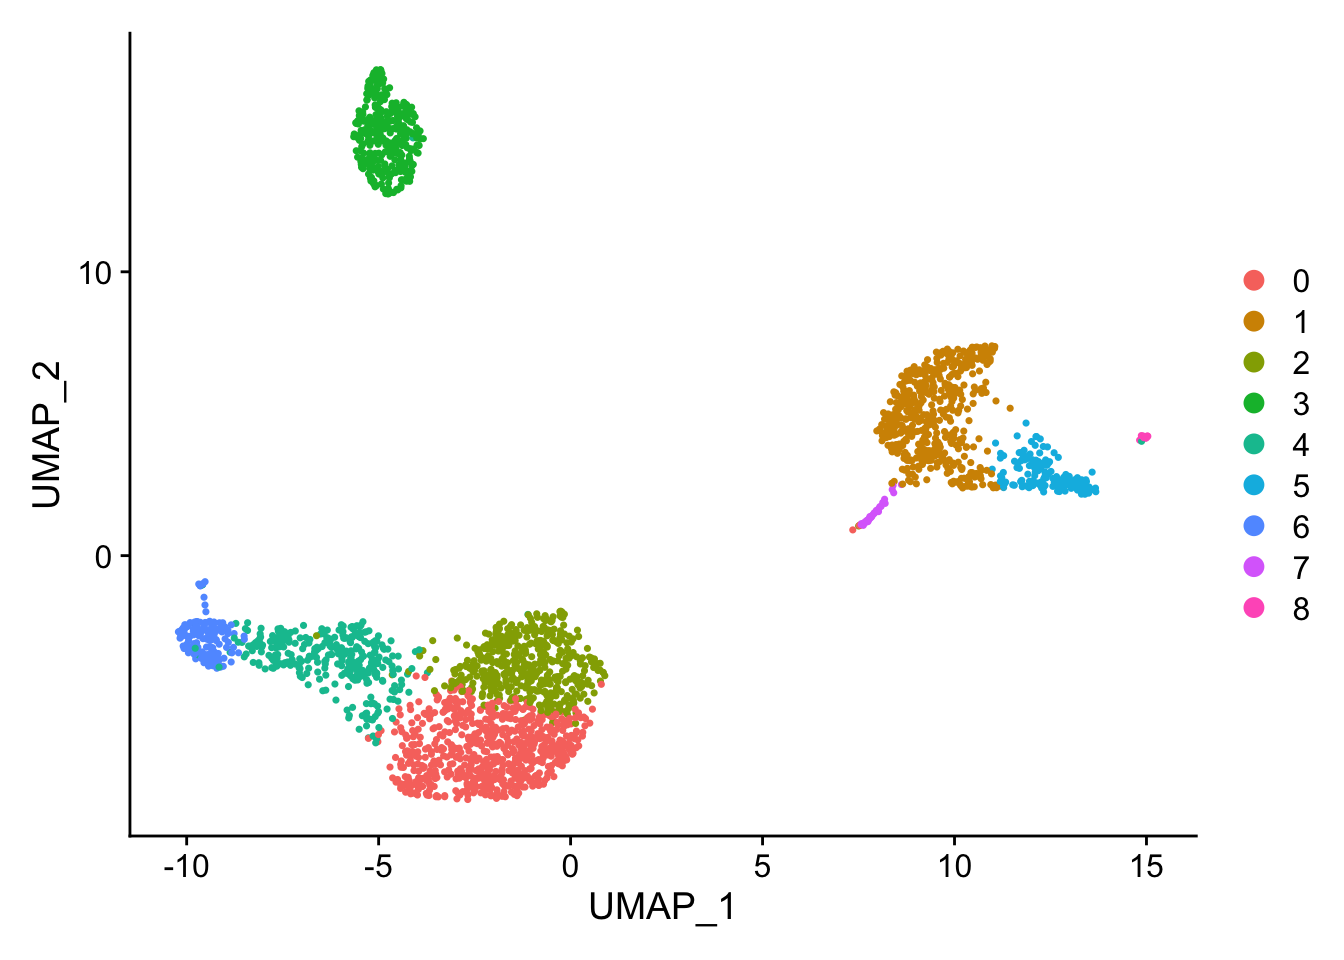
\includegraphics{scRNAseqInR_Doco_files/figure-latex/unnamed-chunk-9-1.pdf}

\begin{Shaded}
\begin{Highlighting}[]
\CommentTok{\# equivalent to}
\CommentTok{\#DimPlot(pbmc\_processed, reduction = \textquotesingle{}umap\textquotesingle{})}
\end{Highlighting}
\end{Shaded}

What about checking some gene expression? Genes are called `features' in a Seurat object (because if it was CITE-seq they'd be proteins!). So the \texttt{FeaturePlot()} function will show gene expression.

\begin{Shaded}
\begin{Highlighting}[]
\FunctionTok{FeaturePlot}\NormalTok{(pbmc\_processed, }\AttributeTok{features =}  \StringTok{"CD14"}\NormalTok{)}
\end{Highlighting}
\end{Shaded}

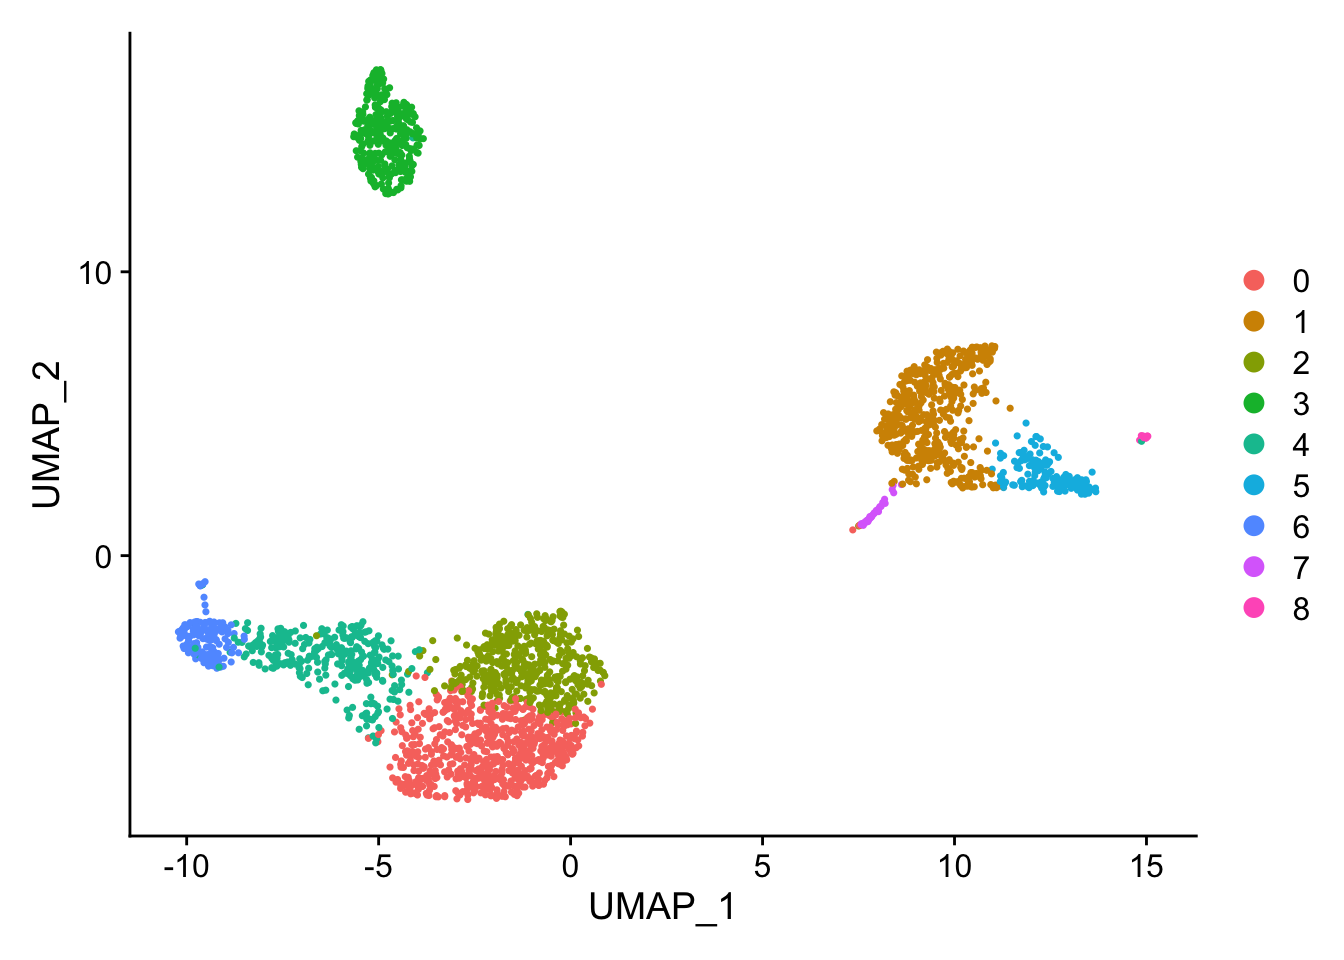
\includegraphics{scRNAseqInR_Doco_files/figure-latex/unnamed-chunk-10-1.pdf}

It also works for continuous cell-level data - any column in the metadata table.

\begin{Shaded}
\begin{Highlighting}[]
\FunctionTok{FeaturePlot}\NormalTok{(pbmc\_processed, }\AttributeTok{features =}  \StringTok{"percent.mt"}\NormalTok{)}
\end{Highlighting}
\end{Shaded}

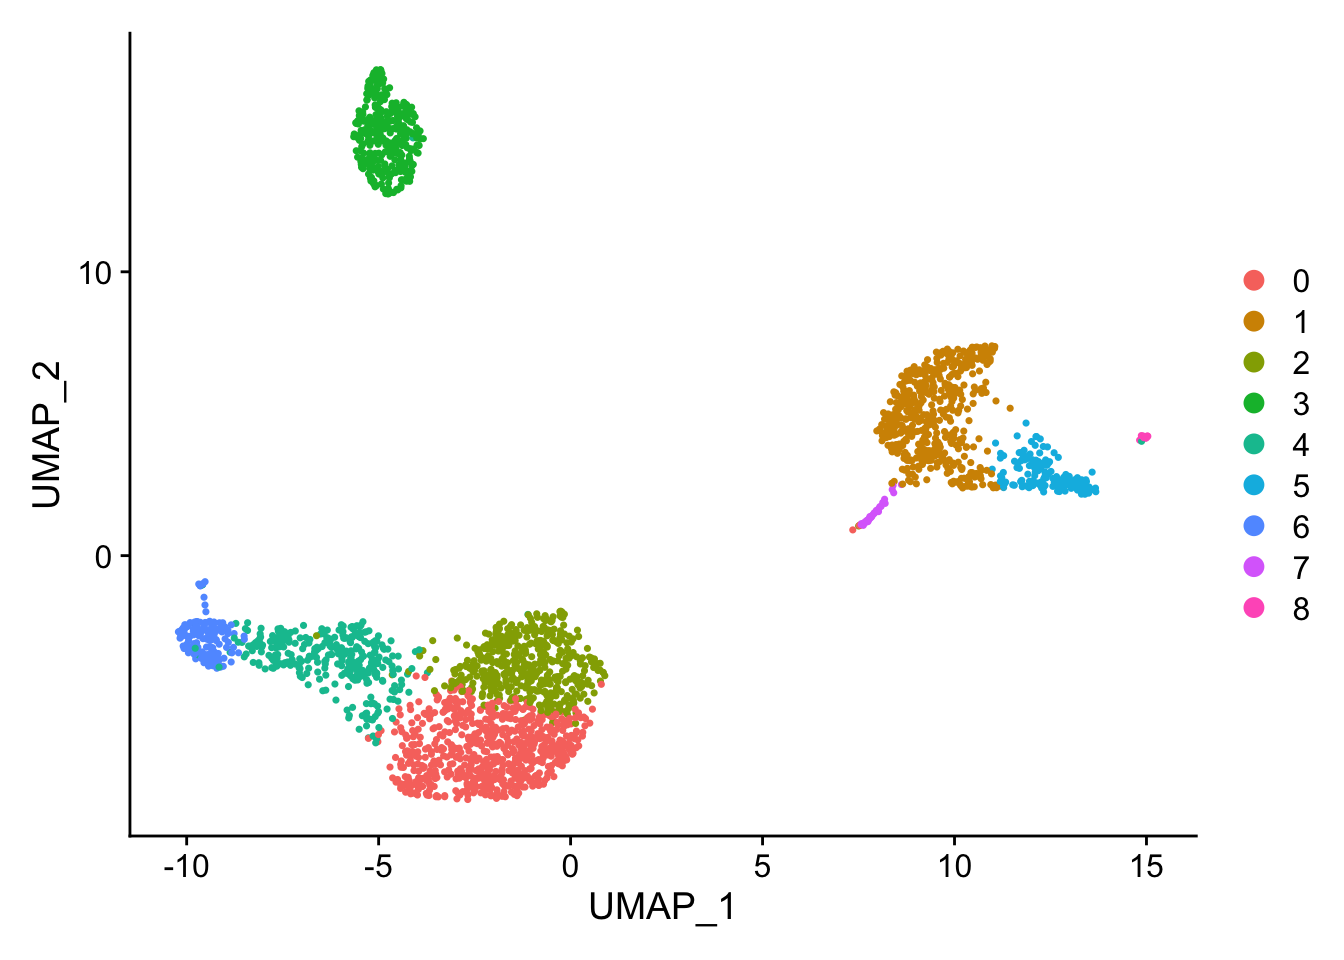
\includegraphics{scRNAseqInR_Doco_files/figure-latex/unnamed-chunk-11-1.pdf}

And what about showing CD14 expression across which clusters (or any other categorical information in the metadata)

\begin{Shaded}
\begin{Highlighting}[]
\FunctionTok{VlnPlot}\NormalTok{(pbmc\_processed, }\AttributeTok{features =} \StringTok{\textquotesingle{}CD14\textquotesingle{}}\NormalTok{)}
\end{Highlighting}
\end{Shaded}

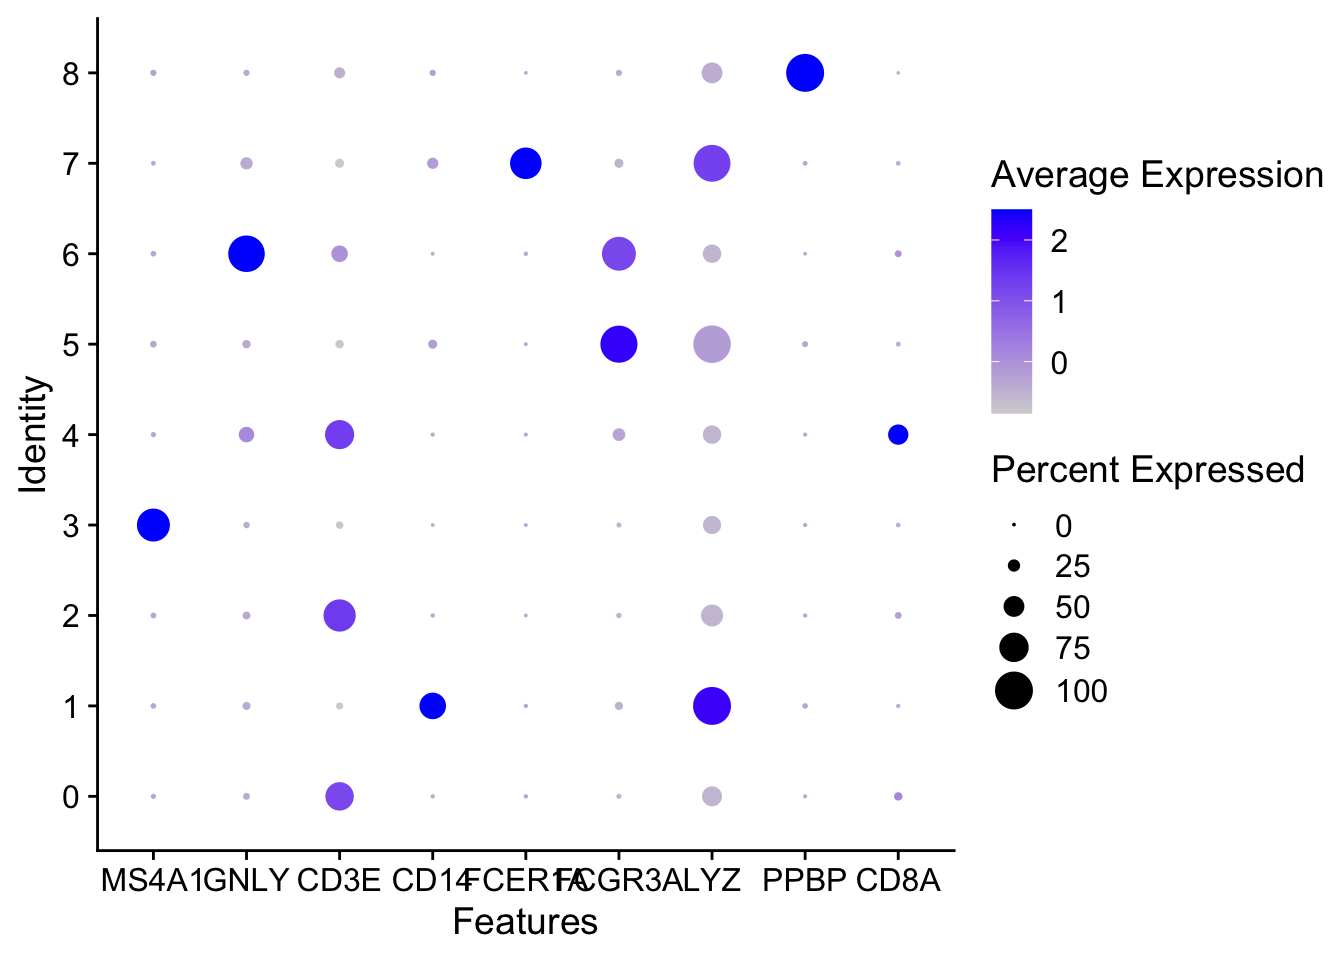
\includegraphics{scRNAseqInR_Doco_files/figure-latex/unnamed-chunk-12-1.pdf}

\hypertarget{challenge-plotting}{%
\subsubsection*{Challenge: Plotting}\label{challenge-plotting}}
\addcontentsline{toc}{subsubsection}{Challenge: Plotting}

Plot your favourite gene. What cluster is it found in?

Tip: You can check if the gene is in the dataset by looking for it in the rownames of the seurat object \texttt{"CCT3"\ \%in\%\ rownames(pbmc\_processed)}

\begin{center}\rule{0.5\linewidth}{0.5pt}\end{center}

\hypertarget{discussion-the-seurat-object-in-r}{%
\subsubsection*{Discussion: The Seurat Object in R}\label{discussion-the-seurat-object-in-r}}
\addcontentsline{toc}{subsubsection}{Discussion: The Seurat Object in R}

Lets take a look at the seurat object we have just created in R, \texttt{pbmc\_processed}

To accomodate the complexity of data arising from a single cell RNA seq experiment, the seurat object keeps this as a container of multiple data tables that are linked.

The functions in seurat can access parts of the data object for analysis and visualisation, we will cover this later on.

There are a couple of concepts to discuss here.

\textbf{Class}

These are essentially data containers in R as a class, and can accessed as a variable in the R environment.

Classes are pre-defined and can contain multiple data tables and metadata. For Seurat, there are three types.

\begin{itemize}
\tightlist
\item
  Seurat - the main data class, contains all the data.
\item
  Assay - found within the Seurat object. Depending on the experiment a cell could have data on RNA, ATAC etc measured
\item
  DimReduc - for PCA and UMAP
\end{itemize}

\textbf{Slots}

Slots are parts within a class that contain specific data. These can be lists, data tables and vectors and can be accessed with conventional R methods.

\textbf{Data Access}

Many of the functions in Seurat operate on the data class and slots within them seamlessly. There maybe occasion to access these separately to \texttt{hack} them, however this is an advanced analysis method.

The ways to access the slots can be through methods for the class (functions) or with standard R accessor nomenclature.

\textbf{Examples of accessing a Seurat object}

The \texttt{assays} slot in \texttt{pbmc\_processed} can be accessed with \texttt{pbmc\_processed@assays}.

The \texttt{RNA} assay can be accessed from this with \texttt{pbmc\_processed@assays\$RNA}.

We often want to access assays, so Seurat nicely gives us a shortcut \texttt{pbmc\_processed\$RNA}. You may sometimes see an alternative notation \texttt{pbmc\_processed{[}{[}"RNA"{]}{]}}.

In general, slots that are always in an object are accessed with \texttt{@} and things that may be different in different data sets are accessed with \texttt{\$}.

\textbf{Have a go}

Use \texttt{str} to look at the structure of the Seurat object \texttt{pbmc\_processed}.

What is in the \texttt{meta.data} slot within your Seurat object currently? What type of data is contained here?

Where is our count data within the Seurat object?

\hypertarget{part-seurat-pbmc3k-tutorial}{%
\part{Seurat PBMC3k Tutorial}\label{part-seurat-pbmc3k-tutorial}}

\hypertarget{load}{%
\chapter{Load data}\label{load}}

This workshop follows the introductory \href{https://satijalab.org/seurat/articles/pbmc3k_tutorial.html}{Guided Clustering Tutorial} tutorial from Seurat.

The bulk of this workshop may be found in its original format there.

\hypertarget{setup-the-seurat-object}{%
\section{Setup the Seurat Object}\label{setup-the-seurat-object}}

For this tutorial, we will be analyzing the a dataset of Peripheral Blood Mononuclear Cells (PBMC) freely available from 10X Genomics. There are 2,700 single cells that were sequenced on the Illumina NextSeq 500. The raw data can be found \href{https://cf.10xgenomics.com/samples/cell/pbmc3k/pbmc3k_filtered_gene_bc_matrices.tar.gz}{here}.

We start by reading in the data. The \texttt{Read10X()} function reads in the output of the \href{https://support.10xgenomics.com/single-cell-gene-expression/software/pipelines/latest/what-is-cell-ranger}{cellranger} pipeline from 10X, returning a unique molecular identified (UMI) count matrix. The values in this matrix represent the number of molecules for each feature (i.e.~gene; row) that are detected in each cell (column).

\hypertarget{note-what-does-the-data-look-like}{%
\subsubsection*{Note: What does the data look like?}\label{note-what-does-the-data-look-like}}
\addcontentsline{toc}{subsubsection}{Note: What does the data look like?}

What do the input files look like? It varies, but this is the output of the CellRanger pipleine, described \href{https://support.10xgenomics.com/single-cell-gene-expression/software/pipelines/latest/output/gex-outputs}{here}

\begin{verbatim}
├── analysis
│   ├── clustering
│   ├── diffexp
│   ├── pca
│   ├── tsne
│   └── umap
├── cloupe.cloupe
├── filtered_feature_bc_matrix
│   ├── barcodes.tsv.gz
│   ├── features.tsv.gz
│   └── matrix.mtx.gz
├── filtered_feature_bc_matrix.h5
├── metrics_summary.csv
├── molecule_info.h5
├── possorted_genome_bam.bam
├── possorted_genome_bam.bam.bai
├── raw_feature_bc_matrix
│   ├── barcodes.tsv.gz
│   ├── features.tsv.gz
│   └── matrix.mtx.gz
├── raw_feature_bc_matrix.h5
└── web_summary.html
\end{verbatim}

\hypertarget{section}{%
\subsection*{}\label{section}}
\addcontentsline{toc}{subsection}{}

We next use the count matrix to create a \texttt{Seurat} object. The object serves as a container that contains both data (like the count matrix) and analysis (like PCA, or clustering results) for a single-cell dataset. For a technical discussion of the \texttt{Seurat} object structure, check out the \href{https://github.com/satijalab/seurat/wiki}{GitHub Wiki}. For example, the count matrix is stored in \texttt{pbmc@assays\$RNA@counts}.

\begin{Shaded}
\begin{Highlighting}[]
\FunctionTok{library}\NormalTok{(dplyr)}
\FunctionTok{library}\NormalTok{(ggplot2)}
\FunctionTok{library}\NormalTok{(Seurat)}
\FunctionTok{library}\NormalTok{(patchwork)}
\end{Highlighting}
\end{Shaded}

\begin{Shaded}
\begin{Highlighting}[]
\CommentTok{\# Load the PBMC dataset}
\NormalTok{pbmc.data }\OtherTok{\textless{}{-}} \FunctionTok{Read10X}\NormalTok{(}\AttributeTok{data.dir =} \StringTok{"data/pbmc3k/filtered\_gene\_bc\_matrices/hg19/"}\NormalTok{)}
\CommentTok{\# Initialize the Seurat object with the raw (non{-}normalized data).}
\NormalTok{pbmc }\OtherTok{\textless{}{-}} \FunctionTok{CreateSeuratObject}\NormalTok{(}\AttributeTok{counts =}\NormalTok{ pbmc.data, }\AttributeTok{project =} \StringTok{"pbmc3k"}\NormalTok{, }\AttributeTok{min.cells =} \DecValTok{3}\NormalTok{, }\AttributeTok{min.features =} \DecValTok{200}\NormalTok{)}
\NormalTok{pbmc}
\CommentTok{\#\textgreater{} An object of class Seurat }
\CommentTok{\#\textgreater{} 13714 features across 2700 samples within 1 assay }
\CommentTok{\#\textgreater{} Active assay: RNA (13714 features, 0 variable features)}
\end{Highlighting}
\end{Shaded}

\textbf{What does data in a count matrix look like?}

\begin{Shaded}
\begin{Highlighting}[]
\CommentTok{\# Lets examine a few genes in the first thirty cells}
\NormalTok{pbmc.data[}\FunctionTok{c}\NormalTok{(}\StringTok{"CD3D"}\NormalTok{,}\StringTok{"TCL1A"}\NormalTok{,}\StringTok{"MS4A1"}\NormalTok{), }\DecValTok{1}\SpecialCharTok{:}\DecValTok{30}\NormalTok{]}
\CommentTok{\#\textgreater{} 3 x 30 sparse Matrix of class "dgCMatrix"}
\CommentTok{\#\textgreater{}   [[ suppressing 30 column names \textquotesingle{}AAACATACAACCAC{-}1\textquotesingle{}, \textquotesingle{}AAACATTGAGCTAC{-}1\textquotesingle{}, \textquotesingle{}AAACATTGATCAGC{-}1\textquotesingle{} ... ]]}
\CommentTok{\#\textgreater{}                                                            }
\CommentTok{\#\textgreater{} CD3D  4 . 10 . . 1 2 3 1 . . 2 7 1 . . 1 3 . 2  3 . . . . .}
\CommentTok{\#\textgreater{} TCL1A . .  . . . . . . 1 . . . . . . . . . . .  . 1 . . . .}
\CommentTok{\#\textgreater{} MS4A1 . 6  . . . . . . 1 1 1 . . . . . . . . . 36 1 2 . . 2}
\CommentTok{\#\textgreater{}              }
\CommentTok{\#\textgreater{} CD3D  3 4 1 5}
\CommentTok{\#\textgreater{} TCL1A . . . .}
\CommentTok{\#\textgreater{} MS4A1 . . . .}
\end{Highlighting}
\end{Shaded}

The \texttt{.} values in the matrix represent 0s (no molecules detected). Since most values in an scRNA-seq matrix are 0, Seurat uses a sparse-matrix representation whenever possible. This results in significant memory and speed savings for Drop-seq/inDrop/10x data.

\begin{Shaded}
\begin{Highlighting}[]
\NormalTok{dense.size }\OtherTok{\textless{}{-}} \FunctionTok{object.size}\NormalTok{(}\FunctionTok{as.matrix}\NormalTok{(pbmc.data))}
\NormalTok{dense.size}
\CommentTok{\#\textgreater{} 709591472 bytes}
\NormalTok{sparse.size }\OtherTok{\textless{}{-}} \FunctionTok{object.size}\NormalTok{(pbmc.data)}
\NormalTok{sparse.size}
\CommentTok{\#\textgreater{} 29905192 bytes}
\NormalTok{dense.size }\SpecialCharTok{/}\NormalTok{ sparse.size}
\CommentTok{\#\textgreater{} 23.7 bytes}
\end{Highlighting}
\end{Shaded}

\hypertarget{qc}{%
\chapter{QC Filtering}\label{qc}}

The steps below encompass the standard pre-processing workflow for scRNA-seq data in Seurat. These represent the selection and filtration of cells based on QC metrics, data normalization and scaling, and the detection of highly variable features.

\hypertarget{qc-and-selecting-cells-for-further-analysis}{%
\section{QC and selecting cells for further analysis}\label{qc-and-selecting-cells-for-further-analysis}}

Seurat allows you to easily explore QC metrics and filter cells based on any user-defined criteria. A few QC metrics \href{https://www.ncbi.nlm.nih.gov/pmc/articles/PMC4758103/}{commonly used} by the community include

\begin{itemize}
\tightlist
\item
  The number of unique genes detected in each cell.

  \begin{itemize}
  \tightlist
  \item
    Low-quality cells or empty droplets will often have very few genes
  \item
    Cell doublets or multiplets may exhibit an aberrantly high gene count
  \end{itemize}
\item
  Similarly, the total number of molecules detected within a cell (correlates strongly with unique genes)
\item
  The percentage of reads that map to the mitochondrial genome

  \begin{itemize}
  \tightlist
  \item
    Low-quality / dying cells often exhibit extensive mitochondrial contamination
  \item
    We calculate mitochondrial QC metrics with the \texttt{PercentageFeatureSet()} function, which calculates the percentage of counts originating from a set of features
  \item
    We use the set of all genes starting with \texttt{MT-} as a set of mitochondrial genes
  \end{itemize}
\end{itemize}

\begin{Shaded}
\begin{Highlighting}[]
\CommentTok{\# The $ operator can add columns to object metadata. }
\CommentTok{\# This is a great place to stash QC stats}
\NormalTok{pbmc}\SpecialCharTok{$}\NormalTok{percent.mt }\OtherTok{\textless{}{-}} \FunctionTok{PercentageFeatureSet}\NormalTok{(pbmc, }\AttributeTok{pattern =} \StringTok{"\^{}MT{-}"}\NormalTok{)}
\end{Highlighting}
\end{Shaded}

\hypertarget{challenge-the-meta.data-slot-in-the-seurat-object}{%
\subsubsection*{Challenge: The meta.data slot in the Seurat object}\label{challenge-the-meta.data-slot-in-the-seurat-object}}
\addcontentsline{toc}{subsubsection}{Challenge: The meta.data slot in the Seurat object}

Where are QC metrics stored in Seurat?

\begin{itemize}
\tightlist
\item
  The number of unique genes and total molecules are automatically calculated during \texttt{CreateSeuratObject()}

  \begin{itemize}
  \tightlist
  \item
    You can find them stored in the object meta data
  \end{itemize}
\end{itemize}

\begin{enumerate}
\def\labelenumi{\arabic{enumi}.}
\item
  What do you notice has changed within the \texttt{meta.data} table now that we have calculated mitochondrial gene proportion?
\item
  Imagine that this is the first of
  several samples in our experiment. Add a \texttt{samplename} column to to the \texttt{meta.data} table.
\end{enumerate}

\hypertarget{section-1}{%
\subsection*{}\label{section-1}}
\addcontentsline{toc}{subsection}{}

In the example below, we visualize QC metrics, and use these to filter cells.

\begin{itemize}
\tightlist
\item
  We filter cells that have unique feature counts over 2,500 or less than 200
\item
  We filter cells that have \textgreater5\% mitochondrial counts
\end{itemize}

\begin{Shaded}
\begin{Highlighting}[]
\CommentTok{\#Visualize QC metrics as a violin plot}
\FunctionTok{VlnPlot}\NormalTok{(pbmc, }\AttributeTok{features =} \FunctionTok{c}\NormalTok{(}\StringTok{"nFeature\_RNA"}\NormalTok{, }\StringTok{"nCount\_RNA"}\NormalTok{, }\StringTok{"percent.mt"}\NormalTok{), }\AttributeTok{ncol =} \DecValTok{3}\NormalTok{)}
\end{Highlighting}
\end{Shaded}

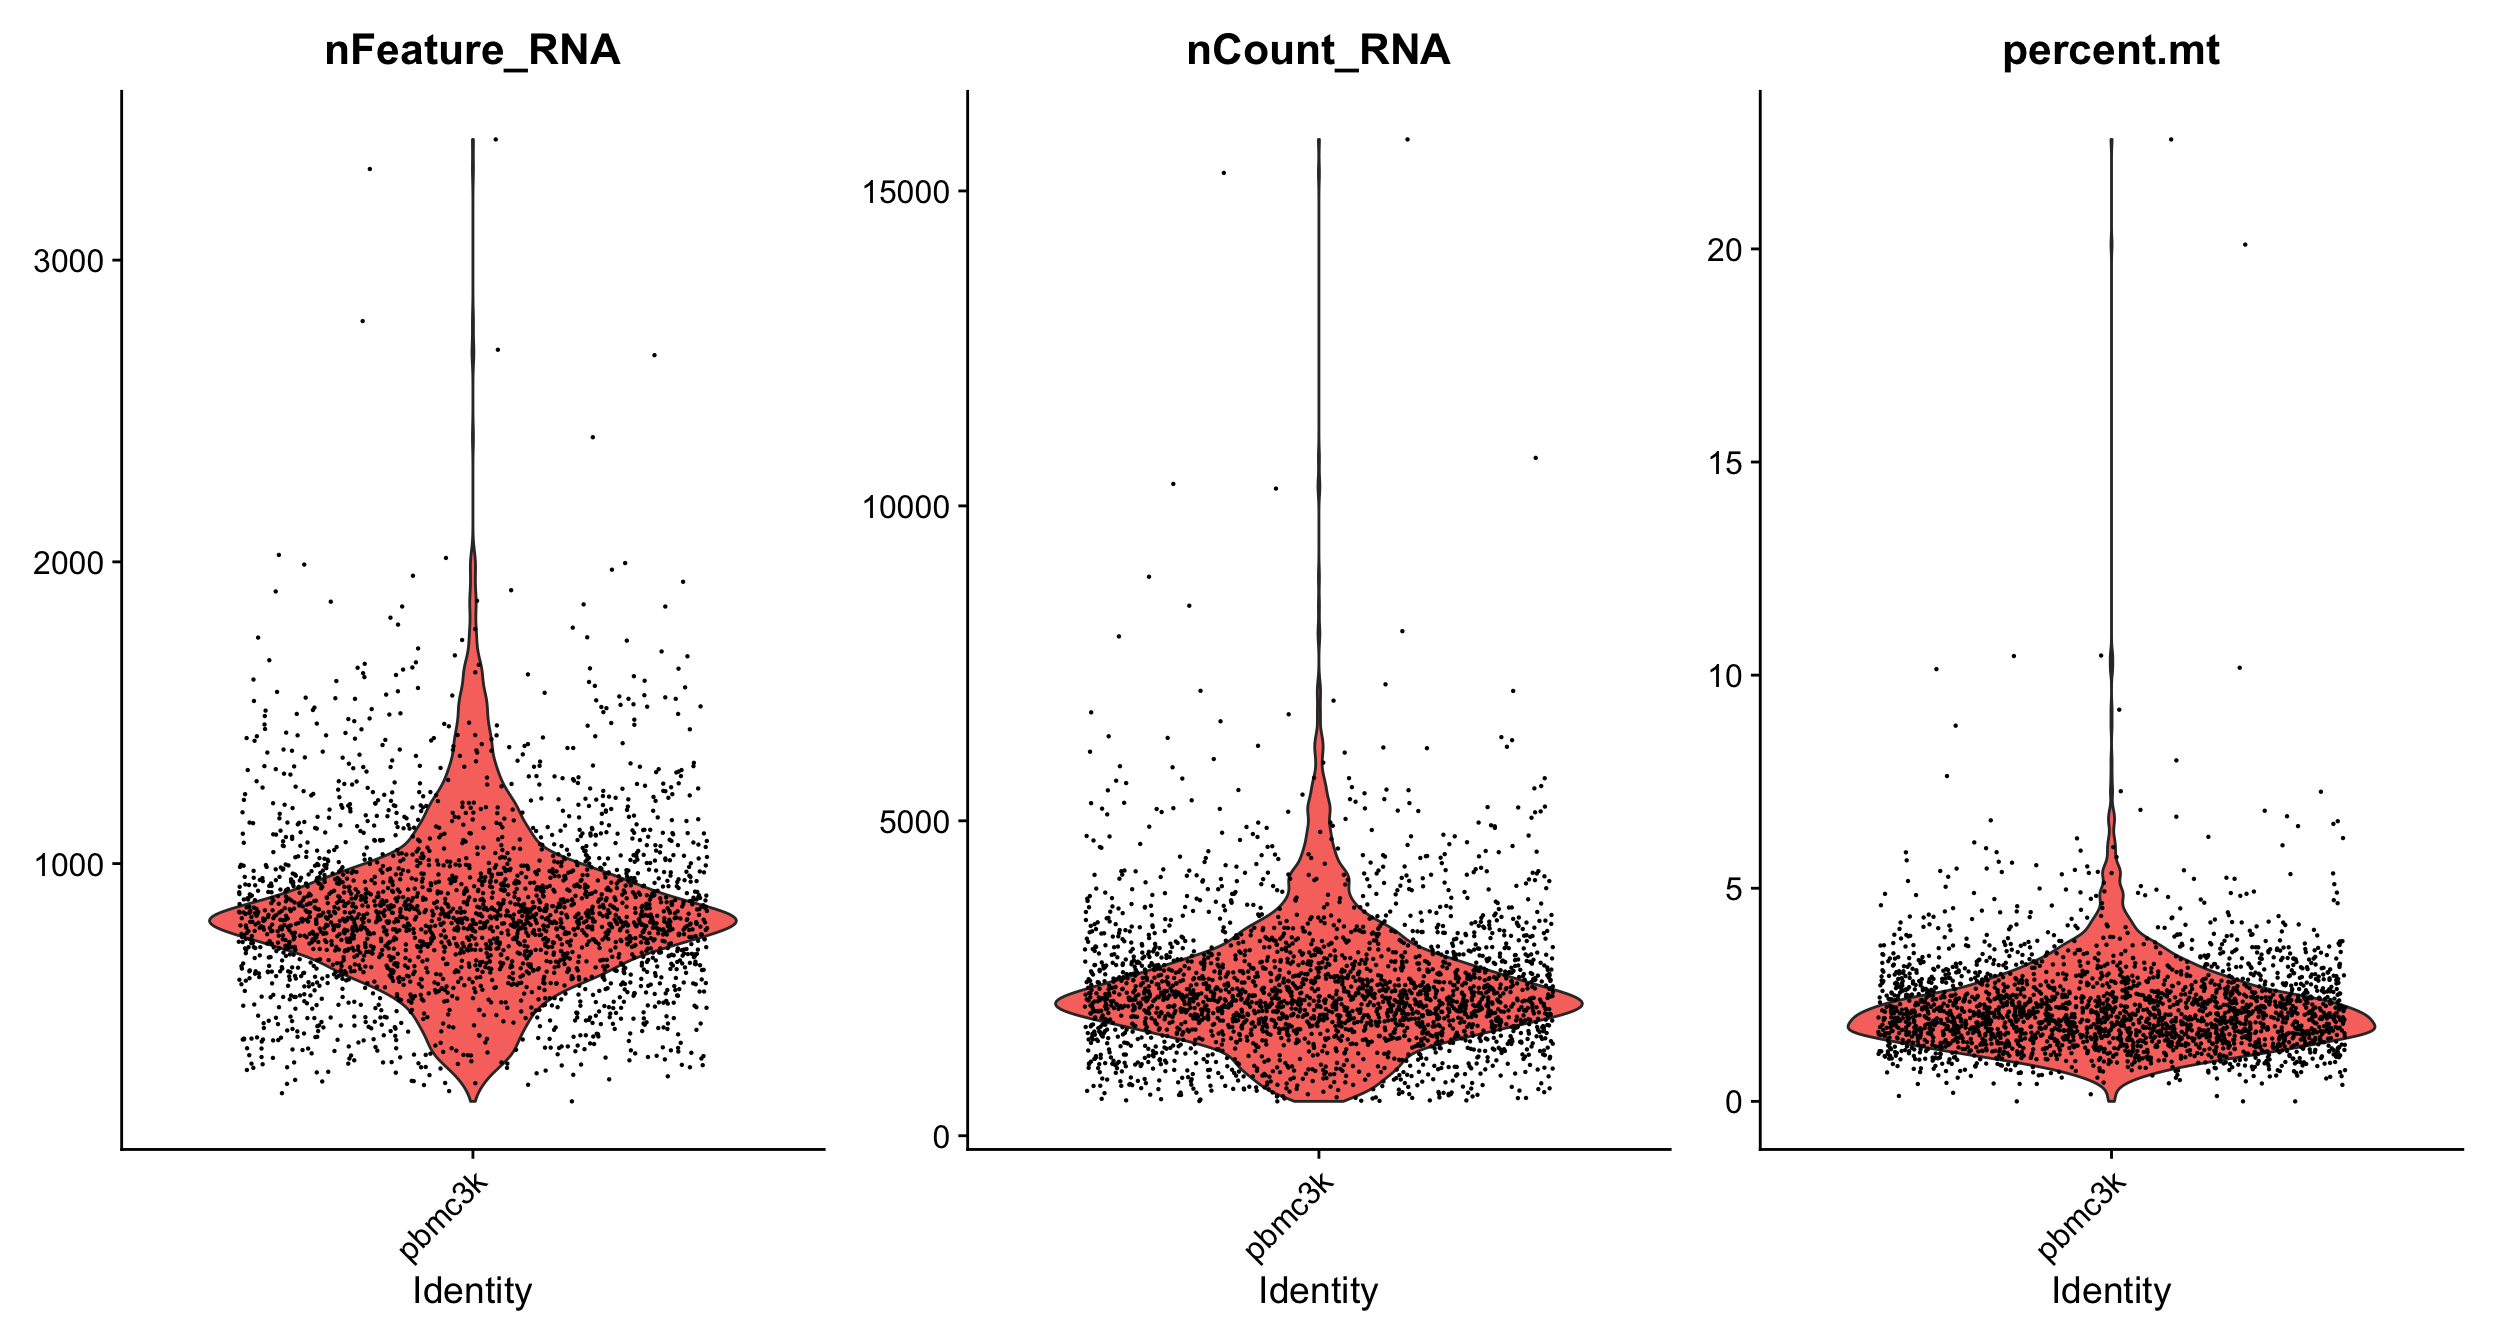
\includegraphics{scRNAseqInR_Doco_files/figure-latex/qc2-1.pdf}

\begin{Shaded}
\begin{Highlighting}[]
\CommentTok{\# FeatureScatter is typically used to visualize feature{-}feature relationships, }
\CommentTok{\# but can be used for anything calculated by the object, }
\CommentTok{\# i.e. columns in object metadata, PC scores etc.}
\NormalTok{plot1 }\OtherTok{\textless{}{-}} \FunctionTok{FeatureScatter}\NormalTok{(pbmc, }\AttributeTok{feature1 =} \StringTok{"nCount\_RNA"}\NormalTok{, }\AttributeTok{feature2 =} \StringTok{"percent.mt"}\NormalTok{) }
\NormalTok{plot2 }\OtherTok{\textless{}{-}} \FunctionTok{FeatureScatter}\NormalTok{(pbmc, }\AttributeTok{feature1 =} \StringTok{"nCount\_RNA"}\NormalTok{, }\AttributeTok{feature2 =} \StringTok{"nFeature\_RNA"}\NormalTok{) }
\NormalTok{plot1 }\SpecialCharTok{+}\NormalTok{ plot2}
\end{Highlighting}
\end{Shaded}

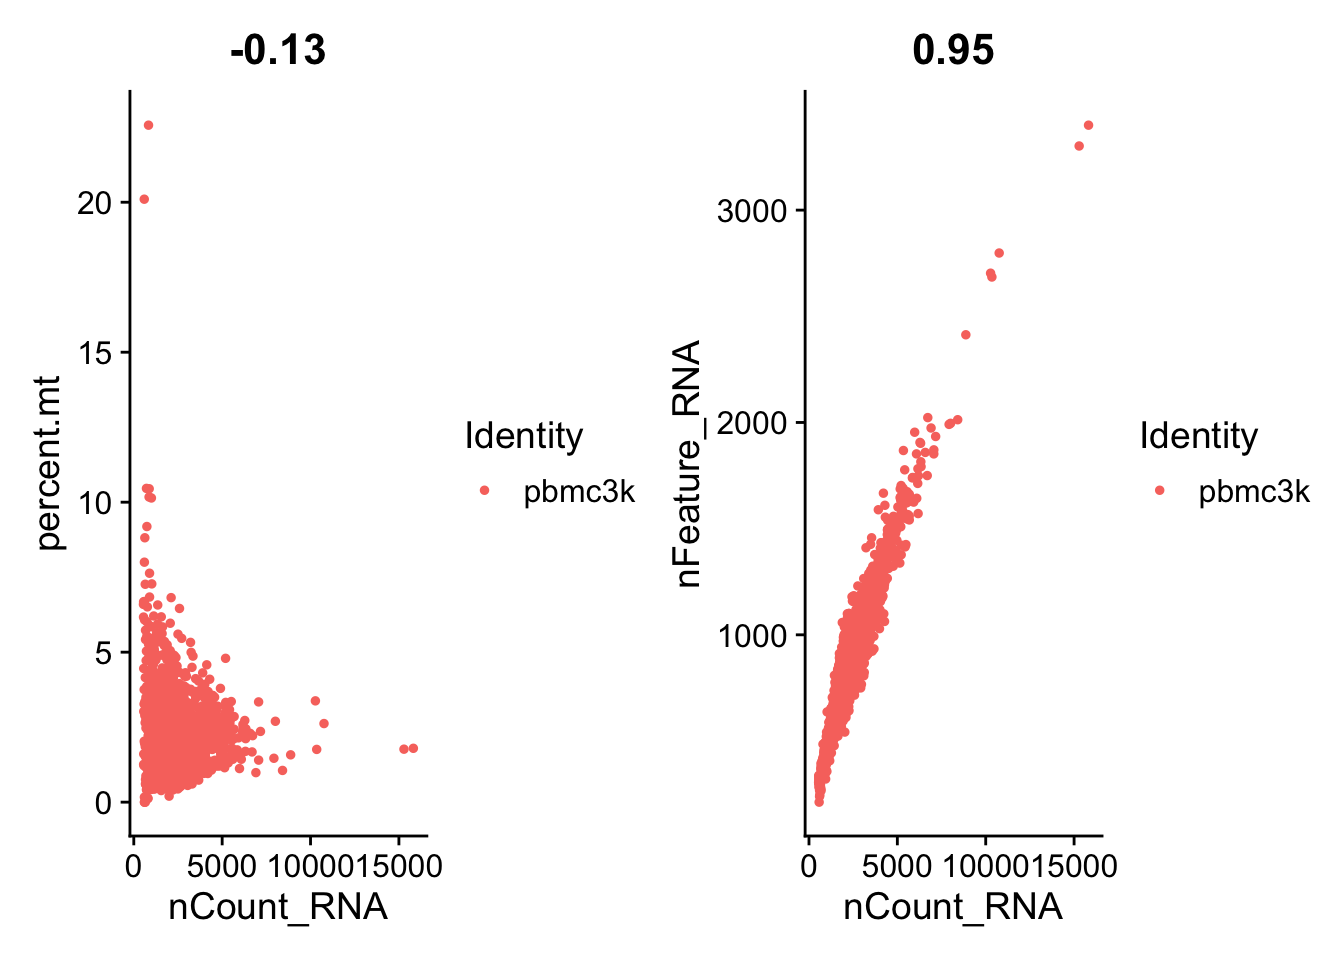
\includegraphics{scRNAseqInR_Doco_files/figure-latex/qc2-2.pdf}

Lets look at the number of features (genes) to the percent mitochondrial genes plot.

\begin{Shaded}
\begin{Highlighting}[]
\NormalTok{plot3 }\OtherTok{\textless{}{-}} \FunctionTok{FeatureScatter}\NormalTok{(pbmc, }\AttributeTok{feature1 =} \StringTok{"nFeature\_RNA"}\NormalTok{, }\AttributeTok{feature2 =} \StringTok{"percent.mt"}\NormalTok{) }
\NormalTok{plot3}
\end{Highlighting}
\end{Shaded}

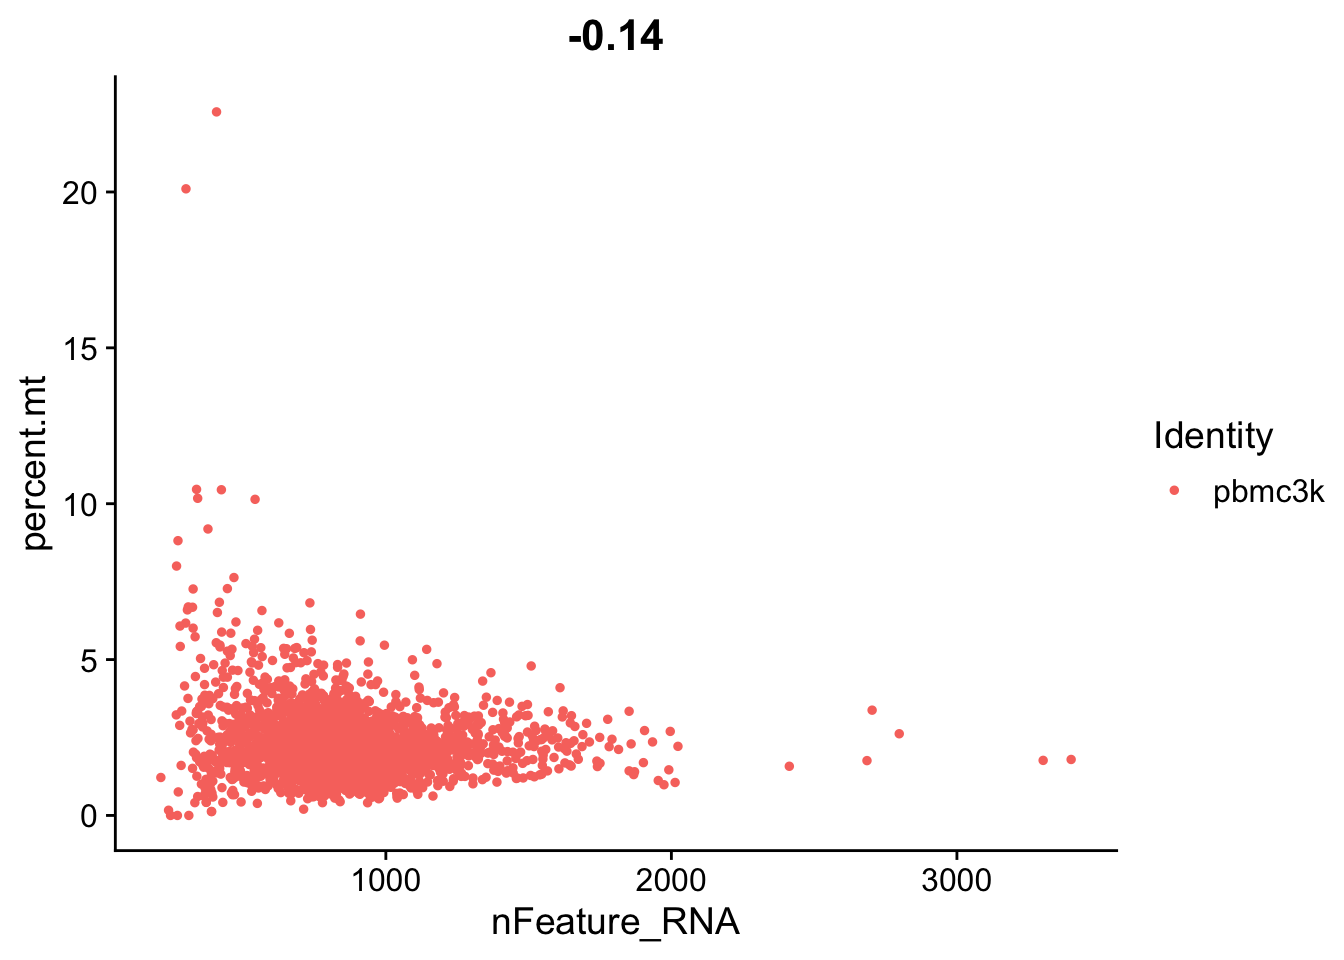
\includegraphics{scRNAseqInR_Doco_files/figure-latex/unnamed-chunk-17-1.pdf}

Okay we are happy with our thresholds for mitochondrial percentage in cells, lets apply them and subset our data. This will remove the cells we think are of poor quality.

\begin{Shaded}
\begin{Highlighting}[]
\NormalTok{pbmc }\OtherTok{\textless{}{-}} \FunctionTok{subset}\NormalTok{(pbmc, }\AttributeTok{subset =}\NormalTok{ nFeature\_RNA }\SpecialCharTok{\textgreater{}} \DecValTok{200} \SpecialCharTok{\&}\NormalTok{ nFeature\_RNA }\SpecialCharTok{\textless{}} \DecValTok{2500} \SpecialCharTok{\&}\NormalTok{ percent.mt }\SpecialCharTok{\textless{}} \DecValTok{5}\NormalTok{)}
\end{Highlighting}
\end{Shaded}

Lets replot the feature scatters and see what they look like.

\begin{Shaded}
\begin{Highlighting}[]
\NormalTok{plot5 }\OtherTok{\textless{}{-}} \FunctionTok{FeatureScatter}\NormalTok{(pbmc, }\AttributeTok{feature1 =} \StringTok{"nCount\_RNA"}\NormalTok{, }\AttributeTok{feature2 =} \StringTok{"percent.mt"}\NormalTok{) }
\NormalTok{plot6 }\OtherTok{\textless{}{-}} \FunctionTok{FeatureScatter}\NormalTok{(pbmc, }\AttributeTok{feature1 =} \StringTok{"nCount\_RNA"}\NormalTok{, }\AttributeTok{feature2 =} \StringTok{"nFeature\_RNA"}\NormalTok{) }
\NormalTok{plot5 }\SpecialCharTok{+}\NormalTok{ plot6}
\end{Highlighting}
\end{Shaded}

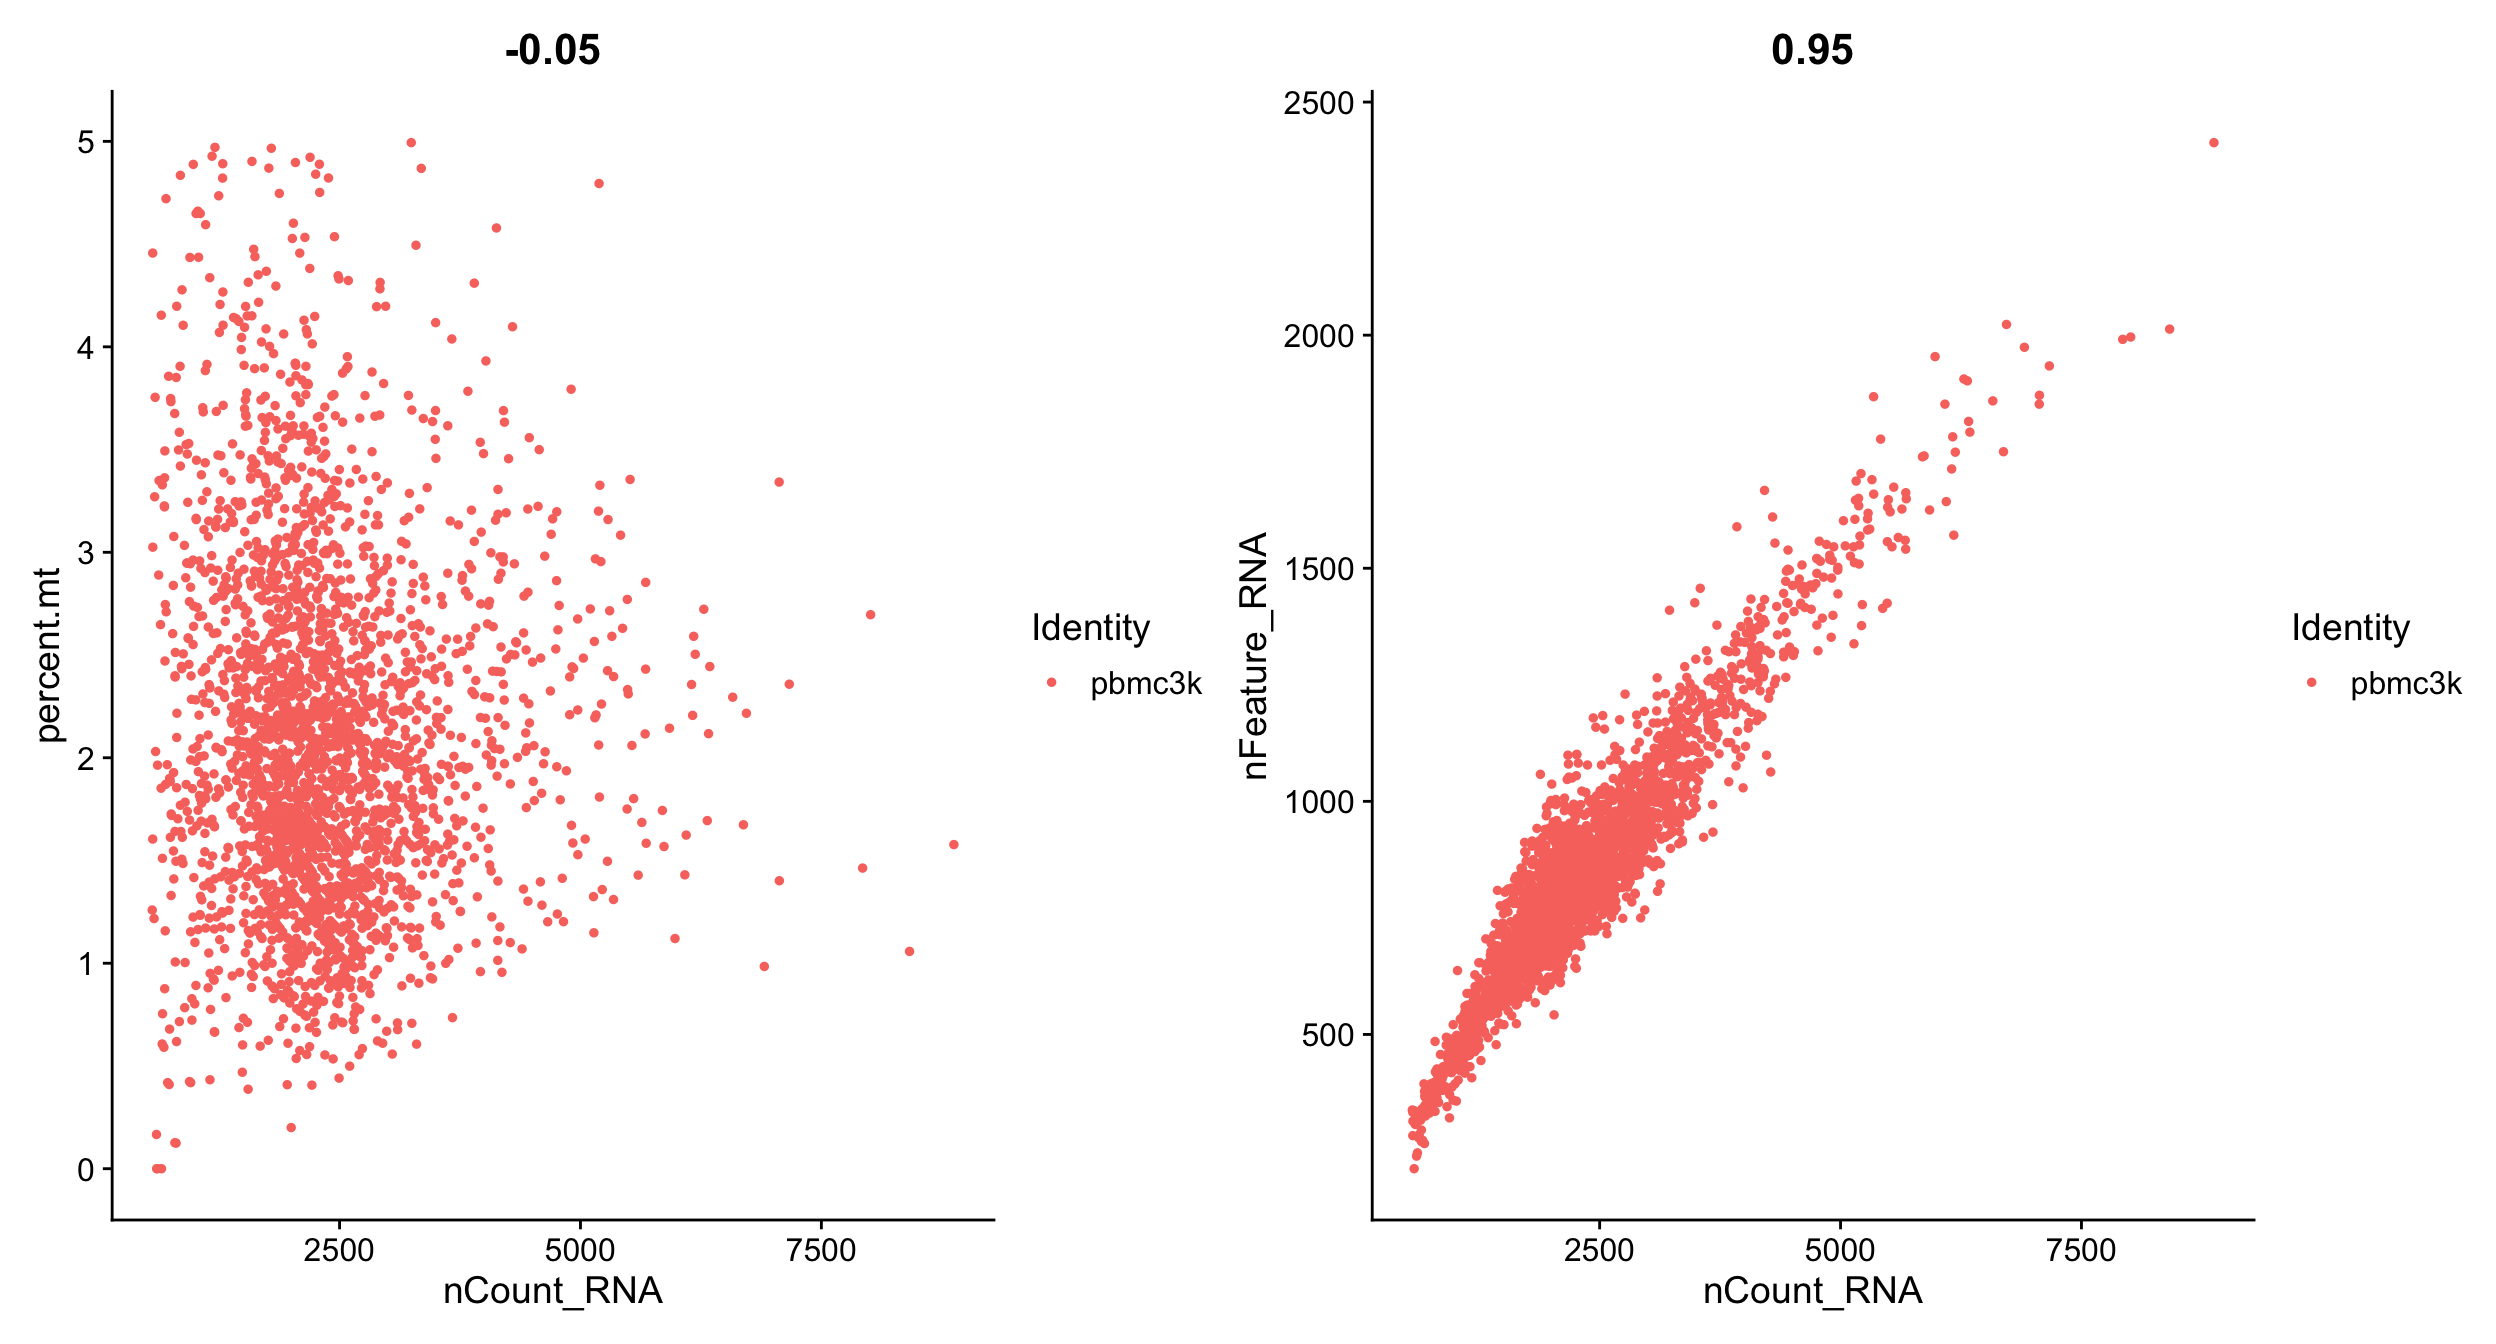
\includegraphics{scRNAseqInR_Doco_files/figure-latex/qc2_sidebar-1.pdf}

\hypertarget{challenge-filter-the-cells}{%
\subsubsection*{Challenge: Filter the cells}\label{challenge-filter-the-cells}}
\addcontentsline{toc}{subsubsection}{Challenge: Filter the cells}

Apply the filtering thresolds defined above.

\begin{itemize}
\tightlist
\item
  How many cells survived filtering?
\end{itemize}

The PBMC3k dataset we're working with in this tutorial is quite old. There are a number of other example datasets available from the 10X website, including \href{https://www.10xgenomics.com/resources/datasets/10k-human-pbmcs-3-v3-1-chromium-x-with-intronic-reads-3-1-high}{this one} - published in 2022, sequencing 10k PBMCs with a newer chemistry and counting method.

\begin{itemize}
\tightlist
\item
  What thresholds would you chose to apply to this modern dataset?
\end{itemize}

\begin{Shaded}
\begin{Highlighting}[]
\NormalTok{pbmc10k\_unfiltered }\OtherTok{\textless{}{-}} \FunctionTok{readRDS}\NormalTok{(}\StringTok{"data/10k\_PBMC\_v3.1ChromiumX\_Intronic.rds"}\NormalTok{)}
\FunctionTok{VlnPlot}\NormalTok{(pbmc10k\_unfiltered, }\AttributeTok{features =} \FunctionTok{c}\NormalTok{(}\StringTok{"nFeature\_RNA"}\NormalTok{, }\StringTok{"nCount\_RNA"}\NormalTok{), }\AttributeTok{ncol =} \DecValTok{2}\NormalTok{)}
\end{Highlighting}
\end{Shaded}

\hypertarget{norm}{%
\chapter{Normalisation}\label{norm}}

After removing unwanted cells from the dataset, the next step is to normalize the data. By default, we employ a global-scaling normalization method ``LogNormalize'' that normalizes the feature expression measurements for each cell by the total expression, multiplies this by a scale factor (10,000 by default), and log-transforms the result. Normalized values are stored in \texttt{pbmc\$RNA@data}.

\begin{Shaded}
\begin{Highlighting}[]
\NormalTok{pbmc }\OtherTok{\textless{}{-}} \FunctionTok{NormalizeData}\NormalTok{(pbmc, }\AttributeTok{normalization.method =} \StringTok{"LogNormalize"}\NormalTok{, }\AttributeTok{scale.factor =} \FloatTok{1e4}\NormalTok{)}
\end{Highlighting}
\end{Shaded}

For clarity, in this previous line of code (and in future commands), we provide the default values for certain parameters in the function call. However, this isn't required and the same behavior can be achieved with:

\begin{Shaded}
\begin{Highlighting}[]
\NormalTok{pbmc }\OtherTok{\textless{}{-}} \FunctionTok{NormalizeData}\NormalTok{(pbmc)}
\end{Highlighting}
\end{Shaded}

\hypertarget{reducedims}{%
\chapter{PCAs and UMAPs}\label{reducedims}}

\hypertarget{identification-of-highly-variable-features-feature-selection}{%
\section{Identification of highly variable features (feature selection)}\label{identification-of-highly-variable-features-feature-selection}}

We next calculate a subset of features that exhibit high cell-to-cell variation in the dataset (i.e, they are highly expressed in some cells, and lowly expressed in others). We and \href{https://www.nature.com/articles/nmeth.2645}{others} have found that focusing on these genes in downstream analysis helps to highlight biological signal in single-cell datasets.

Our procedure in Seurat is described in detail \href{https://doi.org/10.1016/j.cell.2019.05.031}{here}, and improves on previous versions by directly modeling the mean-variance relationship inherent in single-cell data, and is implemented in the \texttt{FindVariableFeatures()} function. By default, we return 2,000 features per dataset. These will be used in downstream analysis, like PCA.

\begin{Shaded}
\begin{Highlighting}[]
\NormalTok{pbmc }\OtherTok{\textless{}{-}} \FunctionTok{FindVariableFeatures}\NormalTok{(pbmc, }\AttributeTok{selection.method =} \StringTok{\textquotesingle{}vst\textquotesingle{}}\NormalTok{, }\AttributeTok{nfeatures =} \DecValTok{2000}\NormalTok{)}
\CommentTok{\# Identify the 10 most highly variable genes}
\NormalTok{top10 }\OtherTok{\textless{}{-}} \FunctionTok{head}\NormalTok{(}\FunctionTok{VariableFeatures}\NormalTok{(pbmc), }\DecValTok{10}\NormalTok{)}
\CommentTok{\# plot variable features with and without labels}
\NormalTok{plot1 }\OtherTok{\textless{}{-}} \FunctionTok{VariableFeaturePlot}\NormalTok{(pbmc)}
\NormalTok{plot2 }\OtherTok{\textless{}{-}} \FunctionTok{LabelPoints}\NormalTok{(}\AttributeTok{plot =}\NormalTok{ plot1, }\AttributeTok{points =}\NormalTok{ top10, }\AttributeTok{repel =} \ConstantTok{TRUE}\NormalTok{)}
\CommentTok{\#\textgreater{} When using repel, set xnudge and ynudge to 0 for optimal results}
\NormalTok{plot1 }\SpecialCharTok{+}\NormalTok{ plot2}
\CommentTok{\#\textgreater{} Warning: Transformation introduced infinite values in continuous}
\CommentTok{\#\textgreater{} x{-}axis}
\CommentTok{\#\textgreater{} Transformation introduced infinite values in continuous}
\CommentTok{\#\textgreater{} x{-}axis}
\end{Highlighting}
\end{Shaded}

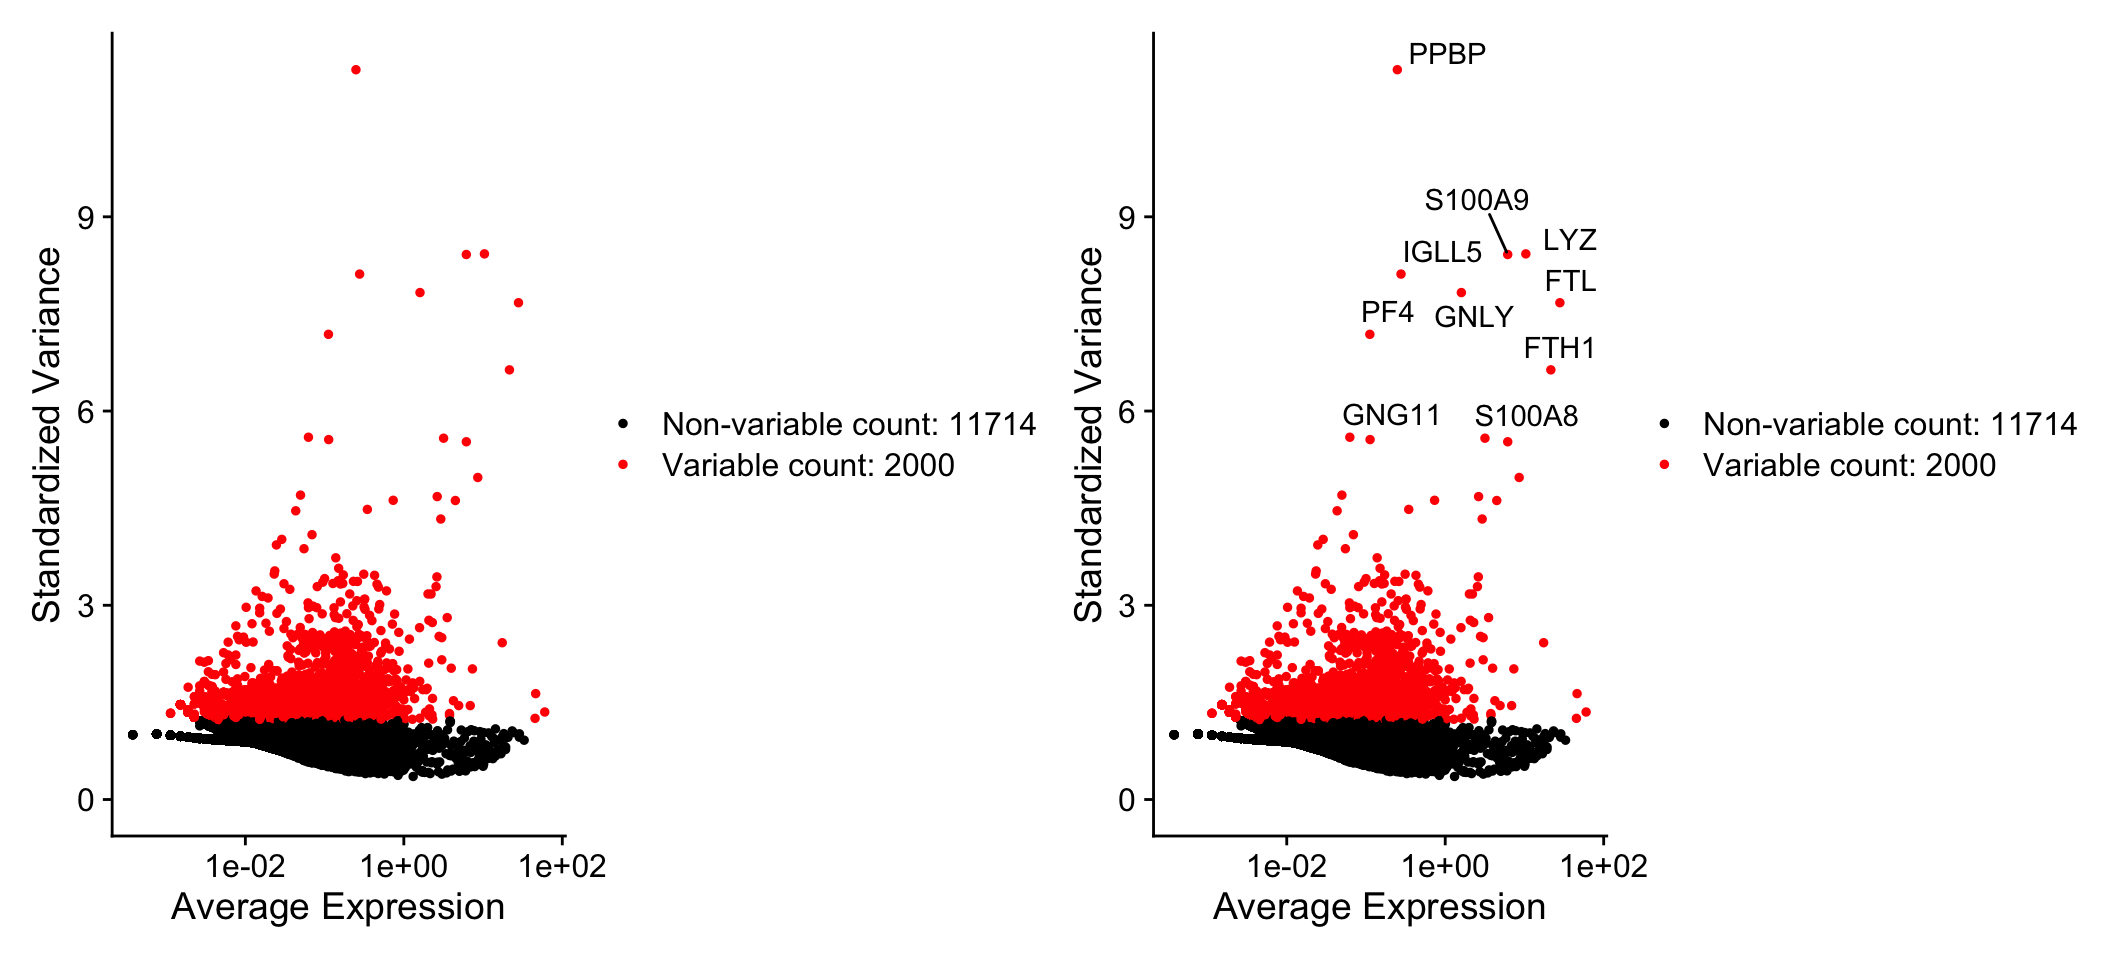
\includegraphics{scRNAseqInR_Doco_files/figure-latex/var_features-1.pdf}

\hypertarget{scaling-the-data}{%
\section{Scaling the data}\label{scaling-the-data}}

Next, we apply a linear transformation (`scaling') that is a standard pre-processing step prior to dimensional reduction techniques like PCA. The \texttt{ScaleData()} function:

\begin{itemize}
\tightlist
\item
  Shifts the expression of each gene, so that the mean expression across cells is 0
\item
  Scales the expression of each gene, so that the variance across cells is 1

  \begin{itemize}
  \tightlist
  \item
    This step gives equal weight in downstream analyses, so that highly-expressed genes do not dominate
  \end{itemize}
\item
  The results of this are stored in \texttt{pbmc\$RNA@scale.data}
\end{itemize}

\begin{Shaded}
\begin{Highlighting}[]
\NormalTok{all.genes }\OtherTok{\textless{}{-}} \FunctionTok{rownames}\NormalTok{(pbmc)}
\NormalTok{pbmc }\OtherTok{\textless{}{-}} \FunctionTok{ScaleData}\NormalTok{(pbmc, }\AttributeTok{features =}\NormalTok{ all.genes)}
\CommentTok{\#\textgreater{} Centering and scaling data matrix}
\end{Highlighting}
\end{Shaded}

\textbf{This step takes too long! Can I make it faster?}

Scaling is an essential step in the Seurat workflow, but only on genes that will be used as input to PCA. Therefore, the default in \texttt{ScaleData()} is only to perform scaling on the previously identified variable features (2,000 by default). To do this, omit the \texttt{features} argument in the previous function call, i.e.

\begin{Shaded}
\begin{Highlighting}[]
\CommentTok{\# pbmc \textless{}{-} ScaleData(pbmc)}
\end{Highlighting}
\end{Shaded}

Your PCA and clustering results will be unaffected. However, Seurat heatmaps (produced as shown below with \texttt{DoHeatmap()}) require genes in the heatmap to be scaled, to make sure highly-expressed genes don't dominate the heatmap. To make sure we don't leave any genes out of the heatmap later, we are scaling all genes in this tutorial.

~

\textbf{How can I remove unwanted sources of variation, as in Seurat v2?}

In \texttt{Seurat\ v2} we also use the \texttt{ScaleData()} function to remove unwanted sources of variation from a single-cell dataset. For example, we could `regress out' heterogeneity associated with (for example) cell cycle stage, or mitochondrial contamination. These features are still supported in \texttt{ScaleData()} in \texttt{Seurat\ v3}, i.e.:

\begin{Shaded}
\begin{Highlighting}[]
\CommentTok{\# pbmc \textless{}{-} ScaleData(pbmc, vars.to.regress = \textquotesingle{}percent.mt\textquotesingle{})}
\end{Highlighting}
\end{Shaded}

However, particularly for advanced users who would like to use this functionality, we strongly recommend the use of our new normalization workflow, \texttt{SCTransform()}. The method is described in our \href{https://genomebiology.biomedcentral.com/articles/10.1186/s13059-019-1874-1}{paper}, with a separate vignette using Seurat v3 \href{sctransform_vignette.html}{here}. As with \texttt{ScaleData()}, the function \texttt{SCTransform()} also includes a \texttt{vars.to.regress} parameter.

~

\begin{center}\rule{0.5\linewidth}{0.5pt}\end{center}

\hypertarget{perform-linear-dimensional-reduction}{%
\section{Perform linear dimensional reduction}\label{perform-linear-dimensional-reduction}}

Next we perform PCA on the scaled data. By default, only the previously determined variable features are used as input, but can be defined using \texttt{features} argument if you wish to choose a different subset.

\begin{Shaded}
\begin{Highlighting}[]
\NormalTok{pbmc }\OtherTok{\textless{}{-}} \FunctionTok{RunPCA}\NormalTok{(pbmc, }\AttributeTok{features =} \FunctionTok{VariableFeatures}\NormalTok{(}\AttributeTok{object =}\NormalTok{ pbmc))}
\CommentTok{\#\textgreater{} PC\_ 1 }
\CommentTok{\#\textgreater{} Positive:  CST3, TYROBP, LST1, AIF1, FTL, FTH1, LYZ, FCN1, S100A9, TYMP }
\CommentTok{\#\textgreater{}     FCER1G, CFD, LGALS1, S100A8, CTSS, LGALS2, SERPINA1, IFITM3, SPI1, CFP }
\CommentTok{\#\textgreater{}     PSAP, IFI30, SAT1, COTL1, S100A11, NPC2, GRN, LGALS3, GSTP1, PYCARD }
\CommentTok{\#\textgreater{} Negative:  MALAT1, LTB, IL32, IL7R, CD2, B2M, ACAP1, CD27, STK17A, CTSW }
\CommentTok{\#\textgreater{}     CD247, GIMAP5, AQP3, CCL5, SELL, TRAF3IP3, GZMA, MAL, CST7, ITM2A }
\CommentTok{\#\textgreater{}     MYC, GIMAP7, HOPX, BEX2, LDLRAP1, GZMK, ETS1, ZAP70, TNFAIP8, RIC3 }
\CommentTok{\#\textgreater{} PC\_ 2 }
\CommentTok{\#\textgreater{} Positive:  CD79A, MS4A1, TCL1A, HLA{-}DQA1, HLA{-}DQB1, HLA{-}DRA, LINC00926, CD79B, HLA{-}DRB1, CD74 }
\CommentTok{\#\textgreater{}     HLA{-}DMA, HLA{-}DPB1, HLA{-}DQA2, CD37, HLA{-}DRB5, HLA{-}DMB, HLA{-}DPA1, FCRLA, HVCN1, LTB }
\CommentTok{\#\textgreater{}     BLNK, P2RX5, IGLL5, IRF8, SWAP70, ARHGAP24, FCGR2B, SMIM14, PPP1R14A, C16orf74 }
\CommentTok{\#\textgreater{} Negative:  NKG7, PRF1, CST7, GZMB, GZMA, FGFBP2, CTSW, GNLY, B2M, SPON2 }
\CommentTok{\#\textgreater{}     CCL4, GZMH, FCGR3A, CCL5, CD247, XCL2, CLIC3, AKR1C3, SRGN, HOPX }
\CommentTok{\#\textgreater{}     TTC38, APMAP, CTSC, S100A4, IGFBP7, ANXA1, ID2, IL32, XCL1, RHOC }
\CommentTok{\#\textgreater{} PC\_ 3 }
\CommentTok{\#\textgreater{} Positive:  HLA{-}DQA1, CD79A, CD79B, HLA{-}DQB1, HLA{-}DPB1, HLA{-}DPA1, CD74, MS4A1, HLA{-}DRB1, HLA{-}DRA }
\CommentTok{\#\textgreater{}     HLA{-}DRB5, HLA{-}DQA2, TCL1A, LINC00926, HLA{-}DMB, HLA{-}DMA, CD37, HVCN1, FCRLA, IRF8 }
\CommentTok{\#\textgreater{}     PLAC8, BLNK, MALAT1, SMIM14, PLD4, P2RX5, IGLL5, LAT2, SWAP70, FCGR2B }
\CommentTok{\#\textgreater{} Negative:  PPBP, PF4, SDPR, SPARC, GNG11, NRGN, GP9, RGS18, TUBB1, CLU }
\CommentTok{\#\textgreater{}     HIST1H2AC, AP001189.4, ITGA2B, CD9, TMEM40, PTCRA, CA2, ACRBP, MMD, TREML1 }
\CommentTok{\#\textgreater{}     NGFRAP1, F13A1, SEPT5, RUFY1, TSC22D1, MPP1, CMTM5, RP11{-}367G6.3, MYL9, GP1BA }
\CommentTok{\#\textgreater{} PC\_ 4 }
\CommentTok{\#\textgreater{} Positive:  HLA{-}DQA1, CD79B, CD79A, MS4A1, HLA{-}DQB1, CD74, HIST1H2AC, HLA{-}DPB1, PF4, SDPR }
\CommentTok{\#\textgreater{}     TCL1A, HLA{-}DRB1, HLA{-}DPA1, HLA{-}DQA2, PPBP, HLA{-}DRA, LINC00926, GNG11, SPARC, HLA{-}DRB5 }
\CommentTok{\#\textgreater{}     GP9, AP001189.4, CA2, PTCRA, CD9, NRGN, RGS18, CLU, TUBB1, GZMB }
\CommentTok{\#\textgreater{} Negative:  VIM, IL7R, S100A6, IL32, S100A8, S100A4, GIMAP7, S100A10, S100A9, MAL }
\CommentTok{\#\textgreater{}     AQP3, CD2, CD14, FYB, LGALS2, GIMAP4, ANXA1, CD27, FCN1, RBP7 }
\CommentTok{\#\textgreater{}     LYZ, S100A11, GIMAP5, MS4A6A, S100A12, FOLR3, TRABD2A, AIF1, IL8, IFI6 }
\CommentTok{\#\textgreater{} PC\_ 5 }
\CommentTok{\#\textgreater{} Positive:  GZMB, NKG7, S100A8, FGFBP2, GNLY, CCL4, CST7, PRF1, GZMA, SPON2 }
\CommentTok{\#\textgreater{}     GZMH, S100A9, LGALS2, CCL3, CTSW, XCL2, CD14, CLIC3, S100A12, RBP7 }
\CommentTok{\#\textgreater{}     CCL5, MS4A6A, GSTP1, FOLR3, IGFBP7, TYROBP, TTC38, AKR1C3, XCL1, HOPX }
\CommentTok{\#\textgreater{} Negative:  LTB, IL7R, CKB, VIM, MS4A7, AQP3, CYTIP, RP11{-}290F20.3, SIGLEC10, HMOX1 }
\CommentTok{\#\textgreater{}     LILRB2, PTGES3, MAL, CD27, HN1, CD2, GDI2, CORO1B, ANXA5, TUBA1B }
\CommentTok{\#\textgreater{}     FAM110A, ATP1A1, TRADD, PPA1, CCDC109B, ABRACL, CTD{-}2006K23.1, WARS, VMO1, FYB}
\end{Highlighting}
\end{Shaded}

Seurat provides several useful ways of visualizing both cells and features that define the PCA, including \texttt{VizDimReduction()}, \texttt{DimPlot()}, and \texttt{DimHeatmap()}

\begin{Shaded}
\begin{Highlighting}[]
\CommentTok{\# Examine and visualize PCA results a few different ways}
\FunctionTok{print}\NormalTok{(pbmc}\SpecialCharTok{$}\NormalTok{pca, }\AttributeTok{dims =} \DecValTok{1}\SpecialCharTok{:}\DecValTok{5}\NormalTok{, }\AttributeTok{nfeatures =} \DecValTok{5}\NormalTok{)}
\CommentTok{\#\textgreater{} PC\_ 1 }
\CommentTok{\#\textgreater{} Positive:  CST3, TYROBP, LST1, AIF1, FTL }
\CommentTok{\#\textgreater{} Negative:  MALAT1, LTB, IL32, IL7R, CD2 }
\CommentTok{\#\textgreater{} PC\_ 2 }
\CommentTok{\#\textgreater{} Positive:  CD79A, MS4A1, TCL1A, HLA{-}DQA1, HLA{-}DQB1 }
\CommentTok{\#\textgreater{} Negative:  NKG7, PRF1, CST7, GZMB, GZMA }
\CommentTok{\#\textgreater{} PC\_ 3 }
\CommentTok{\#\textgreater{} Positive:  HLA{-}DQA1, CD79A, CD79B, HLA{-}DQB1, HLA{-}DPB1 }
\CommentTok{\#\textgreater{} Negative:  PPBP, PF4, SDPR, SPARC, GNG11 }
\CommentTok{\#\textgreater{} PC\_ 4 }
\CommentTok{\#\textgreater{} Positive:  HLA{-}DQA1, CD79B, CD79A, MS4A1, HLA{-}DQB1 }
\CommentTok{\#\textgreater{} Negative:  VIM, IL7R, S100A6, IL32, S100A8 }
\CommentTok{\#\textgreater{} PC\_ 5 }
\CommentTok{\#\textgreater{} Positive:  GZMB, NKG7, S100A8, FGFBP2, GNLY }
\CommentTok{\#\textgreater{} Negative:  LTB, IL7R, CKB, VIM, MS4A7}
\FunctionTok{VizDimLoadings}\NormalTok{(pbmc, }\AttributeTok{dims =} \DecValTok{1}\SpecialCharTok{:}\DecValTok{2}\NormalTok{, }\AttributeTok{reduction =} \StringTok{\textquotesingle{}pca\textquotesingle{}}\NormalTok{)}
\end{Highlighting}
\end{Shaded}

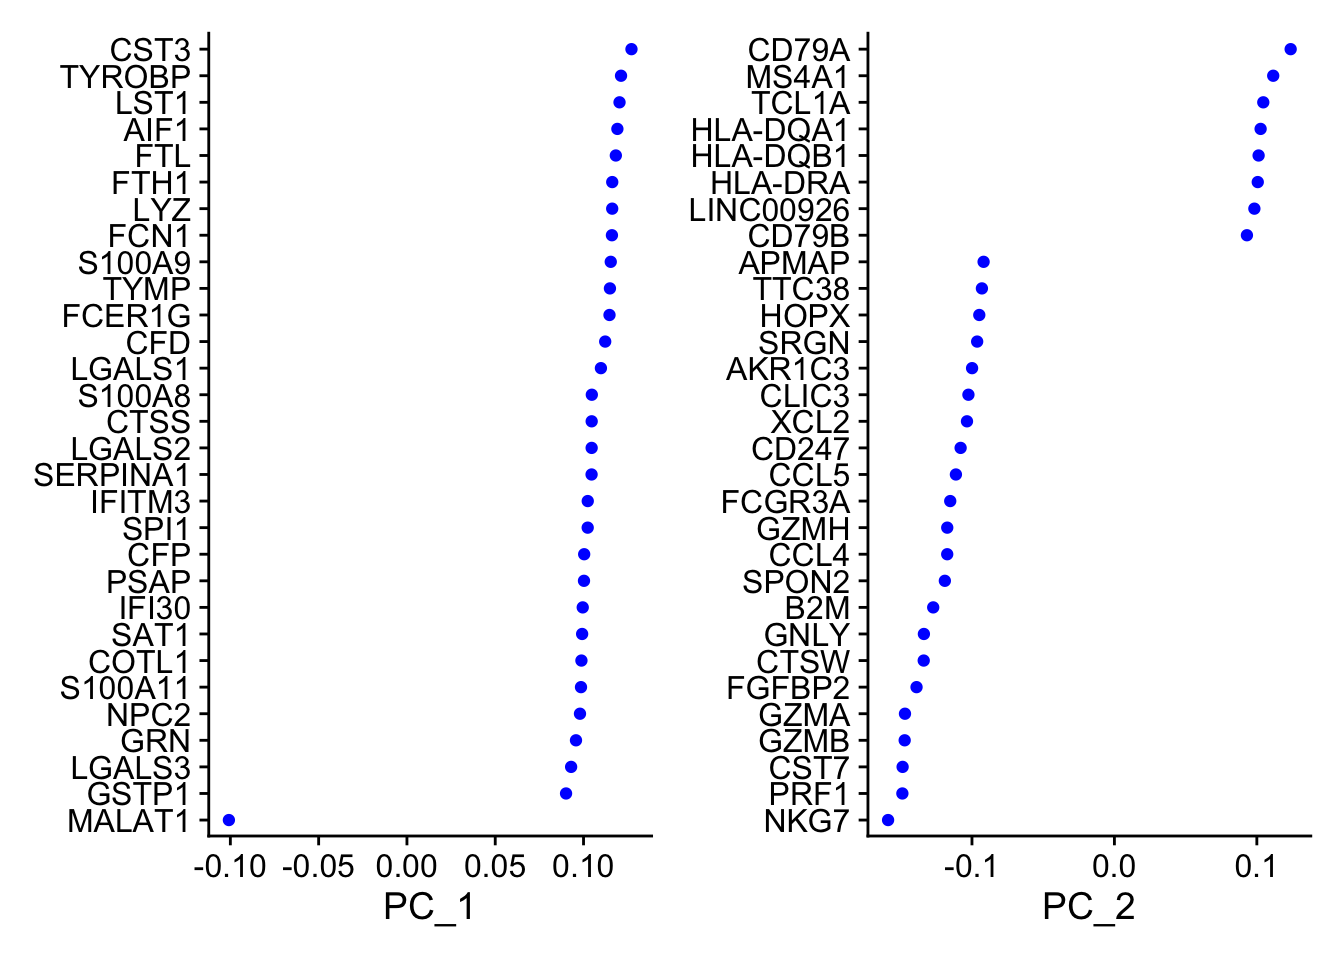
\includegraphics{scRNAseqInR_Doco_files/figure-latex/pca_viz-1.pdf}

\begin{Shaded}
\begin{Highlighting}[]
\FunctionTok{DimPlot}\NormalTok{(pbmc, }\AttributeTok{reduction =} \StringTok{\textquotesingle{}pca\textquotesingle{}}\NormalTok{)}
\end{Highlighting}
\end{Shaded}

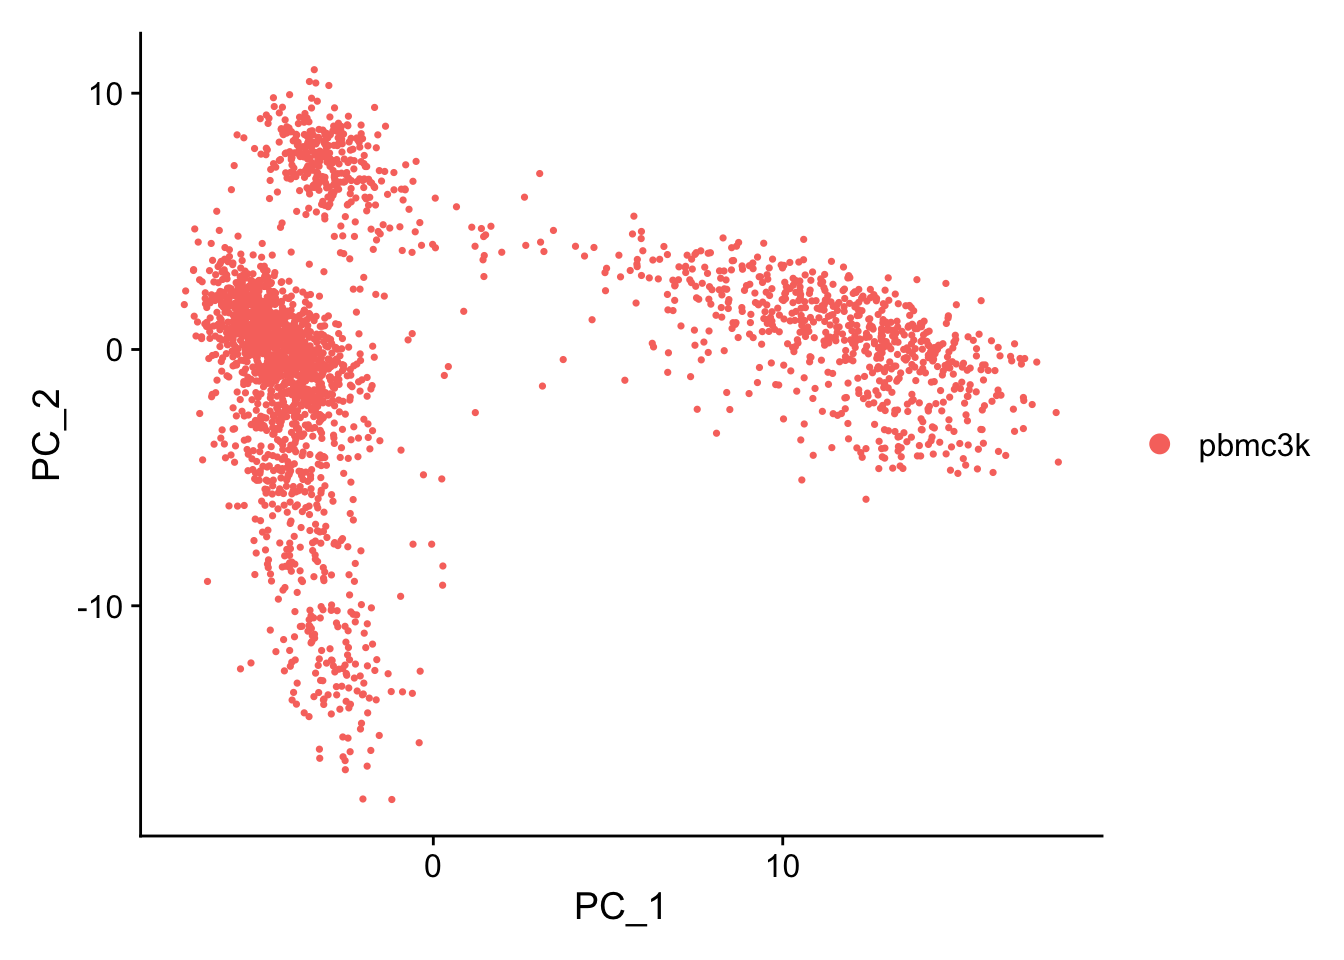
\includegraphics{scRNAseqInR_Doco_files/figure-latex/pca_viz-2.pdf}

In particular \texttt{DimHeatmap()} allows for easy exploration of the primary sources of heterogeneity in a dataset, and can be useful when trying to decide which PCs to include for further downstream analyses. Both cells and features are ordered according to their PCA scores. Setting \texttt{cells} to a number plots the `extreme' cells on both ends of the spectrum, which dramatically speeds plotting for large datasets. Though clearly a supervised analysis, we find this to be a valuable tool for exploring correlated feature sets.

\begin{Shaded}
\begin{Highlighting}[]
\FunctionTok{DimHeatmap}\NormalTok{(pbmc, }\AttributeTok{dims =} \DecValTok{1}\NormalTok{, }\AttributeTok{cells =} \DecValTok{500}\NormalTok{, }\AttributeTok{balanced =} \ConstantTok{TRUE}\NormalTok{)}
\end{Highlighting}
\end{Shaded}

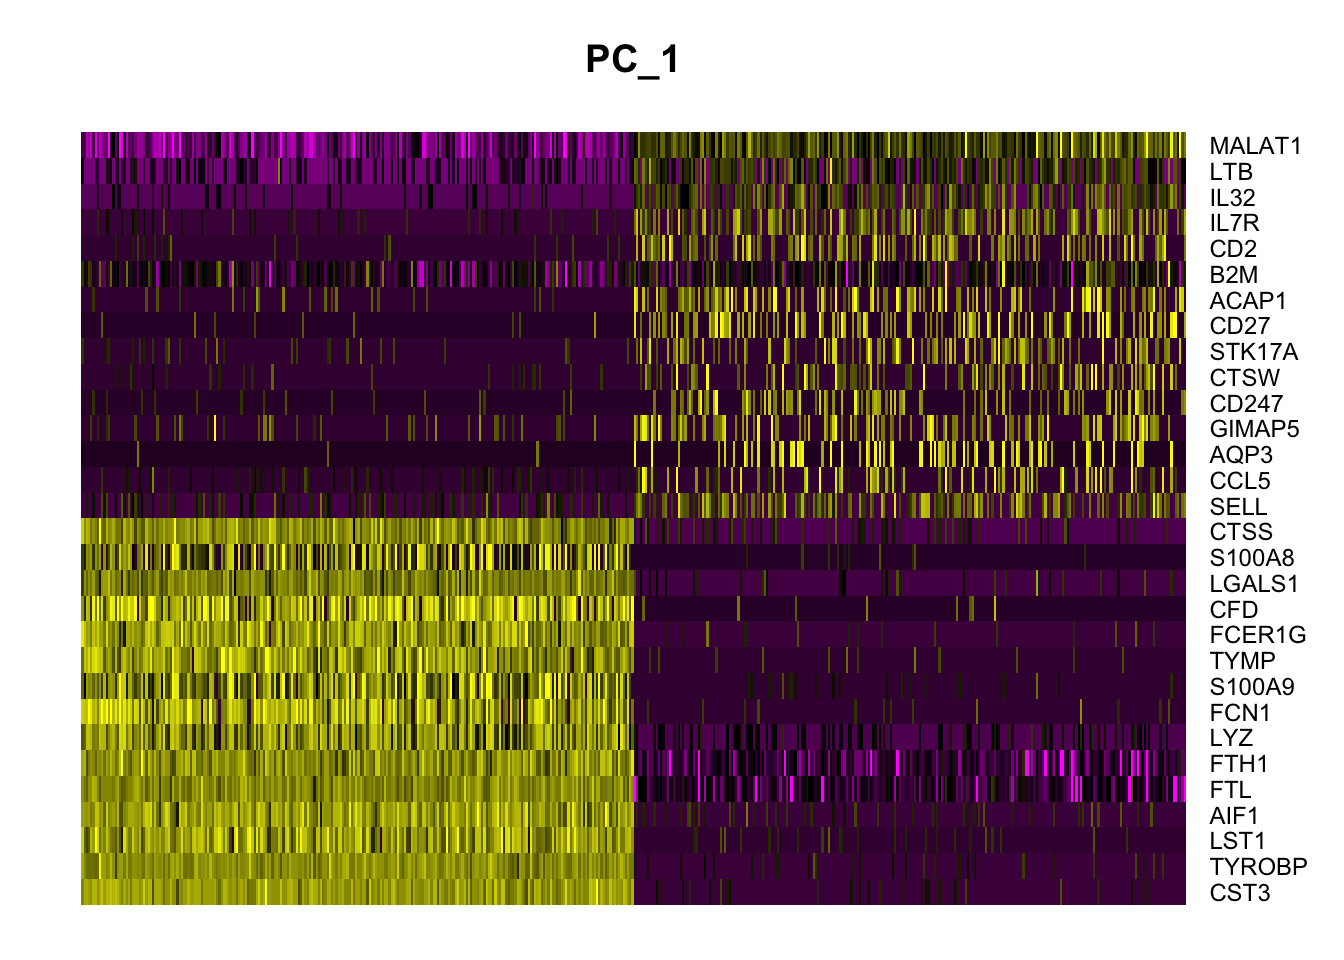
\includegraphics{scRNAseqInR_Doco_files/figure-latex/single-heatmap-1.pdf}

\begin{Shaded}
\begin{Highlighting}[]
\FunctionTok{DimHeatmap}\NormalTok{(pbmc, }\AttributeTok{dims =} \DecValTok{1}\SpecialCharTok{:}\DecValTok{15}\NormalTok{, }\AttributeTok{cells =} \DecValTok{500}\NormalTok{, }\AttributeTok{balanced =} \ConstantTok{TRUE}\NormalTok{)}
\end{Highlighting}
\end{Shaded}

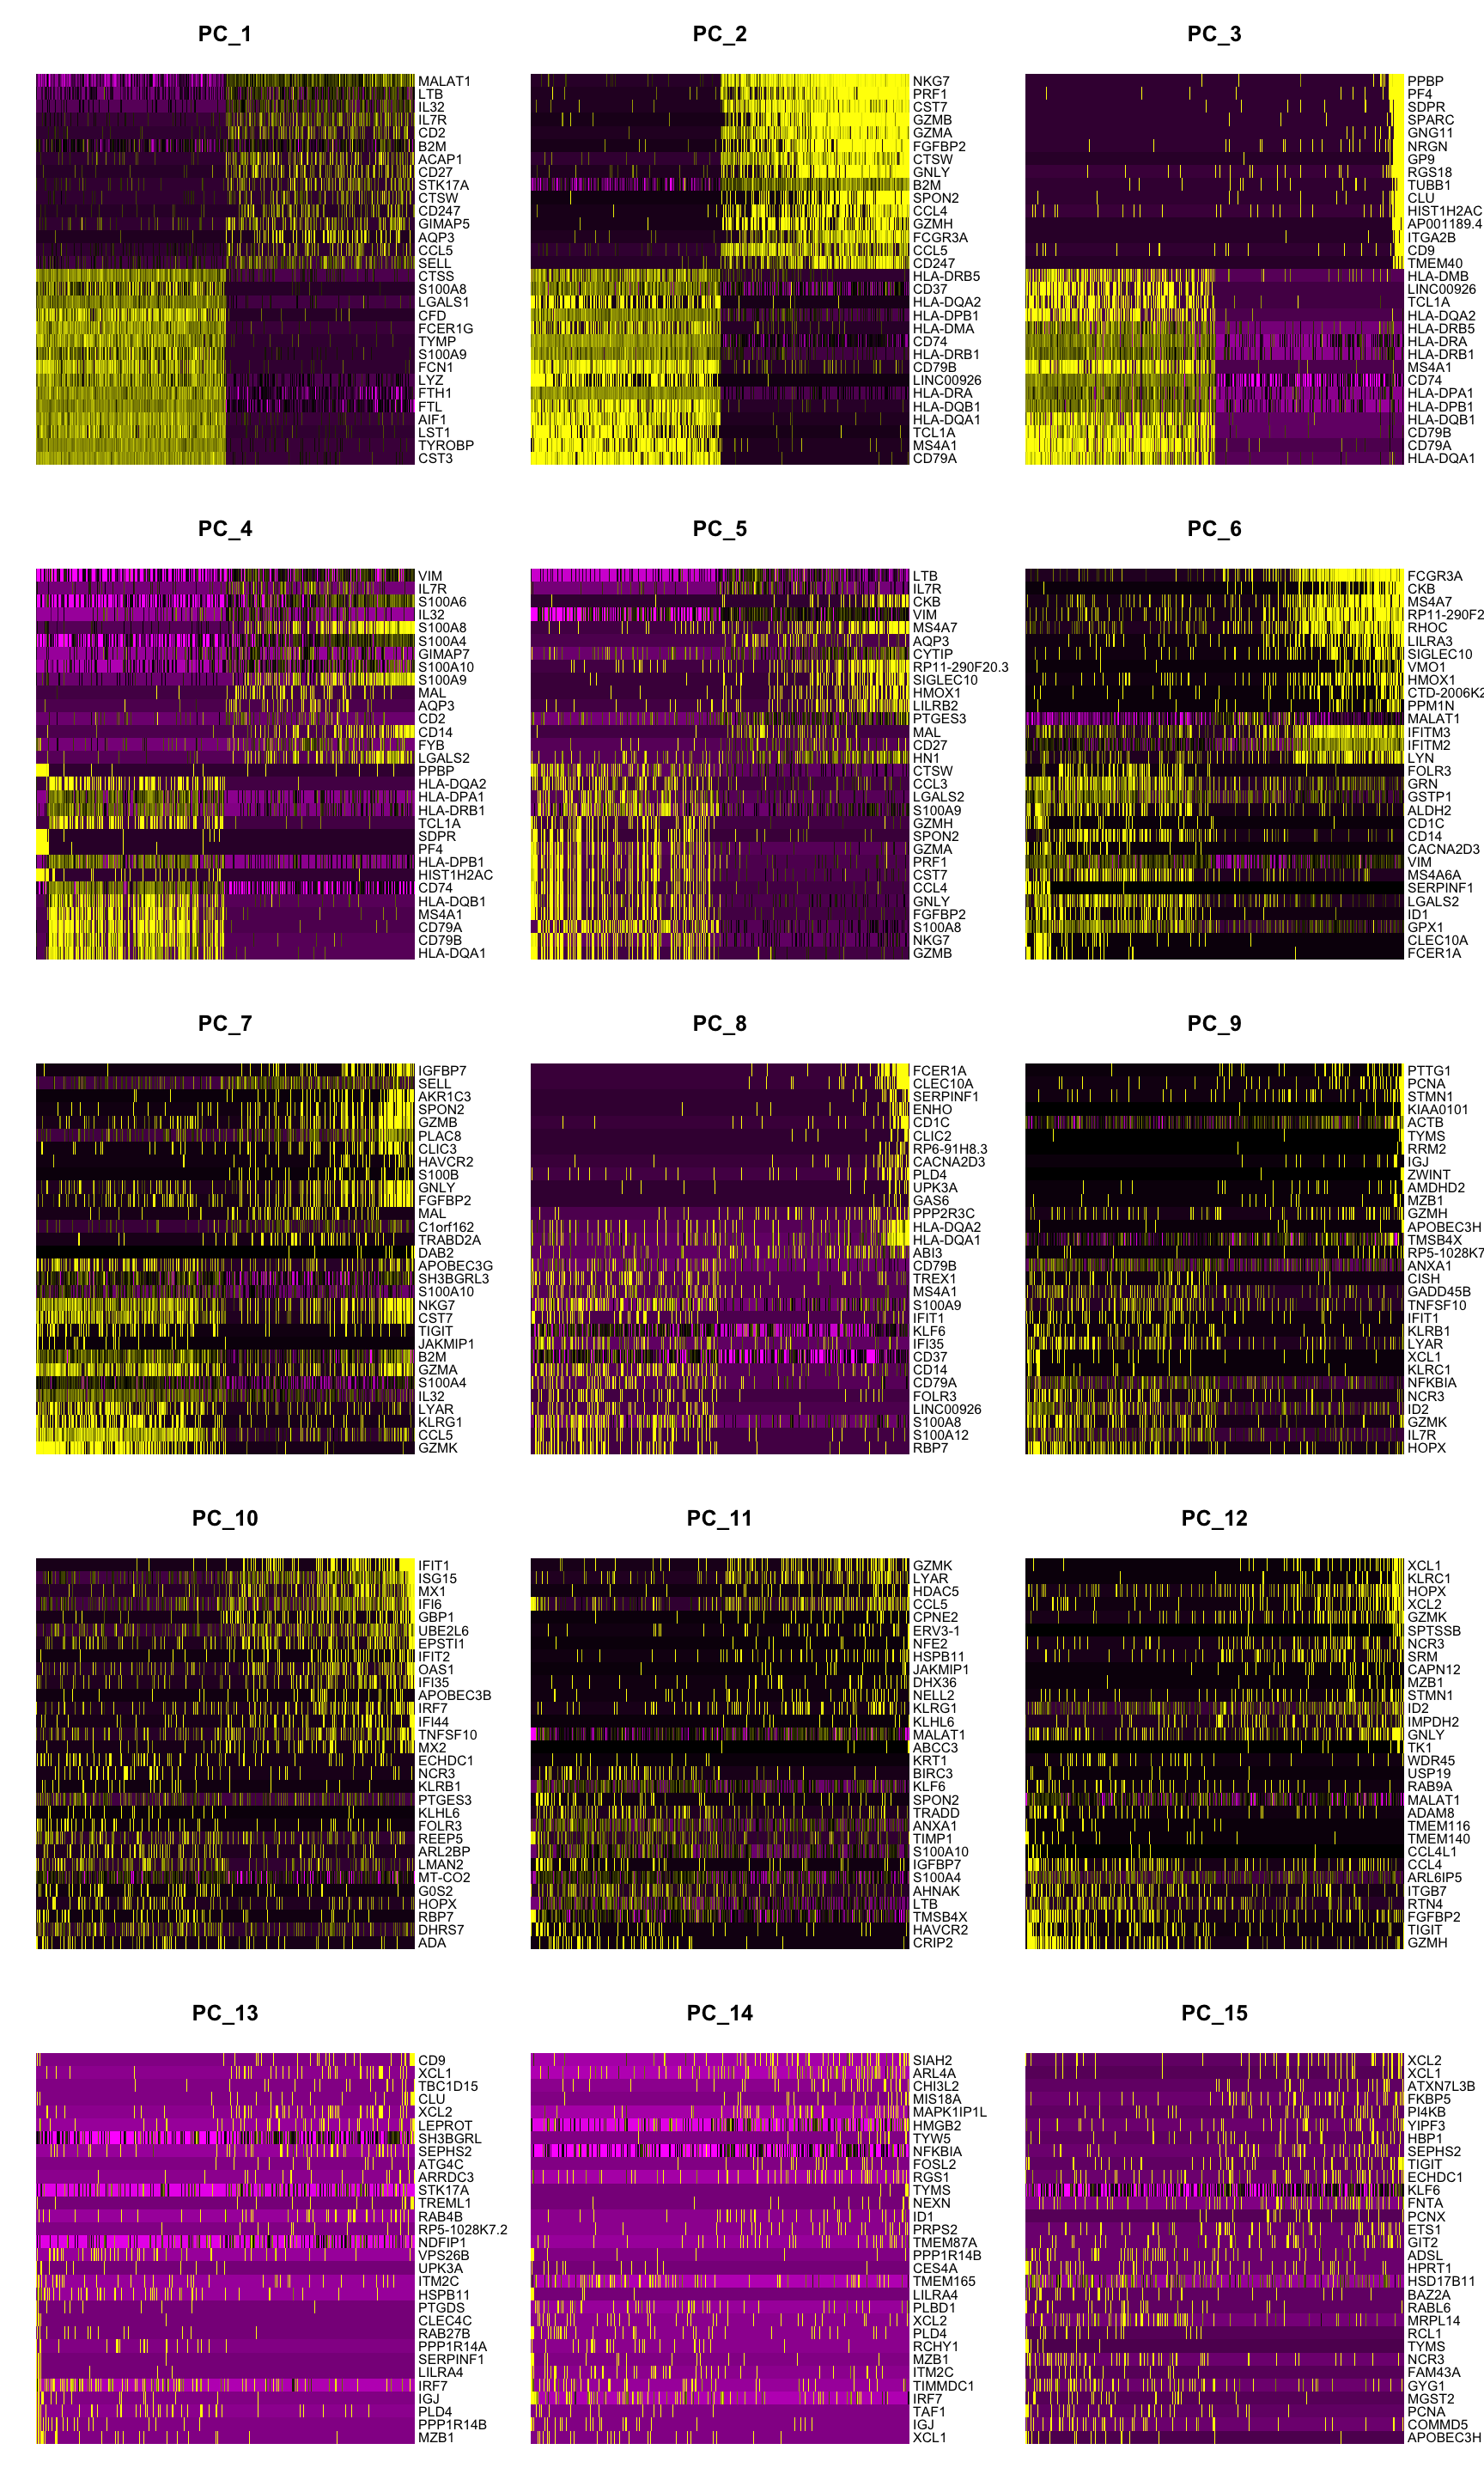
\includegraphics{scRNAseqInR_Doco_files/figure-latex/multi-heatmap-1.pdf}

\hypertarget{challenge-pc-genes}{%
\subsubsection*{Challenge: PC genes}\label{challenge-pc-genes}}
\addcontentsline{toc}{subsubsection}{Challenge: PC genes}

Plot some of the highly weighted principal component genes on the pbmc object with the \texttt{FeaturePlot()} function. How do they look?

\hypertarget{determine-the-dimensionality-of-the-dataset}{%
\section{Determine the `dimensionality' of the dataset}\label{determine-the-dimensionality-of-the-dataset}}

To overcome the extensive technical noise in any single feature for scRNA-seq data, Seurat clusters cells based on their PCA scores, with each PC essentially representing a `metafeature' that combines information across a correlated feature set. The top principal components therefore represent a robust compression of the dataset. However, how many components should we choose to include? 10? 20? 100?

\begin{center}\rule{0.5\linewidth}{0.5pt}\end{center}

\emph{Note}: The Seurat developers suggest using a JackStraw resampling test to determine this. See \href{http://www.cell.com/abstract/S0092-8674(15)00549-8}{Macosko \emph{et al}}, and the original \href{https://satijalab.org/seurat/articles/pbmc3k_tutorial.html\#determine-the-dimensionality-of-the-dataset-1}{pbmc3 vignette}. We're going to use an Elbow Plot instead here, because its much quicker.

\begin{center}\rule{0.5\linewidth}{0.5pt}\end{center}

An alternative heuristic method generates an `Elbow plot': a ranking of principle components based on the percentage of variance explained by each one (\texttt{ElbowPlot()} function). In this example, we can observe an `elbow' around PC9-10, suggesting that the majority of true signal is captured in the first 10 PCs.

\begin{Shaded}
\begin{Highlighting}[]
\FunctionTok{ElbowPlot}\NormalTok{(pbmc)}
\end{Highlighting}
\end{Shaded}

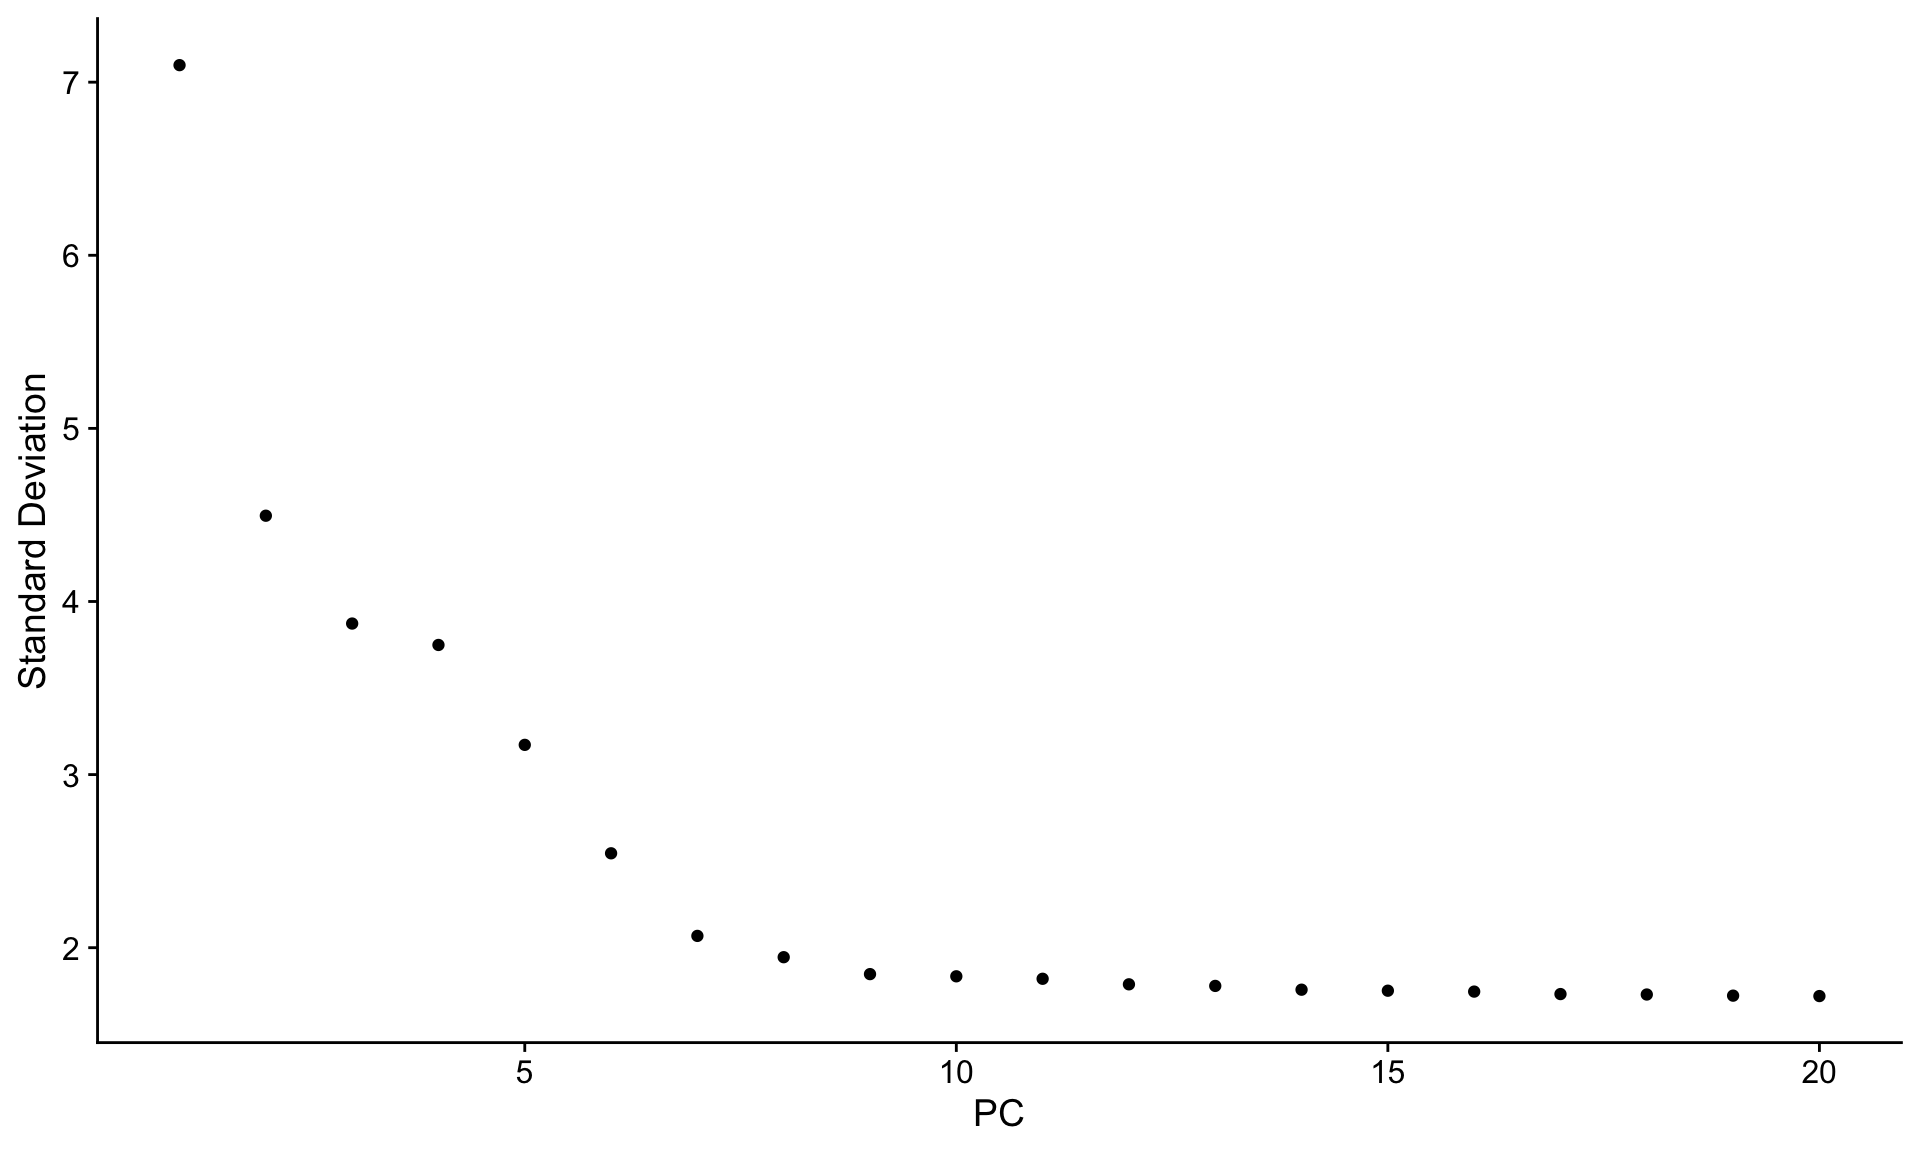
\includegraphics{scRNAseqInR_Doco_files/figure-latex/elbow_plot-1.pdf}

Identifying the true dimensionality of a dataset -- can be challenging/uncertain for the user. We therefore suggest these three approaches to consider. The first is more supervised, exploring PCs to determine relevant sources of heterogeneity, and could be used in conjunction with GSEA for example. The second implements a statistical test based on a random null model, but is time-consuming for large datasets, and may not return a clear PC cutoff. The third is a heuristic that is commonly used, and can be calculated instantly. In this example, all three approaches yielded similar results, but we might have been justified in choosing anything between PC 7-12 as a cutoff.

We chose 10 here, but encourage users to consider the following:

\begin{itemize}
\tightlist
\item
  Dendritic cell and NK aficionados may recognize that genes strongly associated with PCs 12 and 13 define rare immune subsets (i.e.~MZB1 is a marker for plasmacytoid DCs). However, these groups are so rare, they are difficult to distinguish from background noise for a dataset of this size without prior knowledge.
\item
  We encourage users to repeat downstream analyses with a different number of PCs (10, 15, or even 50!). As you will observe, the results often do not differ dramatically.
\item
  We advise users to err on the higher side when choosing this parameter. For example, performing downstream analyses with only 5 PCs does significantly and adversely affect results.
\end{itemize}

\begin{center}\rule{0.5\linewidth}{0.5pt}\end{center}

\hypertarget{run-non-linear-dimensional-reduction-umaptsne}{%
\section{Run non-linear dimensional reduction (UMAP/tSNE)}\label{run-non-linear-dimensional-reduction-umaptsne}}

Seurat offers several non-linear dimensional reduction techniques, such as tSNE and UMAP, to visualize and explore these datasets. The goal of these algorithms is to learn the underlying manifold of the data in order to place similar cells together in low-dimensional space. Cells within the graph-based clusters determined above should co-localize on these dimension reduction plots. As input to the UMAP and tSNE, we suggest using the same PCs as input to the clustering analysis.

\begin{Shaded}
\begin{Highlighting}[]
\CommentTok{\# If you haven\textquotesingle{}t installed UMAP, you can do so via reticulate::py\_install(packages = "umap{-}learn")}
\NormalTok{pbmc }\OtherTok{\textless{}{-}} \FunctionTok{RunUMAP}\NormalTok{(pbmc, }\AttributeTok{dims =} \DecValTok{1}\SpecialCharTok{:}\DecValTok{10}\NormalTok{)}
\CommentTok{\#\textgreater{} Warning: The default method for RunUMAP has changed from calling Python UMAP via reticulate to the R{-}native UWOT using the cosine metric}
\CommentTok{\#\textgreater{} To use Python UMAP via reticulate, set umap.method to \textquotesingle{}umap{-}learn\textquotesingle{} and metric to \textquotesingle{}correlation\textquotesingle{}}
\CommentTok{\#\textgreater{} This message will be shown once per session}
\CommentTok{\#\textgreater{} 10:34:42 UMAP embedding parameters a = 0.9922 b = 1.112}
\CommentTok{\#\textgreater{} 10:34:42 Read 2638 rows and found 10 numeric columns}
\CommentTok{\#\textgreater{} 10:34:42 Using Annoy for neighbor search, n\_neighbors = 30}
\CommentTok{\#\textgreater{} 10:34:42 Building Annoy index with metric = cosine, n\_trees = 50}
\CommentTok{\#\textgreater{} 0\%   10   20   30   40   50   60   70   80   90   100\%}
\CommentTok{\#\textgreater{} [{-}{-}{-}{-}|{-}{-}{-}{-}|{-}{-}{-}{-}|{-}{-}{-}{-}|{-}{-}{-}{-}|{-}{-}{-}{-}|{-}{-}{-}{-}|{-}{-}{-}{-}|{-}{-}{-}{-}|{-}{-}{-}{-}|}
\CommentTok{\#\textgreater{} **************************************************|}
\CommentTok{\#\textgreater{} 10:34:42 Writing NN index file to temp file /var/folders/tp/b078yqdd4ydff9fx87lfttpj\_sc0x3/T//RtmpVlgEIH/file5f4f7df4c007}
\CommentTok{\#\textgreater{} 10:34:42 Searching Annoy index using 1 thread, search\_k = 3000}
\CommentTok{\#\textgreater{} 10:34:43 Annoy recall = 100\%}
\CommentTok{\#\textgreater{} 10:34:43 Commencing smooth kNN distance calibration using 1 thread with target n\_neighbors = 30}
\CommentTok{\#\textgreater{} 10:34:43 Initializing from normalized Laplacian + noise (using irlba)}
\CommentTok{\#\textgreater{} 10:34:43 Commencing optimization for 500 epochs, with 105140 positive edges}
\CommentTok{\#\textgreater{} 10:34:46 Optimization finished}
\end{Highlighting}
\end{Shaded}

\begin{Shaded}
\begin{Highlighting}[]
\CommentTok{\# note that you can set \textasciigrave{}label = TRUE\textasciigrave{} or use the LabelClusters function to help label individual clusters}
\FunctionTok{DimPlot}\NormalTok{(pbmc, }\AttributeTok{reduction =} \StringTok{\textquotesingle{}umap\textquotesingle{}}\NormalTok{)}
\end{Highlighting}
\end{Shaded}

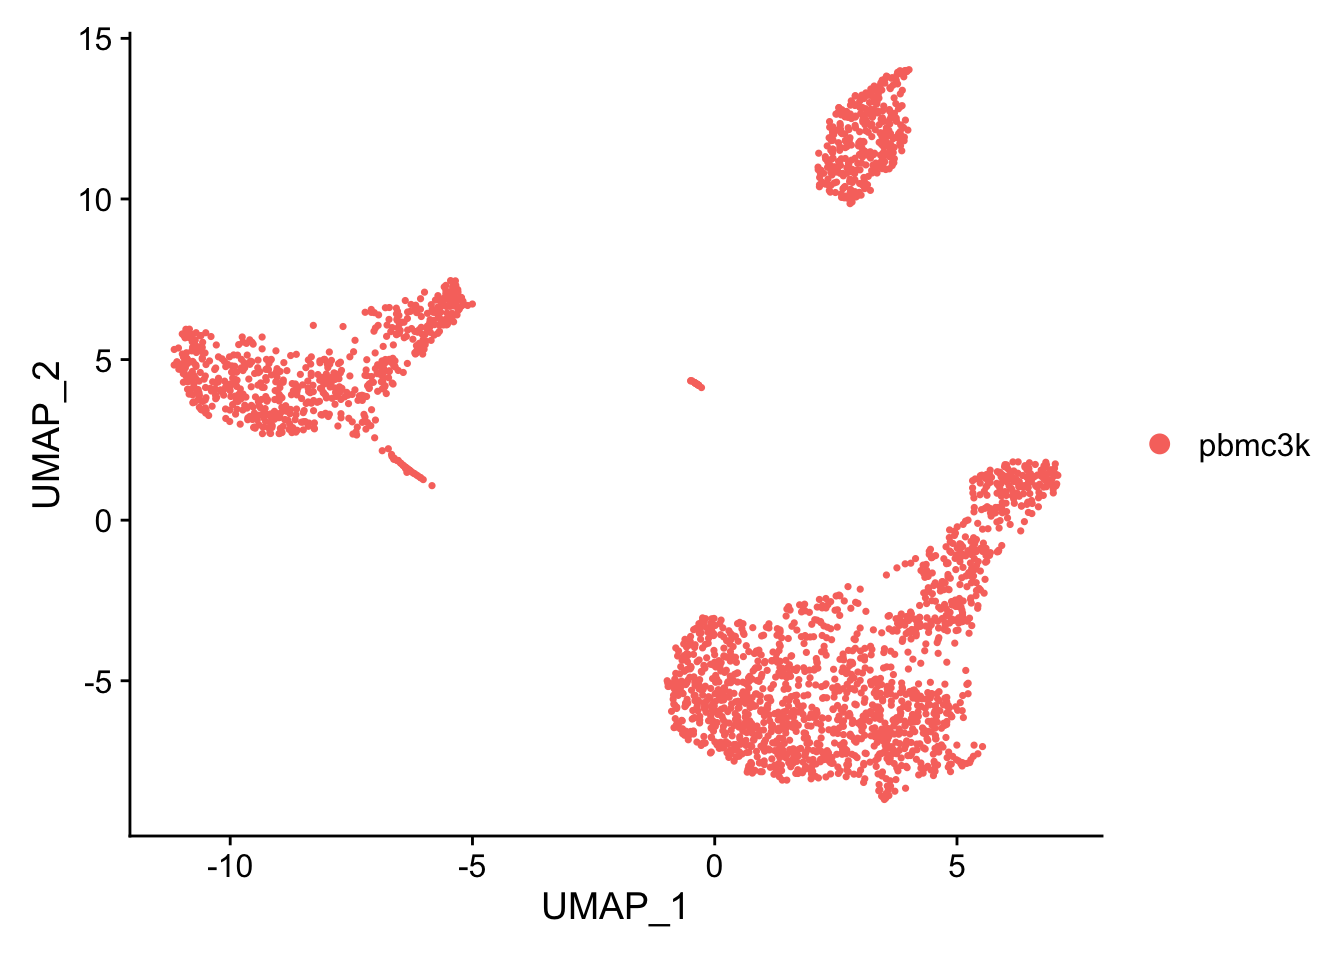
\includegraphics{scRNAseqInR_Doco_files/figure-latex/tsneplot-1.pdf}

You can save the object at this point so that it can easily be loaded back in without having to rerun the computationally intensive steps performed above, or easily shared with collaborators.

\begin{Shaded}
\begin{Highlighting}[]
\FunctionTok{saveRDS}\NormalTok{(pbmc, }\AttributeTok{file =} \StringTok{"pbmc\_tutorial\_saved.rds"}\NormalTok{) }
\end{Highlighting}
\end{Shaded}

\hypertarget{clustering}{%
\chapter{Clustering}\label{clustering}}

\hypertarget{why-do-we-need-to-do-this}{%
\subsubsection*{Why do we need to do this?}\label{why-do-we-need-to-do-this}}
\addcontentsline{toc}{subsubsection}{Why do we need to do this?}

Clustering the cells will allow you to visualise the variability of your data, can help to segregate cells into cell types.

\hypertarget{cluster-cells}{%
\section{Cluster cells}\label{cluster-cells}}

Seurat v3 applies a graph-based clustering approach, building upon initial strategies in (\href{http://www.cell.com/abstract/S0092-8674(15)00549-8}{Macosko \emph{et al}}). Importantly, the \emph{distance metric} which drives the clustering analysis (based on previously identified PCs) remains the same. However, our approach to partitioning the cellular distance matrix into clusters has dramatically improved. Our approach was heavily inspired by recent manuscripts which applied graph-based clustering approaches to scRNA-seq data \href{http://bioinformatics.oxfordjournals.org/content/early/2015/02/10/bioinformatics.btv088.abstract}{{[}SNN-Cliq, Xu and Su, Bioinformatics, 2015{]}} and CyTOF data \href{http://www.ncbi.nlm.nih.gov/pubmed/26095251}{{[}PhenoGraph, Levine \emph{et al}., Cell, 2015{]}}. Briefly, these methods embed cells in a graph structure - for example a K-nearest neighbor (KNN) graph, with edges drawn between cells with similar feature expression patterns, and then attempt to partition this graph into highly interconnected `quasi-cliques' or `communities'.

As in PhenoGraph, we first construct a KNN graph based on the euclidean distance in PCA space, and refine the edge weights between any two cells based on the shared overlap in their local neighborhoods (Jaccard similarity). This step is performed using the \texttt{FindNeighbors()} function, and takes as input the previously defined dimensionality of the dataset (first 10 PCs).

To cluster the cells, we next apply modularity optimization techniques such as the Louvain algorithm (default) or SLM \href{http://dx.doi.org/10.1088/1742-5468/2008/10/P10008}{{[}SLM, Blondel \emph{et al}., Journal of Statistical Mechanics{]}}, to iteratively group cells together, with the goal of optimizing the standard modularity function. The \texttt{FindClusters()} function implements this procedure, and contains a resolution parameter that sets the `granularity' of the downstream clustering, with increased values leading to a greater number of clusters. We find that setting this parameter between 0.4-1.2 typically returns good results for single-cell datasets of around 3K cells. Optimal resolution often increases for larger datasets. The clusters can be found using the \texttt{Idents()} function.

\begin{Shaded}
\begin{Highlighting}[]
\NormalTok{pbmc }\OtherTok{\textless{}{-}} \FunctionTok{FindNeighbors}\NormalTok{(pbmc, }\AttributeTok{dims =} \DecValTok{1}\SpecialCharTok{:}\DecValTok{10}\NormalTok{)}
\CommentTok{\#\textgreater{} Computing nearest neighbor graph}
\CommentTok{\#\textgreater{} Computing SNN}
\NormalTok{pbmc }\OtherTok{\textless{}{-}} \FunctionTok{FindClusters}\NormalTok{(pbmc, }\AttributeTok{resolution =} \FloatTok{0.5}\NormalTok{)}
\CommentTok{\#\textgreater{} Modularity Optimizer version 1.3.0 by Ludo Waltman and Nees Jan van Eck}
\CommentTok{\#\textgreater{} }
\CommentTok{\#\textgreater{} Number of nodes: 2638}
\CommentTok{\#\textgreater{} Number of edges: 95927}
\CommentTok{\#\textgreater{} }
\CommentTok{\#\textgreater{} Running Louvain algorithm...}
\CommentTok{\#\textgreater{} Maximum modularity in 10 random starts: 0.8728}
\CommentTok{\#\textgreater{} Number of communities: 9}
\CommentTok{\#\textgreater{} Elapsed time: 0 seconds}
\CommentTok{\# Look at cluster IDs of the first 5 cells}
\FunctionTok{head}\NormalTok{(}\FunctionTok{Idents}\NormalTok{(pbmc), }\DecValTok{5}\NormalTok{)}
\CommentTok{\#\textgreater{} AAACATACAACCAC{-}1 AAACATTGAGCTAC{-}1 AAACATTGATCAGC{-}1 }
\CommentTok{\#\textgreater{}                2                3                2 }
\CommentTok{\#\textgreater{} AAACCGTGCTTCCG{-}1 AAACCGTGTATGCG{-}1 }
\CommentTok{\#\textgreater{}                1                6 }
\CommentTok{\#\textgreater{} Levels: 0 1 2 3 4 5 6 7 8}
\end{Highlighting}
\end{Shaded}

Check out the clusters.

\begin{Shaded}
\begin{Highlighting}[]
\FunctionTok{DimPlot}\NormalTok{(pbmc)}
\end{Highlighting}
\end{Shaded}

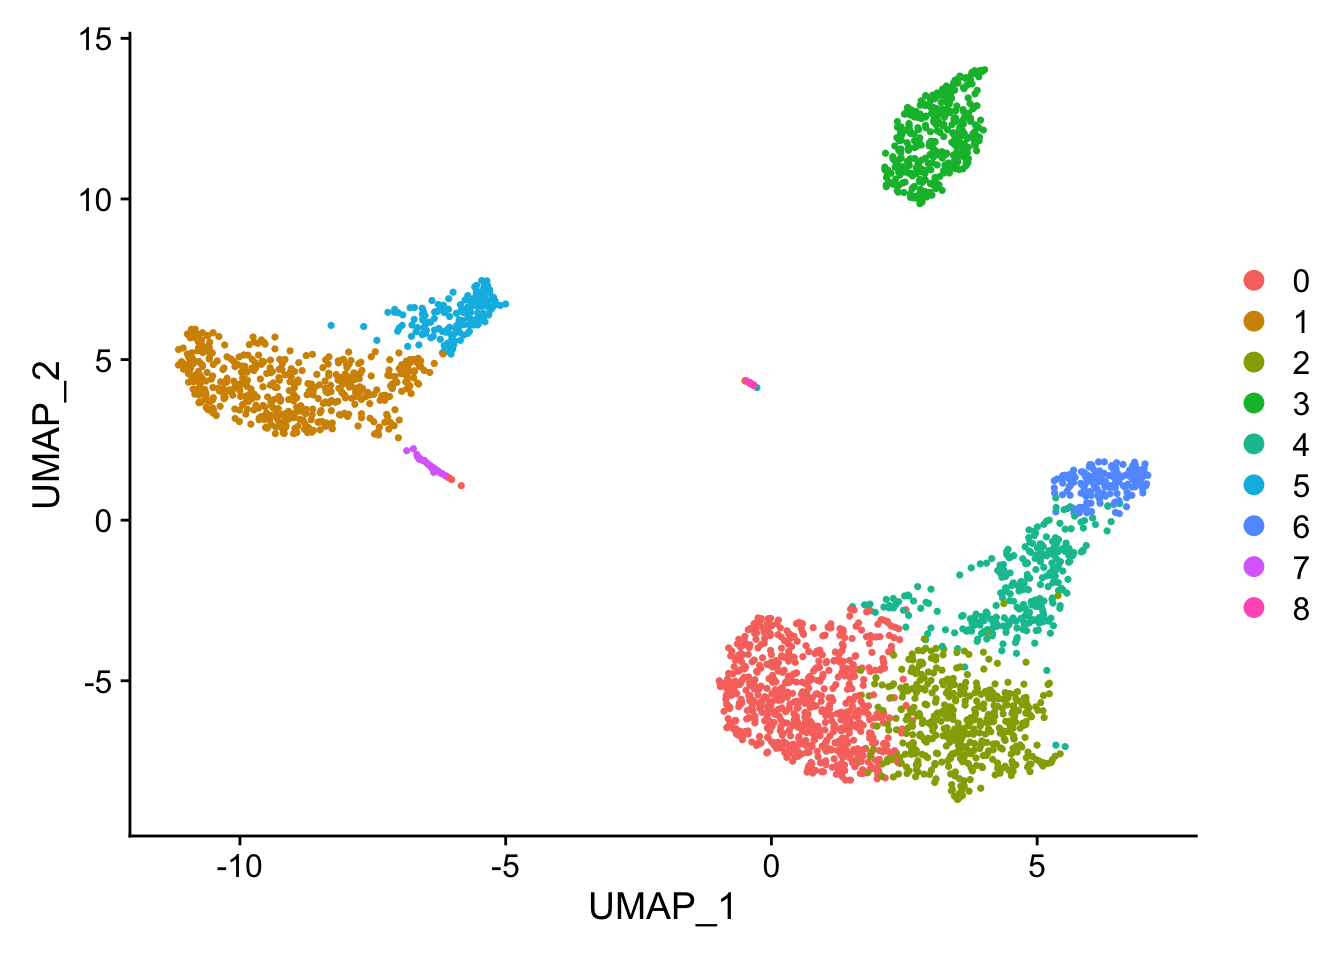
\includegraphics{scRNAseqInR_Doco_files/figure-latex/unnamed-chunk-23-1.pdf}

\begin{Shaded}
\begin{Highlighting}[]
\CommentTok{\# Equivalent to}
\CommentTok{\# DimPlot(pbmc,reduction="umap", group.by="seurat\_clusters")}
\CommentTok{\# DimPlot(pbmc,reduction="umap", group.by="RNA\_snn\_res.0.5")}
\end{Highlighting}
\end{Shaded}

\begin{center}\rule{0.5\linewidth}{0.5pt}\end{center}

\hypertarget{challenge-try-different-cluster-settings}{%
\subsubsection*{Challenge: Try different cluster settings}\label{challenge-try-different-cluster-settings}}
\addcontentsline{toc}{subsubsection}{Challenge: Try different cluster settings}

Run \texttt{FindNeighbours} and \texttt{FindClusters} again, with a different number of dimensions or with a different resolution. Examine the resulting clusters using \texttt{DimPlot}.

To maintain the flow of this tutorial, please put the output of this exploration in a different variable, such as \texttt{pbmc2}!

\hypertarget{choosing-a-cluster-resolution}{%
\section{Choosing a cluster resolution}\label{choosing-a-cluster-resolution}}

Its a good idea to try different resolutions when clustering to identify the varibility of your data.

\begin{Shaded}
\begin{Highlighting}[]
\NormalTok{resolution }\OtherTok{=} \DecValTok{2}
\NormalTok{pbmc }\OtherTok{\textless{}{-}} \FunctionTok{FindClusters}\NormalTok{(}\AttributeTok{object =}\NormalTok{ pbmc, }\AttributeTok{reduction =} \StringTok{"umap"}\NormalTok{, }\AttributeTok{resolution =} \FunctionTok{seq}\NormalTok{(}\FloatTok{0.1}\NormalTok{, resolution, }\FloatTok{0.1}\NormalTok{),}
    \AttributeTok{dims =} \DecValTok{1}\SpecialCharTok{:}\DecValTok{10}\NormalTok{)}
\CommentTok{\#\textgreater{} Warning: The following arguments are not used: reduction,}
\CommentTok{\#\textgreater{} dims}

\CommentTok{\#\textgreater{} Warning: The following arguments are not used: reduction,}
\CommentTok{\#\textgreater{} dims}
\CommentTok{\#\textgreater{} Modularity Optimizer version 1.3.0 by Ludo Waltman and Nees Jan van Eck}
\CommentTok{\#\textgreater{} }
\CommentTok{\#\textgreater{} Number of nodes: 2638}
\CommentTok{\#\textgreater{} Number of edges: 95927}
\CommentTok{\#\textgreater{} }
\CommentTok{\#\textgreater{} Running Louvain algorithm...}
\CommentTok{\#\textgreater{} Maximum modularity in 10 random starts: 0.9623}
\CommentTok{\#\textgreater{} Number of communities: 4}
\CommentTok{\#\textgreater{} Elapsed time: 0 seconds}
\CommentTok{\#\textgreater{} Modularity Optimizer version 1.3.0 by Ludo Waltman and Nees Jan van Eck}
\CommentTok{\#\textgreater{} }
\CommentTok{\#\textgreater{} Number of nodes: 2638}
\CommentTok{\#\textgreater{} Number of edges: 95927}
\CommentTok{\#\textgreater{} }
\CommentTok{\#\textgreater{} Running Louvain algorithm...}
\CommentTok{\#\textgreater{} Maximum modularity in 10 random starts: 0.9346}
\CommentTok{\#\textgreater{} Number of communities: 7}
\CommentTok{\#\textgreater{} Elapsed time: 0 seconds}
\CommentTok{\#\textgreater{} Modularity Optimizer version 1.3.0 by Ludo Waltman and Nees Jan van Eck}
\CommentTok{\#\textgreater{} }
\CommentTok{\#\textgreater{} Number of nodes: 2638}
\CommentTok{\#\textgreater{} Number of edges: 95927}
\CommentTok{\#\textgreater{} }
\CommentTok{\#\textgreater{} Running Louvain algorithm...}
\CommentTok{\#\textgreater{} Maximum modularity in 10 random starts: 0.9091}
\CommentTok{\#\textgreater{} Number of communities: 7}
\CommentTok{\#\textgreater{} Elapsed time: 0 seconds}
\CommentTok{\#\textgreater{} Modularity Optimizer version 1.3.0 by Ludo Waltman and Nees Jan van Eck}
\CommentTok{\#\textgreater{} }
\CommentTok{\#\textgreater{} Number of nodes: 2638}
\CommentTok{\#\textgreater{} Number of edges: 95927}
\CommentTok{\#\textgreater{} }
\CommentTok{\#\textgreater{} Running Louvain algorithm...}
\CommentTok{\#\textgreater{} Maximum modularity in 10 random starts: 0.8890}
\CommentTok{\#\textgreater{} Number of communities: 9}
\CommentTok{\#\textgreater{} Elapsed time: 0 seconds}
\CommentTok{\#\textgreater{} Modularity Optimizer version 1.3.0 by Ludo Waltman and Nees Jan van Eck}
\CommentTok{\#\textgreater{} }
\CommentTok{\#\textgreater{} Number of nodes: 2638}
\CommentTok{\#\textgreater{} Number of edges: 95927}
\CommentTok{\#\textgreater{} }
\CommentTok{\#\textgreater{} Running Louvain algorithm...}
\CommentTok{\#\textgreater{} Maximum modularity in 10 random starts: 0.8728}
\CommentTok{\#\textgreater{} Number of communities: 9}
\CommentTok{\#\textgreater{} Elapsed time: 0 seconds}
\CommentTok{\#\textgreater{} Modularity Optimizer version 1.3.0 by Ludo Waltman and Nees Jan van Eck}
\CommentTok{\#\textgreater{} }
\CommentTok{\#\textgreater{} Number of nodes: 2638}
\CommentTok{\#\textgreater{} Number of edges: 95927}
\CommentTok{\#\textgreater{} }
\CommentTok{\#\textgreater{} Running Louvain algorithm...}
\CommentTok{\#\textgreater{} Maximum modularity in 10 random starts: 0.8564}
\CommentTok{\#\textgreater{} Number of communities: 10}
\CommentTok{\#\textgreater{} Elapsed time: 0 seconds}
\CommentTok{\#\textgreater{} Modularity Optimizer version 1.3.0 by Ludo Waltman and Nees Jan van Eck}
\CommentTok{\#\textgreater{} }
\CommentTok{\#\textgreater{} Number of nodes: 2638}
\CommentTok{\#\textgreater{} Number of edges: 95927}
\CommentTok{\#\textgreater{} }
\CommentTok{\#\textgreater{} Running Louvain algorithm...}
\CommentTok{\#\textgreater{} Maximum modularity in 10 random starts: 0.8411}
\CommentTok{\#\textgreater{} Number of communities: 10}
\CommentTok{\#\textgreater{} Elapsed time: 0 seconds}
\CommentTok{\#\textgreater{} Modularity Optimizer version 1.3.0 by Ludo Waltman and Nees Jan van Eck}
\CommentTok{\#\textgreater{} }
\CommentTok{\#\textgreater{} Number of nodes: 2638}
\CommentTok{\#\textgreater{} Number of edges: 95927}
\CommentTok{\#\textgreater{} }
\CommentTok{\#\textgreater{} Running Louvain algorithm...}
\CommentTok{\#\textgreater{} Maximum modularity in 10 random starts: 0.8281}
\CommentTok{\#\textgreater{} Number of communities: 11}
\CommentTok{\#\textgreater{} Elapsed time: 0 seconds}
\CommentTok{\#\textgreater{} Modularity Optimizer version 1.3.0 by Ludo Waltman and Nees Jan van Eck}
\CommentTok{\#\textgreater{} }
\CommentTok{\#\textgreater{} Number of nodes: 2638}
\CommentTok{\#\textgreater{} Number of edges: 95927}
\CommentTok{\#\textgreater{} }
\CommentTok{\#\textgreater{} Running Louvain algorithm...}
\CommentTok{\#\textgreater{} Maximum modularity in 10 random starts: 0.8159}
\CommentTok{\#\textgreater{} Number of communities: 11}
\CommentTok{\#\textgreater{} Elapsed time: 0 seconds}
\CommentTok{\#\textgreater{} Modularity Optimizer version 1.3.0 by Ludo Waltman and Nees Jan van Eck}
\CommentTok{\#\textgreater{} }
\CommentTok{\#\textgreater{} Number of nodes: 2638}
\CommentTok{\#\textgreater{} Number of edges: 95927}
\CommentTok{\#\textgreater{} }
\CommentTok{\#\textgreater{} Running Louvain algorithm...}
\CommentTok{\#\textgreater{} Maximum modularity in 10 random starts: 0.8036}
\CommentTok{\#\textgreater{} Number of communities: 11}
\CommentTok{\#\textgreater{} Elapsed time: 0 seconds}
\CommentTok{\#\textgreater{} Modularity Optimizer version 1.3.0 by Ludo Waltman and Nees Jan van Eck}
\CommentTok{\#\textgreater{} }
\CommentTok{\#\textgreater{} Number of nodes: 2638}
\CommentTok{\#\textgreater{} Number of edges: 95927}
\CommentTok{\#\textgreater{} }
\CommentTok{\#\textgreater{} Running Louvain algorithm...}
\CommentTok{\#\textgreater{} Maximum modularity in 10 random starts: 0.7918}
\CommentTok{\#\textgreater{} Number of communities: 11}
\CommentTok{\#\textgreater{} Elapsed time: 0 seconds}
\CommentTok{\#\textgreater{} Modularity Optimizer version 1.3.0 by Ludo Waltman and Nees Jan van Eck}
\CommentTok{\#\textgreater{} }
\CommentTok{\#\textgreater{} Number of nodes: 2638}
\CommentTok{\#\textgreater{} Number of edges: 95927}
\CommentTok{\#\textgreater{} }
\CommentTok{\#\textgreater{} Running Louvain algorithm...}
\CommentTok{\#\textgreater{} Maximum modularity in 10 random starts: 0.7798}
\CommentTok{\#\textgreater{} Number of communities: 12}
\CommentTok{\#\textgreater{} Elapsed time: 0 seconds}
\CommentTok{\#\textgreater{} Modularity Optimizer version 1.3.0 by Ludo Waltman and Nees Jan van Eck}
\CommentTok{\#\textgreater{} }
\CommentTok{\#\textgreater{} Number of nodes: 2638}
\CommentTok{\#\textgreater{} Number of edges: 95927}
\CommentTok{\#\textgreater{} }
\CommentTok{\#\textgreater{} Running Louvain algorithm...}
\CommentTok{\#\textgreater{} Maximum modularity in 10 random starts: 0.7678}
\CommentTok{\#\textgreater{} Number of communities: 13}
\CommentTok{\#\textgreater{} Elapsed time: 0 seconds}
\CommentTok{\#\textgreater{} Modularity Optimizer version 1.3.0 by Ludo Waltman and Nees Jan van Eck}
\CommentTok{\#\textgreater{} }
\CommentTok{\#\textgreater{} Number of nodes: 2638}
\CommentTok{\#\textgreater{} Number of edges: 95927}
\CommentTok{\#\textgreater{} }
\CommentTok{\#\textgreater{} Running Louvain algorithm...}
\CommentTok{\#\textgreater{} Maximum modularity in 10 random starts: 0.7575}
\CommentTok{\#\textgreater{} Number of communities: 13}
\CommentTok{\#\textgreater{} Elapsed time: 0 seconds}
\CommentTok{\#\textgreater{} Modularity Optimizer version 1.3.0 by Ludo Waltman and Nees Jan van Eck}
\CommentTok{\#\textgreater{} }
\CommentTok{\#\textgreater{} Number of nodes: 2638}
\CommentTok{\#\textgreater{} Number of edges: 95927}
\CommentTok{\#\textgreater{} }
\CommentTok{\#\textgreater{} Running Louvain algorithm...}
\CommentTok{\#\textgreater{} Maximum modularity in 10 random starts: 0.7473}
\CommentTok{\#\textgreater{} Number of communities: 13}
\CommentTok{\#\textgreater{} Elapsed time: 0 seconds}
\CommentTok{\#\textgreater{} Modularity Optimizer version 1.3.0 by Ludo Waltman and Nees Jan van Eck}
\CommentTok{\#\textgreater{} }
\CommentTok{\#\textgreater{} Number of nodes: 2638}
\CommentTok{\#\textgreater{} Number of edges: 95927}
\CommentTok{\#\textgreater{} }
\CommentTok{\#\textgreater{} Running Louvain algorithm...}
\CommentTok{\#\textgreater{} Maximum modularity in 10 random starts: 0.7370}
\CommentTok{\#\textgreater{} Number of communities: 15}
\CommentTok{\#\textgreater{} Elapsed time: 0 seconds}
\CommentTok{\#\textgreater{} Modularity Optimizer version 1.3.0 by Ludo Waltman and Nees Jan van Eck}
\CommentTok{\#\textgreater{} }
\CommentTok{\#\textgreater{} Number of nodes: 2638}
\CommentTok{\#\textgreater{} Number of edges: 95927}
\CommentTok{\#\textgreater{} }
\CommentTok{\#\textgreater{} Running Louvain algorithm...}
\CommentTok{\#\textgreater{} Maximum modularity in 10 random starts: 0.7280}
\CommentTok{\#\textgreater{} Number of communities: 15}
\CommentTok{\#\textgreater{} Elapsed time: 0 seconds}
\CommentTok{\#\textgreater{} Modularity Optimizer version 1.3.0 by Ludo Waltman and Nees Jan van Eck}
\CommentTok{\#\textgreater{} }
\CommentTok{\#\textgreater{} Number of nodes: 2638}
\CommentTok{\#\textgreater{} Number of edges: 95927}
\CommentTok{\#\textgreater{} }
\CommentTok{\#\textgreater{} Running Louvain algorithm...}
\CommentTok{\#\textgreater{} Maximum modularity in 10 random starts: 0.7185}
\CommentTok{\#\textgreater{} Number of communities: 15}
\CommentTok{\#\textgreater{} Elapsed time: 0 seconds}
\CommentTok{\#\textgreater{} Modularity Optimizer version 1.3.0 by Ludo Waltman and Nees Jan van Eck}
\CommentTok{\#\textgreater{} }
\CommentTok{\#\textgreater{} Number of nodes: 2638}
\CommentTok{\#\textgreater{} Number of edges: 95927}
\CommentTok{\#\textgreater{} }
\CommentTok{\#\textgreater{} Running Louvain algorithm...}
\CommentTok{\#\textgreater{} Maximum modularity in 10 random starts: 0.7093}
\CommentTok{\#\textgreater{} Number of communities: 15}
\CommentTok{\#\textgreater{} Elapsed time: 0 seconds}
\CommentTok{\#\textgreater{} Modularity Optimizer version 1.3.0 by Ludo Waltman and Nees Jan van Eck}
\CommentTok{\#\textgreater{} }
\CommentTok{\#\textgreater{} Number of nodes: 2638}
\CommentTok{\#\textgreater{} Number of edges: 95927}
\CommentTok{\#\textgreater{} }
\CommentTok{\#\textgreater{} Running Louvain algorithm...}
\CommentTok{\#\textgreater{} Maximum modularity in 10 random starts: 0.7002}
\CommentTok{\#\textgreater{} Number of communities: 16}
\CommentTok{\#\textgreater{} Elapsed time: 0 seconds}

\CommentTok{\# the different clustering created}
\FunctionTok{names}\NormalTok{(pbmc}\SpecialCharTok{@}\NormalTok{meta.data)}
\CommentTok{\#\textgreater{}  [1] "orig.ident"      "nCount\_RNA"      "nFeature\_RNA"   }
\CommentTok{\#\textgreater{}  [4] "percent.mt"      "RNA\_snn\_res.0.5" "seurat\_clusters"}
\CommentTok{\#\textgreater{}  [7] "RNA\_snn\_res.0.1" "RNA\_snn\_res.0.2" "RNA\_snn\_res.0.3"}
\CommentTok{\#\textgreater{} [10] "RNA\_snn\_res.0.4" "RNA\_snn\_res.0.6" "RNA\_snn\_res.0.7"}
\CommentTok{\#\textgreater{} [13] "RNA\_snn\_res.0.8" "RNA\_snn\_res.0.9" "RNA\_snn\_res.1"  }
\CommentTok{\#\textgreater{} [16] "RNA\_snn\_res.1.1" "RNA\_snn\_res.1.2" "RNA\_snn\_res.1.3"}
\CommentTok{\#\textgreater{} [19] "RNA\_snn\_res.1.4" "RNA\_snn\_res.1.5" "RNA\_snn\_res.1.6"}
\CommentTok{\#\textgreater{} [22] "RNA\_snn\_res.1.7" "RNA\_snn\_res.1.8" "RNA\_snn\_res.1.9"}
\CommentTok{\#\textgreater{} [25] "RNA\_snn\_res.2"}

\CommentTok{\# Look at cluster IDs of the first 5 cells}
\FunctionTok{head}\NormalTok{(}\FunctionTok{Idents}\NormalTok{(pbmc), }\DecValTok{5}\NormalTok{)}
\CommentTok{\#\textgreater{} AAACATACAACCAC{-}1 AAACATTGAGCTAC{-}1 AAACATTGATCAGC{-}1 }
\CommentTok{\#\textgreater{}                6                1                0 }
\CommentTok{\#\textgreater{} AAACCGTGCTTCCG{-}1 AAACCGTGTATGCG{-}1 }
\CommentTok{\#\textgreater{}                5                8 }
\CommentTok{\#\textgreater{} Levels: 0 1 2 3 4 5 6 7 8 9 10 11 12 13 14 15}
\end{Highlighting}
\end{Shaded}

Plot a clustree to decide how many clusters you have and what resolution capture them.

\begin{Shaded}
\begin{Highlighting}[]
\FunctionTok{library}\NormalTok{(clustree)}
\CommentTok{\#\textgreater{} Loading required package: ggraph}
\FunctionTok{clustree}\NormalTok{(pbmc, }\AttributeTok{prefix =} \StringTok{"RNA\_snn\_res."}\NormalTok{) }\SpecialCharTok{+} \FunctionTok{theme}\NormalTok{(}\AttributeTok{legend.key.size =} \FunctionTok{unit}\NormalTok{(}\FloatTok{0.05}\NormalTok{, }\StringTok{"cm"}\NormalTok{))}
\end{Highlighting}
\end{Shaded}

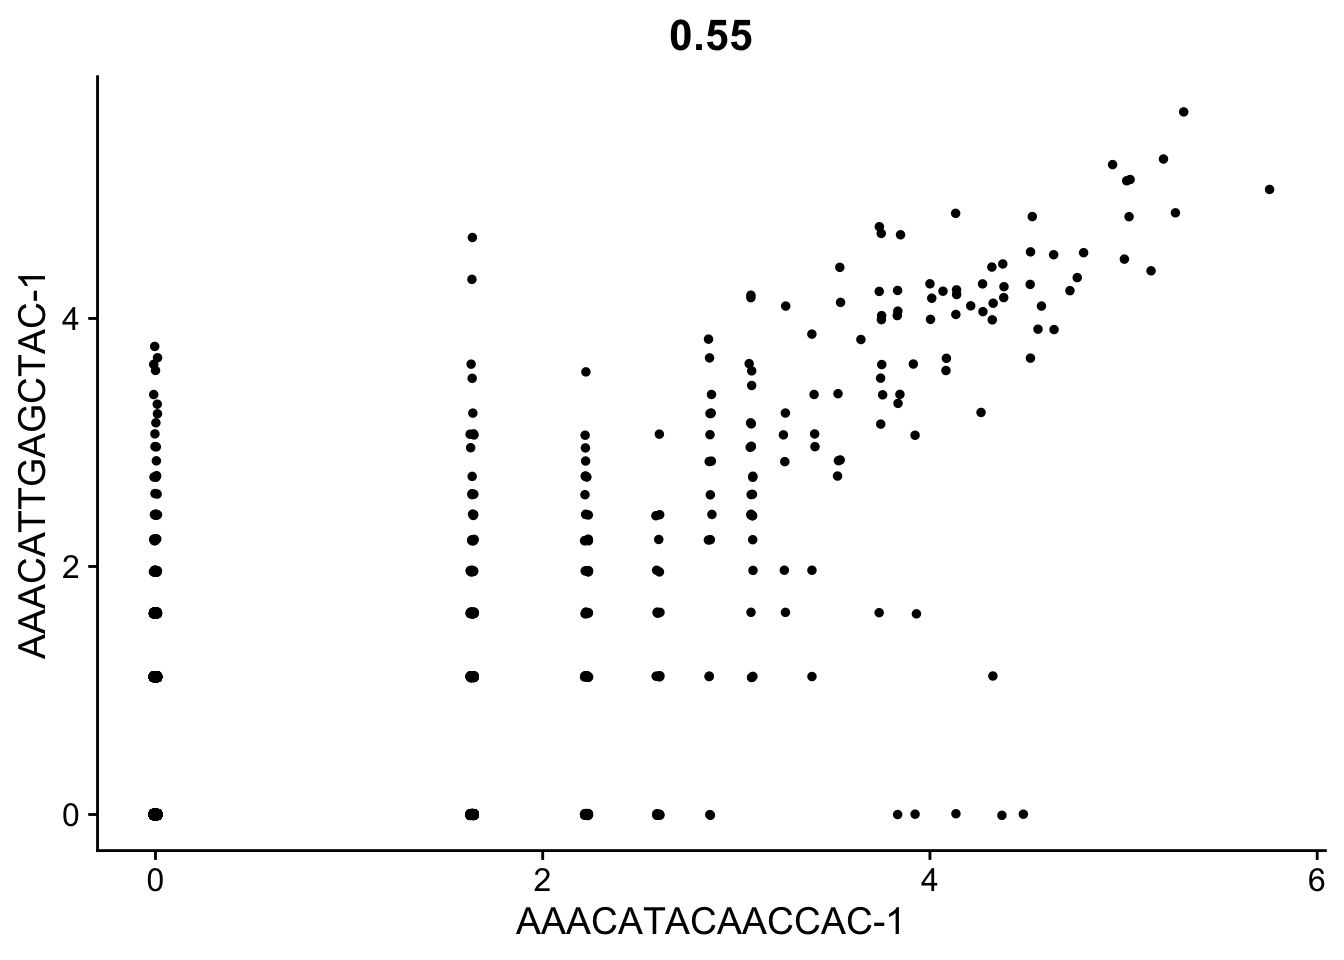
\includegraphics{scRNAseqInR_Doco_files/figure-latex/unnamed-chunk-25-1.pdf}

Name cells with the corresponding cluster name at the resolution you pick. This case we are happy with 0.5.

\begin{Shaded}
\begin{Highlighting}[]
\CommentTok{\# The name of the cluster is prefixed with \textquotesingle{}RNA\_snn\_res\textquotesingle{} and the number of the resolution}
\FunctionTok{Idents}\NormalTok{(pbmc) }\OtherTok{\textless{}{-}}\NormalTok{ pbmc}\SpecialCharTok{$}\NormalTok{RNA\_snn\_res.}\FloatTok{0.5}
\end{Highlighting}
\end{Shaded}

Plot the UMAP with colored clusters with Dimplot

\begin{Shaded}
\begin{Highlighting}[]
\FunctionTok{DimPlot}\NormalTok{(pbmc, }\AttributeTok{label =} \ConstantTok{TRUE}\NormalTok{, }\AttributeTok{repel =} \ConstantTok{TRUE}\NormalTok{, }\AttributeTok{label.box =} \ConstantTok{TRUE}\NormalTok{) }\SpecialCharTok{+} \FunctionTok{NoLegend}\NormalTok{()}
\end{Highlighting}
\end{Shaded}

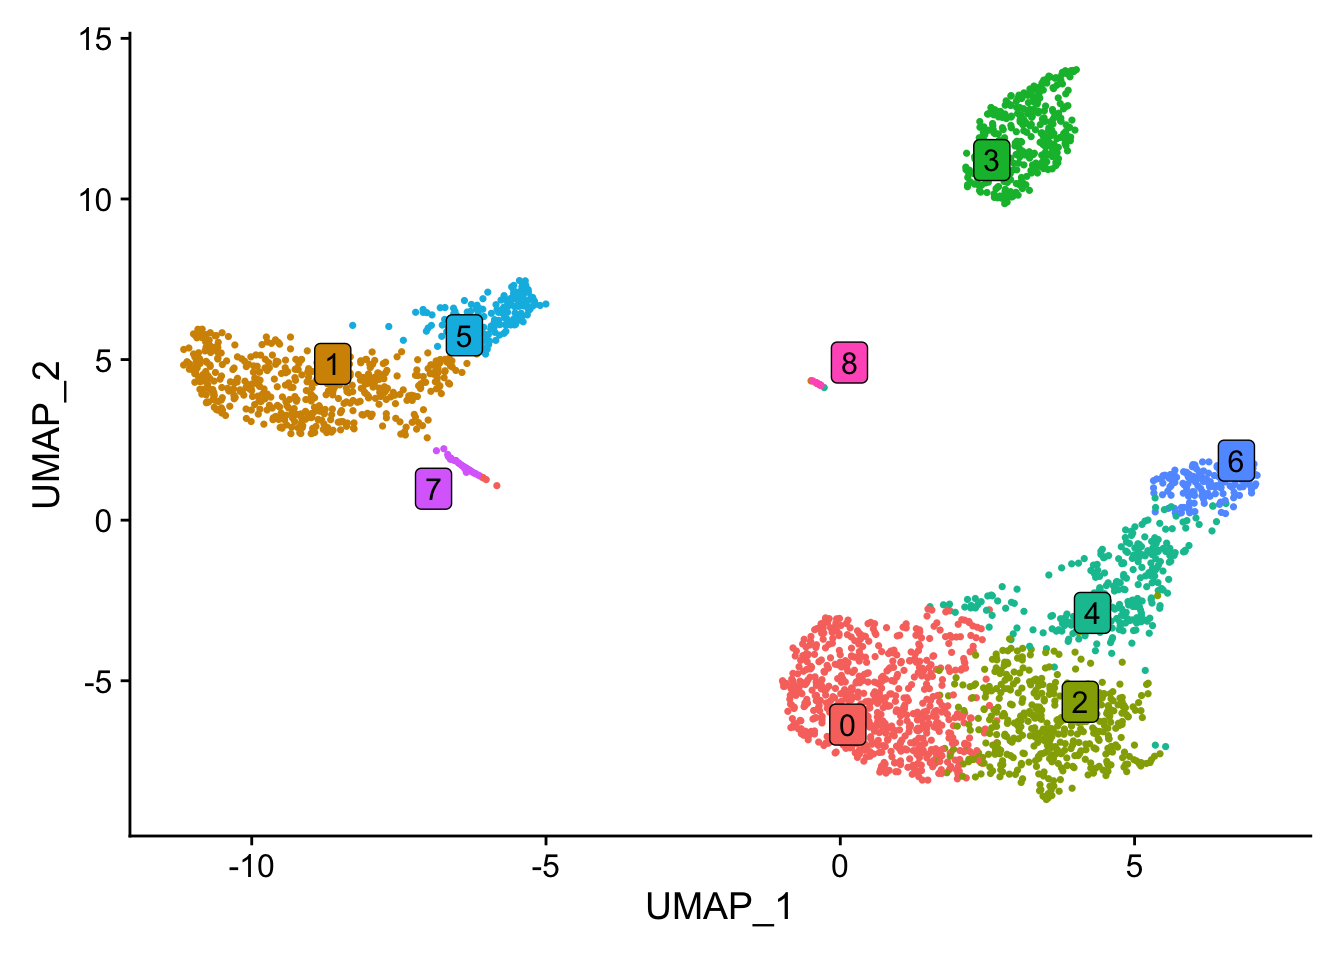
\includegraphics{scRNAseqInR_Doco_files/figure-latex/unnamed-chunk-27-1.pdf}

\hypertarget{clustermarkers}{%
\chapter{Cluster Markers}\label{clustermarkers}}

\hypertarget{why-do-we-need-to-do-this-1}{%
\subsubsection*{Why do we need to do this?}\label{why-do-we-need-to-do-this-1}}
\addcontentsline{toc}{subsubsection}{Why do we need to do this?}

Single cell data helps to segragate cell types. Use markers to identify cell types. warning: In this example the cell types/markers are well known and making this step easy, but in reality this step needs the experts curation.

\begin{center}\rule{0.5\linewidth}{0.5pt}\end{center}

\hypertarget{finding-differentially-expressed-features-cluster-biomarkers}{%
\section{Finding differentially expressed features (cluster biomarkers)}\label{finding-differentially-expressed-features-cluster-biomarkers}}

Seurat can help you find markers that define clusters via differential expression. By default, it identifies positive and negative markers of a single cluster (specified in \texttt{ident.1}), compared to all other cells. \texttt{FindAllMarkers()} automates this process for all clusters, but you can also test groups of clusters vs.~each other, or against all cells.

The \texttt{min.pct} argument requires a feature to be detected at a minimum percentage in either of the two groups of cells, and the thresh.test argument requires a feature to be differentially expressed (on average) by some amount between the two groups. You can set both of these to 0, but with a dramatic increase in time - since this will test a large number of features that are unlikely to be highly discriminatory. As another option to speed up these computations, \texttt{max.cells.per.ident} can be set. This will downsample each identity class to have no more cells than whatever this is set to. While there is generally going to be a loss in power, the speed increases can be significant and the most highly differentially expressed features will likely still rise to the top.

\begin{Shaded}
\begin{Highlighting}[]
\CommentTok{\# find all markers of cluster 2}
\NormalTok{cluster2.markers }\OtherTok{\textless{}{-}} \FunctionTok{FindMarkers}\NormalTok{(pbmc, }\AttributeTok{ident.1 =} \DecValTok{2}\NormalTok{, }\AttributeTok{min.pct =} \FloatTok{0.25}\NormalTok{)}
\FunctionTok{head}\NormalTok{(cluster2.markers, }\AttributeTok{n =} \DecValTok{5}\NormalTok{)}
\CommentTok{\#\textgreater{}             p\_val avg\_log2FC pct.1 pct.2    p\_val\_adj}
\CommentTok{\#\textgreater{} IL32 2.892340e{-}90  1.2013522 0.947 0.465 3.966555e{-}86}
\CommentTok{\#\textgreater{} LTB  1.060121e{-}86  1.2695776 0.981 0.643 1.453850e{-}82}
\CommentTok{\#\textgreater{} CD3D 8.794641e{-}71  0.9389621 0.922 0.432 1.206097e{-}66}
\CommentTok{\#\textgreater{} IL7R 3.516098e{-}68  1.1873213 0.750 0.326 4.821977e{-}64}
\CommentTok{\#\textgreater{} LDHB 1.642480e{-}67  0.8969774 0.954 0.614 2.252497e{-}63}
\CommentTok{\# find all markers distinguishing cluster 5 from clusters 0 and 3}
\NormalTok{cluster5.markers }\OtherTok{\textless{}{-}} \FunctionTok{FindMarkers}\NormalTok{(pbmc, }\AttributeTok{ident.1 =} \DecValTok{5}\NormalTok{, }\AttributeTok{ident.2 =} \FunctionTok{c}\NormalTok{(}\DecValTok{0}\NormalTok{, }\DecValTok{3}\NormalTok{), }\AttributeTok{min.pct =} \FloatTok{0.25}\NormalTok{)}
\FunctionTok{head}\NormalTok{(cluster5.markers, }\AttributeTok{n =} \DecValTok{5}\NormalTok{)}
\CommentTok{\#\textgreater{}                       p\_val avg\_log2FC pct.1 pct.2}
\CommentTok{\#\textgreater{} FCGR3A        8.246578e{-}205   4.261495 0.975 0.040}
\CommentTok{\#\textgreater{} IFITM3        1.677613e{-}195   3.879339 0.975 0.049}
\CommentTok{\#\textgreater{} CFD           2.401156e{-}193   3.405492 0.938 0.038}
\CommentTok{\#\textgreater{} CD68          2.900384e{-}191   3.020484 0.926 0.035}
\CommentTok{\#\textgreater{} RP11{-}290F20.3 2.513244e{-}186   2.720057 0.840 0.017}
\CommentTok{\#\textgreater{}                   p\_val\_adj}
\CommentTok{\#\textgreater{} FCGR3A        1.130936e{-}200}
\CommentTok{\#\textgreater{} IFITM3        2.300678e{-}191}
\CommentTok{\#\textgreater{} CFD           3.292945e{-}189}
\CommentTok{\#\textgreater{} CD68          3.977587e{-}187}
\CommentTok{\#\textgreater{} RP11{-}290F20.3 3.446663e{-}182}
\CommentTok{\# find markers for every cluster compared to all remaining cells, report only the positive ones}
\NormalTok{pbmc.markers }\OtherTok{\textless{}{-}} \FunctionTok{FindAllMarkers}\NormalTok{(pbmc, }\AttributeTok{only.pos =} \ConstantTok{TRUE}\NormalTok{, }\AttributeTok{min.pct =} \FloatTok{0.25}\NormalTok{, }\AttributeTok{logfc.threshold =} \FloatTok{0.25}\NormalTok{)}
\CommentTok{\#\textgreater{} Calculating cluster 0}
\CommentTok{\#\textgreater{} Calculating cluster 1}
\CommentTok{\#\textgreater{} Calculating cluster 2}
\CommentTok{\#\textgreater{} Calculating cluster 3}
\CommentTok{\#\textgreater{} Calculating cluster 4}
\CommentTok{\#\textgreater{} Calculating cluster 5}
\CommentTok{\#\textgreater{} Calculating cluster 6}
\CommentTok{\#\textgreater{} Calculating cluster 7}
\CommentTok{\#\textgreater{} Calculating cluster 8}
\NormalTok{pbmc.markers }\SpecialCharTok{\%\textgreater{}\%} \FunctionTok{group\_by}\NormalTok{(cluster) }\SpecialCharTok{\%\textgreater{}\%} \FunctionTok{slice\_max}\NormalTok{(}\AttributeTok{n =} \DecValTok{2}\NormalTok{, }\AttributeTok{order\_by =}\NormalTok{ avg\_log2FC)}
\CommentTok{\#\textgreater{} \# A tibble: 18 x 7}
\CommentTok{\#\textgreater{} \# Groups:   cluster [9]}
\CommentTok{\#\textgreater{}        p\_val avg\_log2FC pct.1 pct.2 p\_val\_adj cluster gene  }
\CommentTok{\#\textgreater{}        \textless{}dbl\textgreater{}      \textless{}dbl\textgreater{} \textless{}dbl\textgreater{} \textless{}dbl\textgreater{}     \textless{}dbl\textgreater{} \textless{}fct\textgreater{}   \textless{}chr\textgreater{} }
\CommentTok{\#\textgreater{}  1 9.57e{-} 88       1.36 0.447 0.108 1.31e{-} 83 0       CCR7  }
\CommentTok{\#\textgreater{}  2 3.75e{-}112       1.09 0.912 0.592 5.14e{-}108 0       LDHB  }
\CommentTok{\#\textgreater{}  3 0               5.57 0.996 0.215 0         1       S100A9}
\CommentTok{\#\textgreater{}  4 0               5.48 0.975 0.121 0         1       S100A8}
\CommentTok{\#\textgreater{}  5 1.06e{-} 86       1.27 0.981 0.643 1.45e{-} 82 2       LTB   }
\CommentTok{\#\textgreater{}  6 2.97e{-} 58       1.23 0.42  0.111 4.07e{-} 54 2       AQP3  }
\CommentTok{\#\textgreater{}  7 0               4.31 0.936 0.041 0         3       CD79A }
\CommentTok{\#\textgreater{}  8 9.48e{-}271       3.59 0.622 0.022 1.30e{-}266 3       TCL1A }
\CommentTok{\#\textgreater{}  9 5.61e{-}202       3.10 0.983 0.234 7.70e{-}198 4       CCL5  }
\CommentTok{\#\textgreater{} 10 7.25e{-}165       3.00 0.577 0.055 9.95e{-}161 4       GZMK  }
\CommentTok{\#\textgreater{} 11 3.51e{-}184       3.31 0.975 0.134 4.82e{-}180 5       FCGR3A}
\CommentTok{\#\textgreater{} 12 2.03e{-}125       3.09 1     0.315 2.78e{-}121 5       LST1  }
\CommentTok{\#\textgreater{} 13 3.13e{-}191       5.32 0.961 0.131 4.30e{-}187 6       GNLY  }
\CommentTok{\#\textgreater{} 14 7.95e{-}269       4.83 0.961 0.068 1.09e{-}264 6       GZMB  }
\CommentTok{\#\textgreater{} 15 1.48e{-}220       3.87 0.812 0.011 2.03e{-}216 7       FCER1A}
\CommentTok{\#\textgreater{} 16 1.67e{-} 21       2.87 1     0.513 2.28e{-} 17 7       HLA{-}D\textasciitilde{}}
\CommentTok{\#\textgreater{} 17 1.92e{-}102       8.59 1     0.024 2.63e{-} 98 8       PPBP  }
\CommentTok{\#\textgreater{} 18 9.25e{-}186       7.29 1     0.011 1.27e{-}181 8       PF4}
\end{Highlighting}
\end{Shaded}

Seurat has several tests for differential expression which can be set with the test.use parameter (see our \href{de_vignette.html}{DE vignette} for details). For example, the ROC test returns the `classification power' \texttt{abs(AUC-0.5)*2} for any individual marker, ranging from 0 = random to 1 = perfect.

\begin{Shaded}
\begin{Highlighting}[]
\NormalTok{cluster0.markers }\OtherTok{\textless{}{-}} \FunctionTok{FindMarkers}\NormalTok{(pbmc, }\AttributeTok{ident.1 =} \DecValTok{0}\NormalTok{, }\AttributeTok{logfc.threshold =} \FloatTok{0.25}\NormalTok{, }\AttributeTok{test.use =} \StringTok{"roc"}\NormalTok{, }\AttributeTok{only.pos =} \ConstantTok{TRUE}\NormalTok{)}
\end{Highlighting}
\end{Shaded}

We include several tools for visualizing marker expression. \texttt{VlnPlot()} (shows expression probability distributions across clusters), and \texttt{FeaturePlot()} (visualizes feature expression on a tSNE or PCA plot) are our most commonly used visualizations. We also suggest exploring \texttt{RidgePlot()}, \texttt{CellScatter()}, and \texttt{DotPlot()} as additional methods to view your dataset.

\begin{Shaded}
\begin{Highlighting}[]
\FunctionTok{VlnPlot}\NormalTok{(pbmc, }\AttributeTok{features =} \FunctionTok{c}\NormalTok{(}\StringTok{"MS4A1"}\NormalTok{, }\StringTok{"CD79A"}\NormalTok{))}
\end{Highlighting}
\end{Shaded}

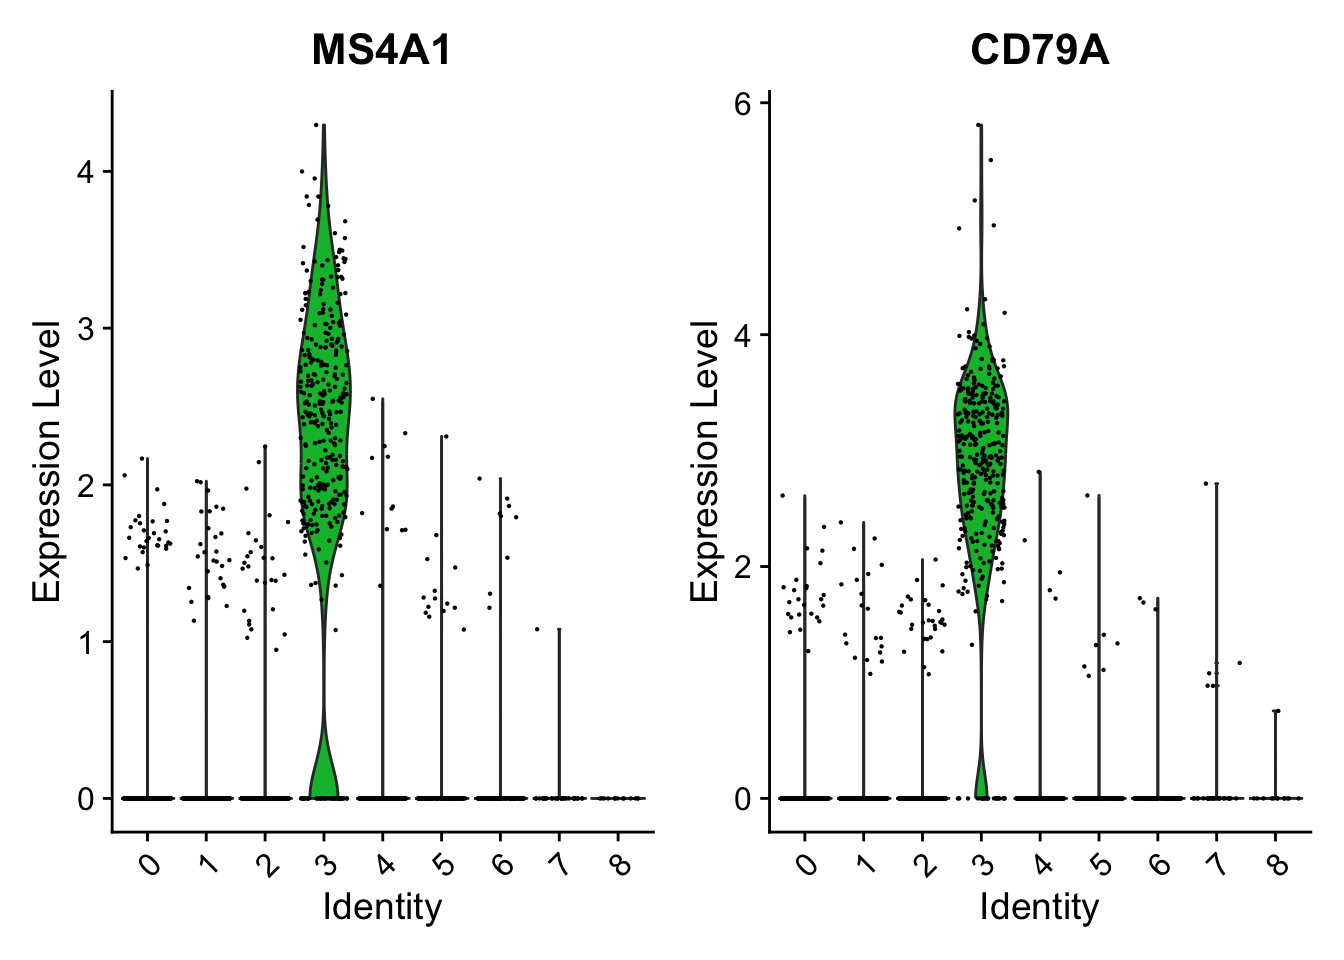
\includegraphics{scRNAseqInR_Doco_files/figure-latex/unnamed-chunk-29-1.pdf}

\begin{Shaded}
\begin{Highlighting}[]
\CommentTok{\# you can plot raw counts as well}
\FunctionTok{VlnPlot}\NormalTok{(pbmc, }\AttributeTok{features =} \FunctionTok{c}\NormalTok{(}\StringTok{"NKG7"}\NormalTok{, }\StringTok{"PF4"}\NormalTok{), }\AttributeTok{slot =} \StringTok{\textquotesingle{}counts\textquotesingle{}}\NormalTok{, }\AttributeTok{log =} \ConstantTok{TRUE}\NormalTok{)}
\end{Highlighting}
\end{Shaded}

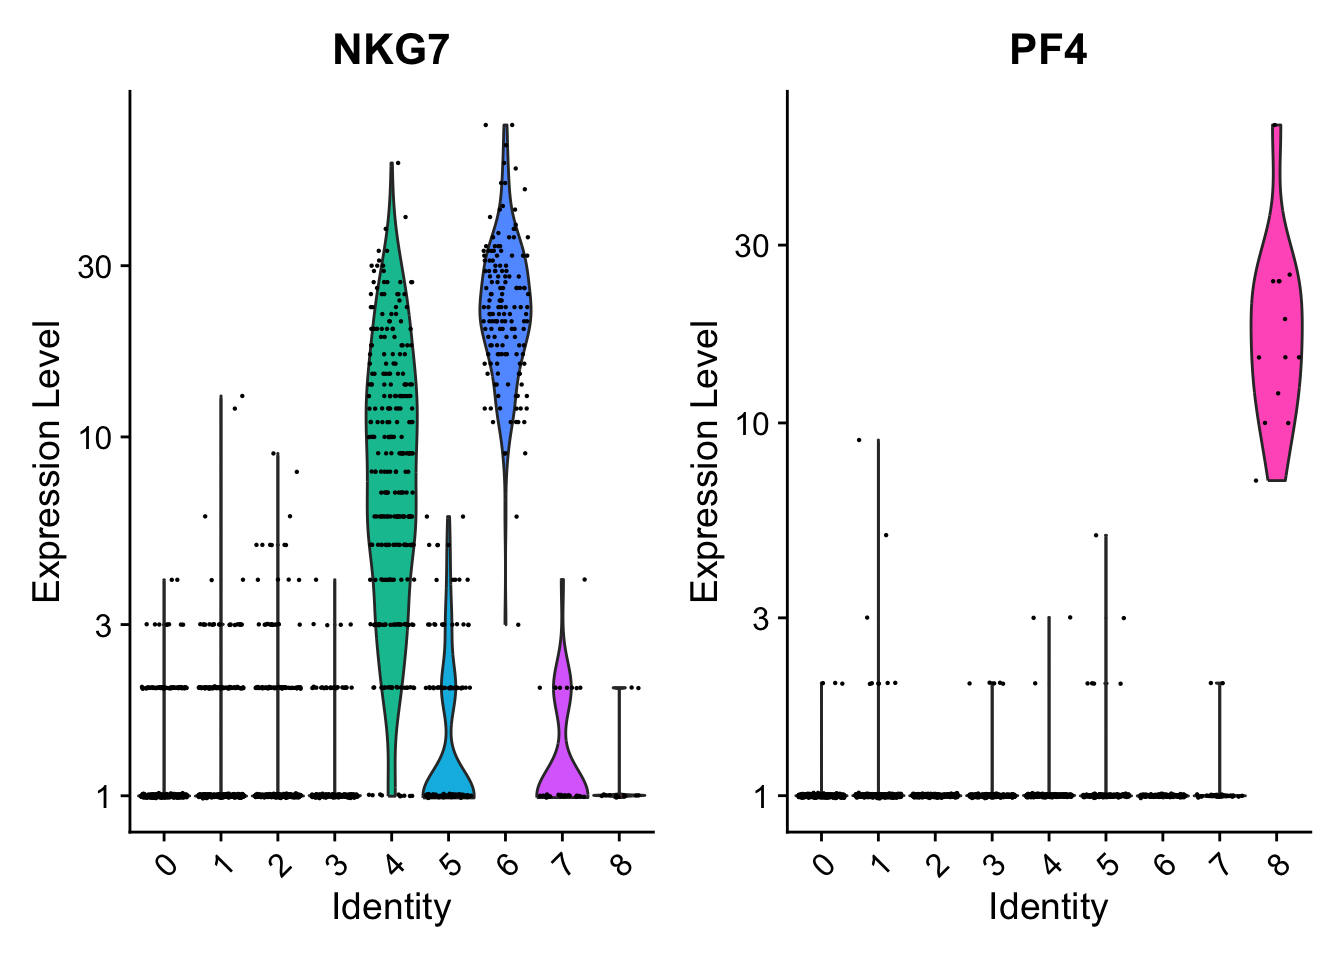
\includegraphics{scRNAseqInR_Doco_files/figure-latex/unnamed-chunk-29-2.pdf}

\begin{Shaded}
\begin{Highlighting}[]
\FunctionTok{FeaturePlot}\NormalTok{(pbmc, }\AttributeTok{features =} \FunctionTok{c}\NormalTok{(}\StringTok{"MS4A1"}\NormalTok{, }\StringTok{"GNLY"}\NormalTok{, }\StringTok{"CD3E"}\NormalTok{, }\StringTok{"CD14"}\NormalTok{, }\StringTok{"FCER1A"}\NormalTok{, }\StringTok{"FCGR3A"}\NormalTok{, }\StringTok{"LYZ"}\NormalTok{, }\StringTok{"PPBP"}\NormalTok{, }\StringTok{"CD8A"}\NormalTok{))}
\end{Highlighting}
\end{Shaded}

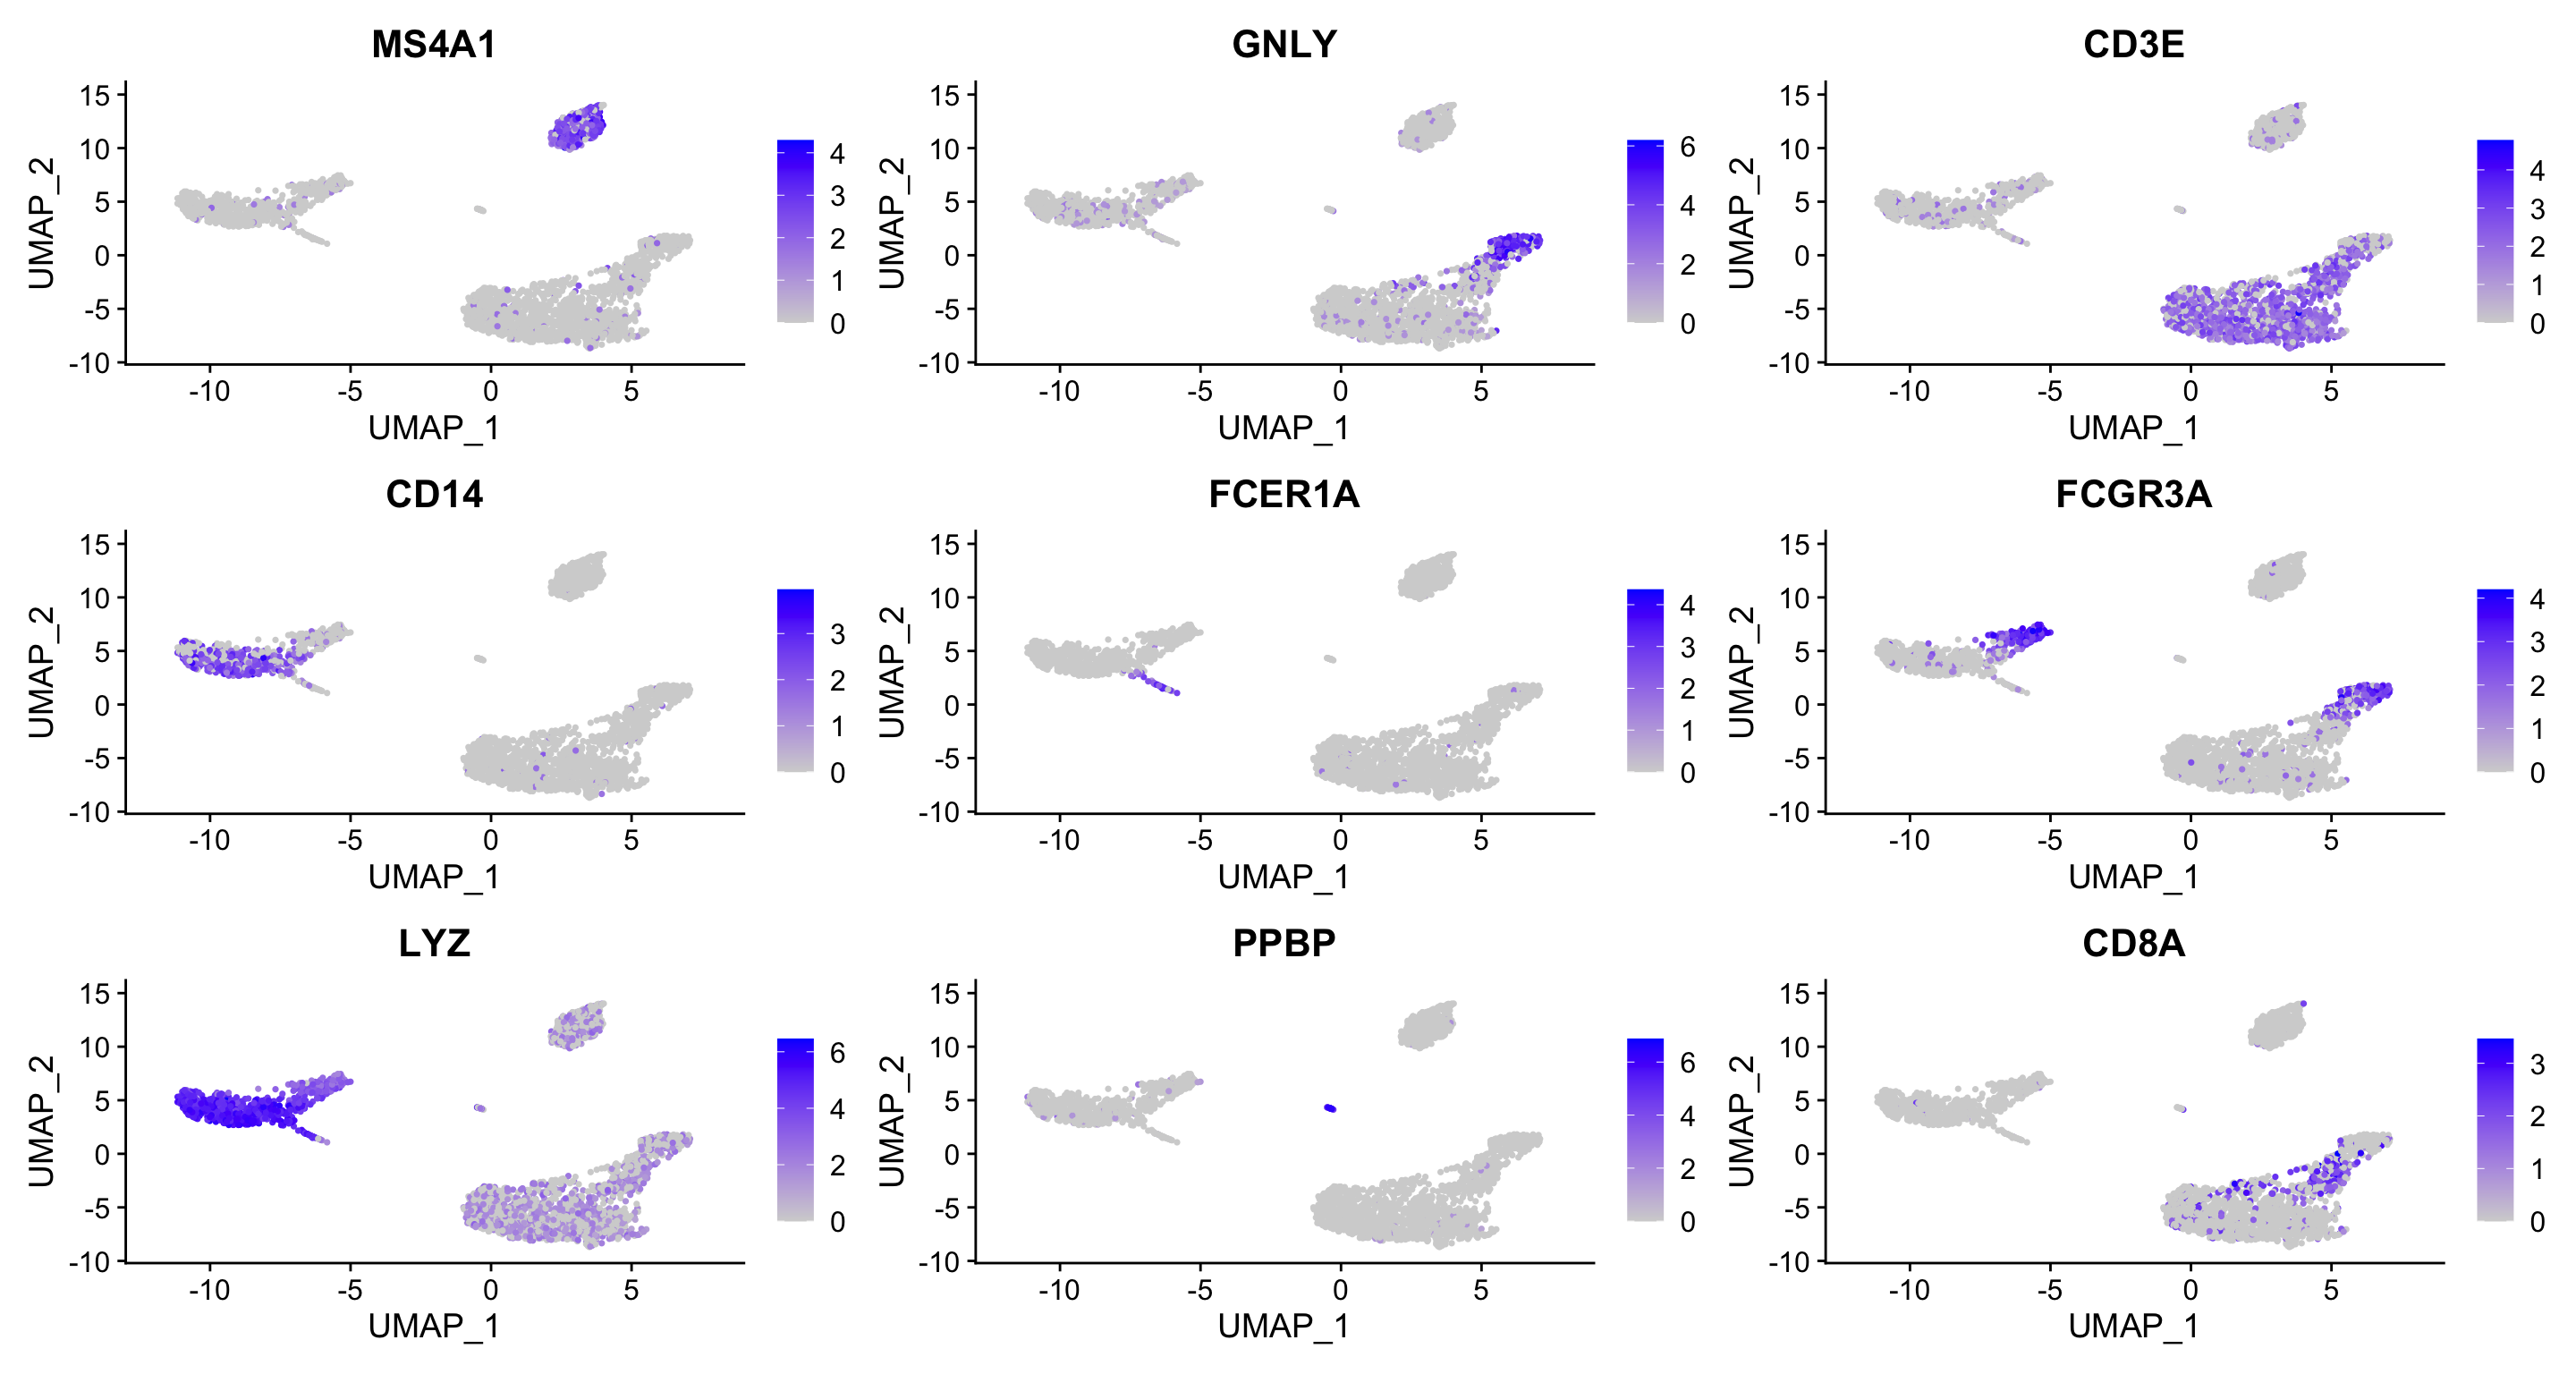
\includegraphics{scRNAseqInR_Doco_files/figure-latex/markerplots-1.pdf}

\textbf{Other useful plots}

These are ridgeplots, cell scatter plots and dotplots. Replace \texttt{FeaturePlot} with the other functions.

\begin{Shaded}
\begin{Highlighting}[]
\FunctionTok{RidgePlot}\NormalTok{(pbmc, }\AttributeTok{features =} \FunctionTok{c}\NormalTok{(}\StringTok{"MS4A1"}\NormalTok{, }\StringTok{"GNLY"}\NormalTok{, }\StringTok{"CD3E"}\NormalTok{, }\StringTok{"CD14"}\NormalTok{, }\StringTok{"FCER1A"}\NormalTok{, }\StringTok{"FCGR3A"}\NormalTok{, }\StringTok{"LYZ"}\NormalTok{, }\StringTok{"PPBP"}\NormalTok{, }\StringTok{"CD8A"}\NormalTok{))}
\CommentTok{\#\textgreater{} Picking joint bandwidth of 0.0236}
\CommentTok{\#\textgreater{} Picking joint bandwidth of 0.0859}
\CommentTok{\#\textgreater{} Picking joint bandwidth of 0.126}
\CommentTok{\#\textgreater{} Picking joint bandwidth of 0.0337}
\CommentTok{\#\textgreater{} Picking joint bandwidth of 0.0659}
\CommentTok{\#\textgreater{} Picking joint bandwidth of 0.0582}
\CommentTok{\#\textgreater{} Picking joint bandwidth of 0.309}
\CommentTok{\#\textgreater{} Picking joint bandwidth of 0.0156}
\CommentTok{\#\textgreater{} Picking joint bandwidth of 0.0366}
\end{Highlighting}
\end{Shaded}

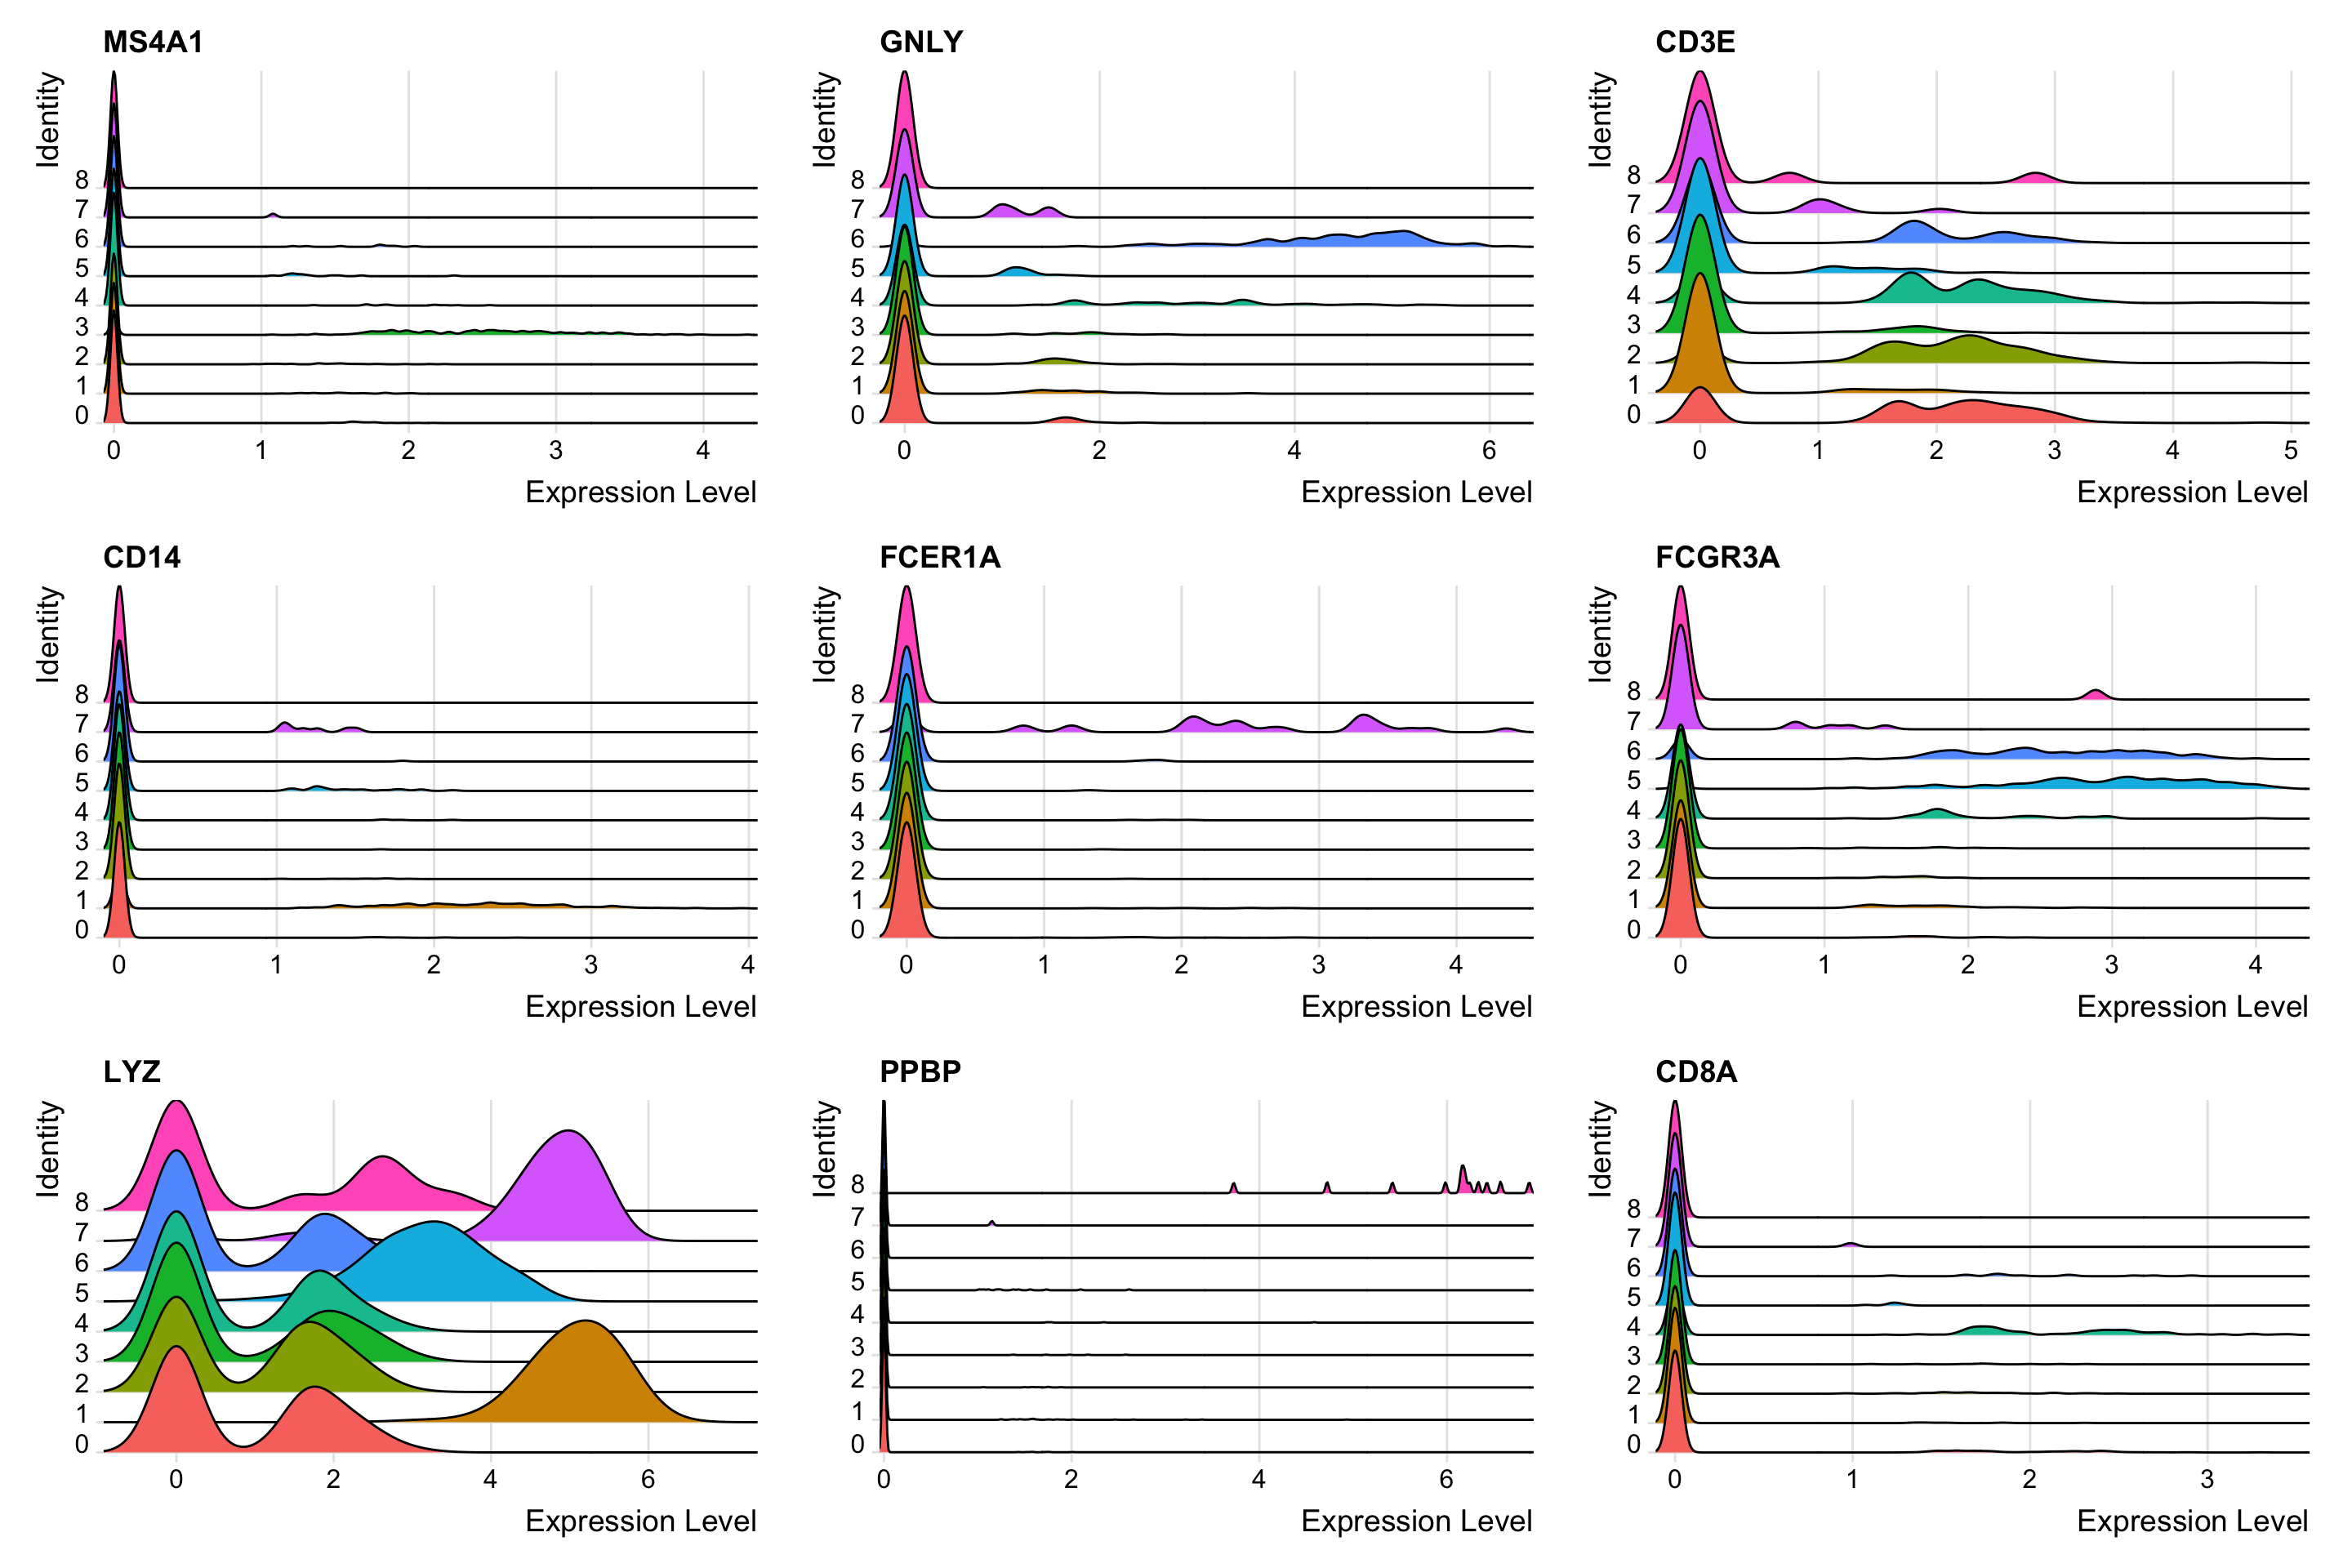
\includegraphics{scRNAseqInR_Doco_files/figure-latex/ridgeplots-1.pdf}
For CellScatter plots, will need the cell id of the cells you want to look at. You can get this from the cell metadata (\texttt{pbmc@meta.data}).

\begin{Shaded}
\begin{Highlighting}[]
\FunctionTok{head}\NormalTok{( pbmc}\SpecialCharTok{@}\NormalTok{meta.data )}
\CommentTok{\#\textgreater{}                  orig.ident nCount\_RNA nFeature\_RNA}
\CommentTok{\#\textgreater{} AAACATACAACCAC{-}1     pbmc3k       2419          779}
\CommentTok{\#\textgreater{} AAACATTGAGCTAC{-}1     pbmc3k       4903         1352}
\CommentTok{\#\textgreater{} AAACATTGATCAGC{-}1     pbmc3k       3147         1129}
\CommentTok{\#\textgreater{} AAACCGTGCTTCCG{-}1     pbmc3k       2639          960}
\CommentTok{\#\textgreater{} AAACCGTGTATGCG{-}1     pbmc3k        980          521}
\CommentTok{\#\textgreater{} AAACGCACTGGTAC{-}1     pbmc3k       2163          781}
\CommentTok{\#\textgreater{}                  percent.mt RNA\_snn\_res.0.5 seurat\_clusters}
\CommentTok{\#\textgreater{} AAACATACAACCAC{-}1  3.0177759               2               6}
\CommentTok{\#\textgreater{} AAACATTGAGCTAC{-}1  3.7935958               3               1}
\CommentTok{\#\textgreater{} AAACATTGATCAGC{-}1  0.8897363               2               0}
\CommentTok{\#\textgreater{} AAACCGTGCTTCCG{-}1  1.7430845               1               5}
\CommentTok{\#\textgreater{} AAACCGTGTATGCG{-}1  1.2244898               6               8}
\CommentTok{\#\textgreater{} AAACGCACTGGTAC{-}1  1.6643551               2               0}
\CommentTok{\#\textgreater{}                  RNA\_snn\_res.0.1 RNA\_snn\_res.0.2}
\CommentTok{\#\textgreater{} AAACATACAACCAC{-}1               0               0}
\CommentTok{\#\textgreater{} AAACATTGAGCTAC{-}1               3               3}
\CommentTok{\#\textgreater{} AAACATTGATCAGC{-}1               0               0}
\CommentTok{\#\textgreater{} AAACCGTGCTTCCG{-}1               1               1}
\CommentTok{\#\textgreater{} AAACCGTGTATGCG{-}1               2               2}
\CommentTok{\#\textgreater{} AAACGCACTGGTAC{-}1               0               0}
\CommentTok{\#\textgreater{}                  RNA\_snn\_res.0.3 RNA\_snn\_res.0.4}
\CommentTok{\#\textgreater{} AAACATACAACCAC{-}1               0               2}
\CommentTok{\#\textgreater{} AAACATTGAGCTAC{-}1               3               3}
\CommentTok{\#\textgreater{} AAACATTGATCAGC{-}1               0               2}
\CommentTok{\#\textgreater{} AAACCGTGCTTCCG{-}1               1               1}
\CommentTok{\#\textgreater{} AAACCGTGTATGCG{-}1               2               6}
\CommentTok{\#\textgreater{} AAACGCACTGGTAC{-}1               0               2}
\CommentTok{\#\textgreater{}                  RNA\_snn\_res.0.6 RNA\_snn\_res.0.7}
\CommentTok{\#\textgreater{} AAACATACAACCAC{-}1               1               1}
\CommentTok{\#\textgreater{} AAACATTGAGCTAC{-}1               3               3}
\CommentTok{\#\textgreater{} AAACATTGATCAGC{-}1               1               1}
\CommentTok{\#\textgreater{} AAACCGTGCTTCCG{-}1               2               2}
\CommentTok{\#\textgreater{} AAACCGTGTATGCG{-}1               6               6}
\CommentTok{\#\textgreater{} AAACGCACTGGTAC{-}1               1               1}
\CommentTok{\#\textgreater{}                  RNA\_snn\_res.0.8 RNA\_snn\_res.0.9}
\CommentTok{\#\textgreater{} AAACATACAACCAC{-}1               6               1}
\CommentTok{\#\textgreater{} AAACATTGAGCTAC{-}1               2               2}
\CommentTok{\#\textgreater{} AAACATTGATCAGC{-}1               1               1}
\CommentTok{\#\textgreater{} AAACCGTGCTTCCG{-}1               4               4}
\CommentTok{\#\textgreater{} AAACCGTGTATGCG{-}1               8               7}
\CommentTok{\#\textgreater{} AAACGCACTGGTAC{-}1               1               1}
\CommentTok{\#\textgreater{}                  RNA\_snn\_res.1 RNA\_snn\_res.1.1}
\CommentTok{\#\textgreater{} AAACATACAACCAC{-}1             6               6}
\CommentTok{\#\textgreater{} AAACATTGAGCTAC{-}1             2               2}
\CommentTok{\#\textgreater{} AAACATTGATCAGC{-}1             1               1}
\CommentTok{\#\textgreater{} AAACCGTGCTTCCG{-}1             4               4}
\CommentTok{\#\textgreater{} AAACCGTGTATGCG{-}1             8               8}
\CommentTok{\#\textgreater{} AAACGCACTGGTAC{-}1             1               1}
\CommentTok{\#\textgreater{}                  RNA\_snn\_res.1.2 RNA\_snn\_res.1.3}
\CommentTok{\#\textgreater{} AAACATACAACCAC{-}1               6               8}
\CommentTok{\#\textgreater{} AAACATTGAGCTAC{-}1               2               2}
\CommentTok{\#\textgreater{} AAACATTGATCAGC{-}1               1               0}
\CommentTok{\#\textgreater{} AAACCGTGCTTCCG{-}1               4               5}
\CommentTok{\#\textgreater{} AAACCGTGTATGCG{-}1               8               9}
\CommentTok{\#\textgreater{} AAACGCACTGGTAC{-}1               1               0}
\CommentTok{\#\textgreater{}                  RNA\_snn\_res.1.4 RNA\_snn\_res.1.5}
\CommentTok{\#\textgreater{} AAACATACAACCAC{-}1               8               9}
\CommentTok{\#\textgreater{} AAACATTGAGCTAC{-}1               2               2}
\CommentTok{\#\textgreater{} AAACATTGATCAGC{-}1               0               1}
\CommentTok{\#\textgreater{} AAACCGTGCTTCCG{-}1               5               4}
\CommentTok{\#\textgreater{} AAACCGTGTATGCG{-}1               9               8}
\CommentTok{\#\textgreater{} AAACGCACTGGTAC{-}1               0               1}
\CommentTok{\#\textgreater{}                  RNA\_snn\_res.1.6 RNA\_snn\_res.1.7}
\CommentTok{\#\textgreater{} AAACATACAACCAC{-}1               8               8}
\CommentTok{\#\textgreater{} AAACATTGAGCTAC{-}1               1               1}
\CommentTok{\#\textgreater{} AAACATTGATCAGC{-}1               0               0}
\CommentTok{\#\textgreater{} AAACCGTGCTTCCG{-}1               3               3}
\CommentTok{\#\textgreater{} AAACCGTGTATGCG{-}1               7               7}
\CommentTok{\#\textgreater{} AAACGCACTGGTAC{-}1               0               0}
\CommentTok{\#\textgreater{}                  RNA\_snn\_res.1.8 RNA\_snn\_res.1.9}
\CommentTok{\#\textgreater{} AAACATACAACCAC{-}1               7               6}
\CommentTok{\#\textgreater{} AAACATTGAGCTAC{-}1               1               1}
\CommentTok{\#\textgreater{} AAACATTGATCAGC{-}1               0               0}
\CommentTok{\#\textgreater{} AAACCGTGCTTCCG{-}1               3               3}
\CommentTok{\#\textgreater{} AAACCGTGTATGCG{-}1               8               8}
\CommentTok{\#\textgreater{} AAACGCACTGGTAC{-}1               0               0}
\CommentTok{\#\textgreater{}                  RNA\_snn\_res.2}
\CommentTok{\#\textgreater{} AAACATACAACCAC{-}1             6}
\CommentTok{\#\textgreater{} AAACATTGAGCTAC{-}1             1}
\CommentTok{\#\textgreater{} AAACATTGATCAGC{-}1             0}
\CommentTok{\#\textgreater{} AAACCGTGCTTCCG{-}1             5}
\CommentTok{\#\textgreater{} AAACCGTGTATGCG{-}1             8}
\CommentTok{\#\textgreater{} AAACGCACTGGTAC{-}1             0}
\FunctionTok{CellScatter}\NormalTok{(pbmc, }\AttributeTok{cell1 =} \StringTok{"AAACATACAACCAC{-}1"}\NormalTok{, }\AttributeTok{cell2 =} \StringTok{"AAACATTGAGCTAC{-}1"}\NormalTok{)}
\end{Highlighting}
\end{Shaded}

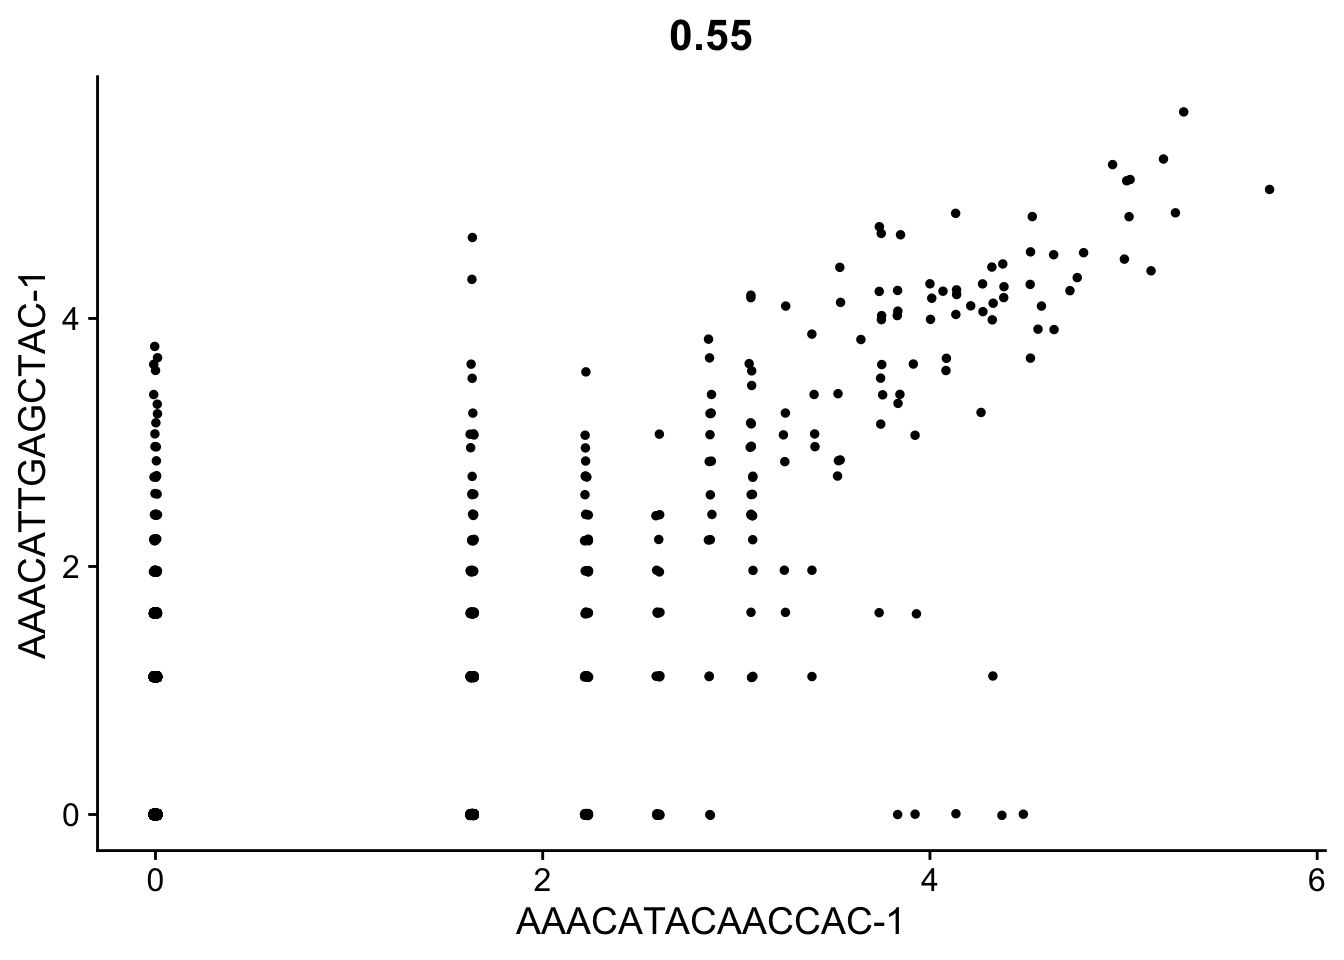
\includegraphics{scRNAseqInR_Doco_files/figure-latex/unnamed-chunk-30-1.pdf}

DotPlots

\begin{Shaded}
\begin{Highlighting}[]
\FunctionTok{DotPlot}\NormalTok{(pbmc, }\AttributeTok{features =} \FunctionTok{c}\NormalTok{(}\StringTok{"MS4A1"}\NormalTok{, }\StringTok{"GNLY"}\NormalTok{, }\StringTok{"CD3E"}\NormalTok{, }\StringTok{"CD14"}\NormalTok{, }\StringTok{"FCER1A"}\NormalTok{, }\StringTok{"FCGR3A"}\NormalTok{, }\StringTok{"LYZ"}\NormalTok{, }\StringTok{"PPBP"}\NormalTok{, }\StringTok{"CD8A"}\NormalTok{))}
\end{Highlighting}
\end{Shaded}

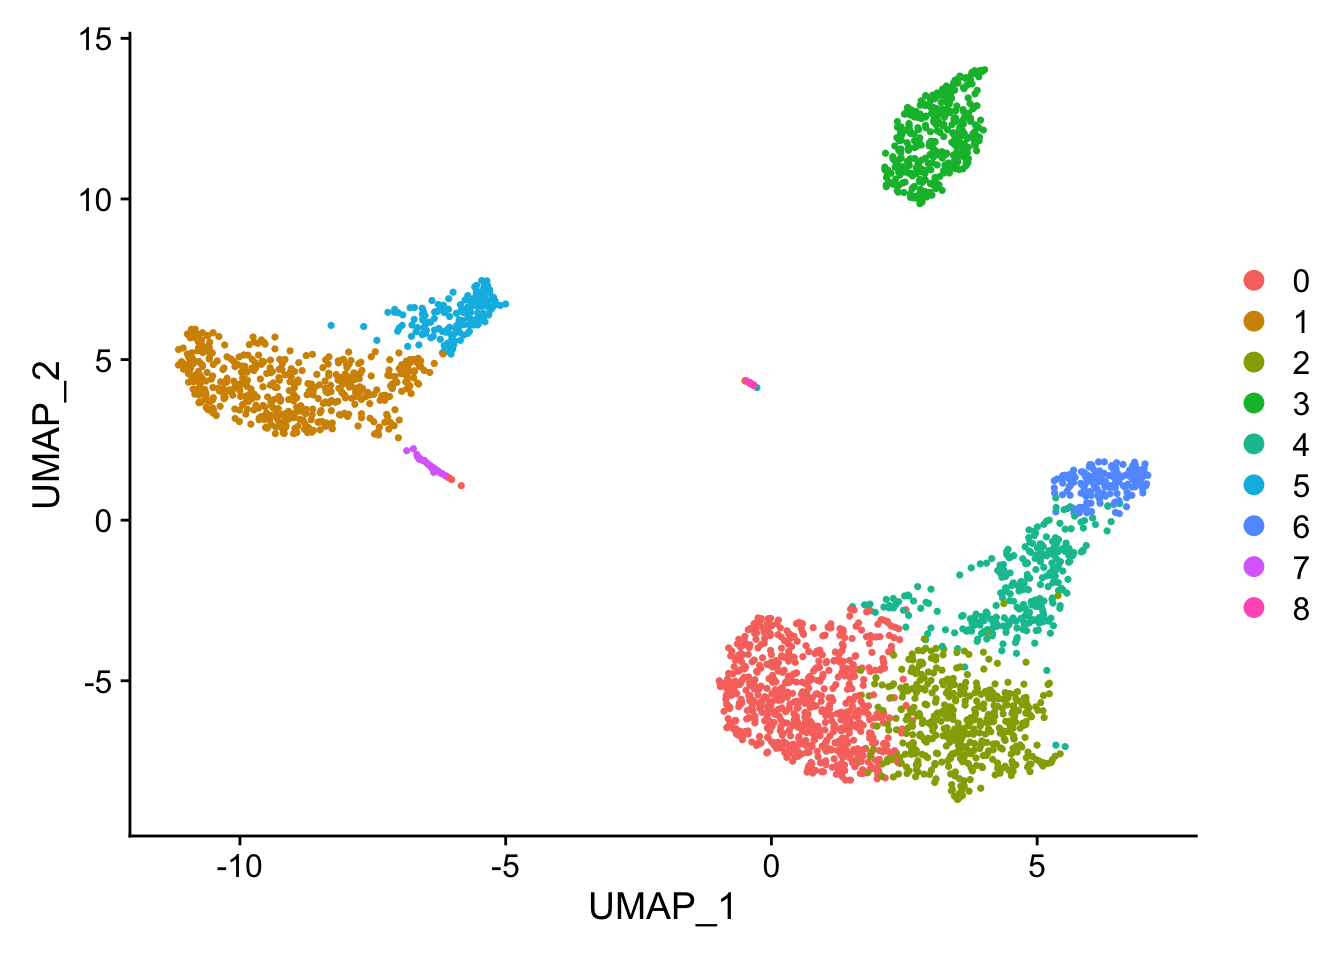
\includegraphics{scRNAseqInR_Doco_files/figure-latex/unnamed-chunk-31-1.pdf}

\texttt{DoHeatmap()} generates an expression heatmap for given cells and features. In this case, we are plotting the top 20 markers (or all markers if less than 20) for each cluster.

\begin{Shaded}
\begin{Highlighting}[]
\NormalTok{top10 }\OtherTok{\textless{}{-}}\NormalTok{ pbmc.markers }\SpecialCharTok{\%\textgreater{}\%} \FunctionTok{group\_by}\NormalTok{(cluster) }\SpecialCharTok{\%\textgreater{}\%} \FunctionTok{top\_n}\NormalTok{(}\AttributeTok{n =} \DecValTok{10}\NormalTok{, }\AttributeTok{wt =}\NormalTok{ avg\_log2FC)}
\FunctionTok{DoHeatmap}\NormalTok{(pbmc, }\AttributeTok{features =}\NormalTok{ top10}\SpecialCharTok{$}\NormalTok{gene) }\SpecialCharTok{+} \FunctionTok{NoLegend}\NormalTok{()}
\end{Highlighting}
\end{Shaded}

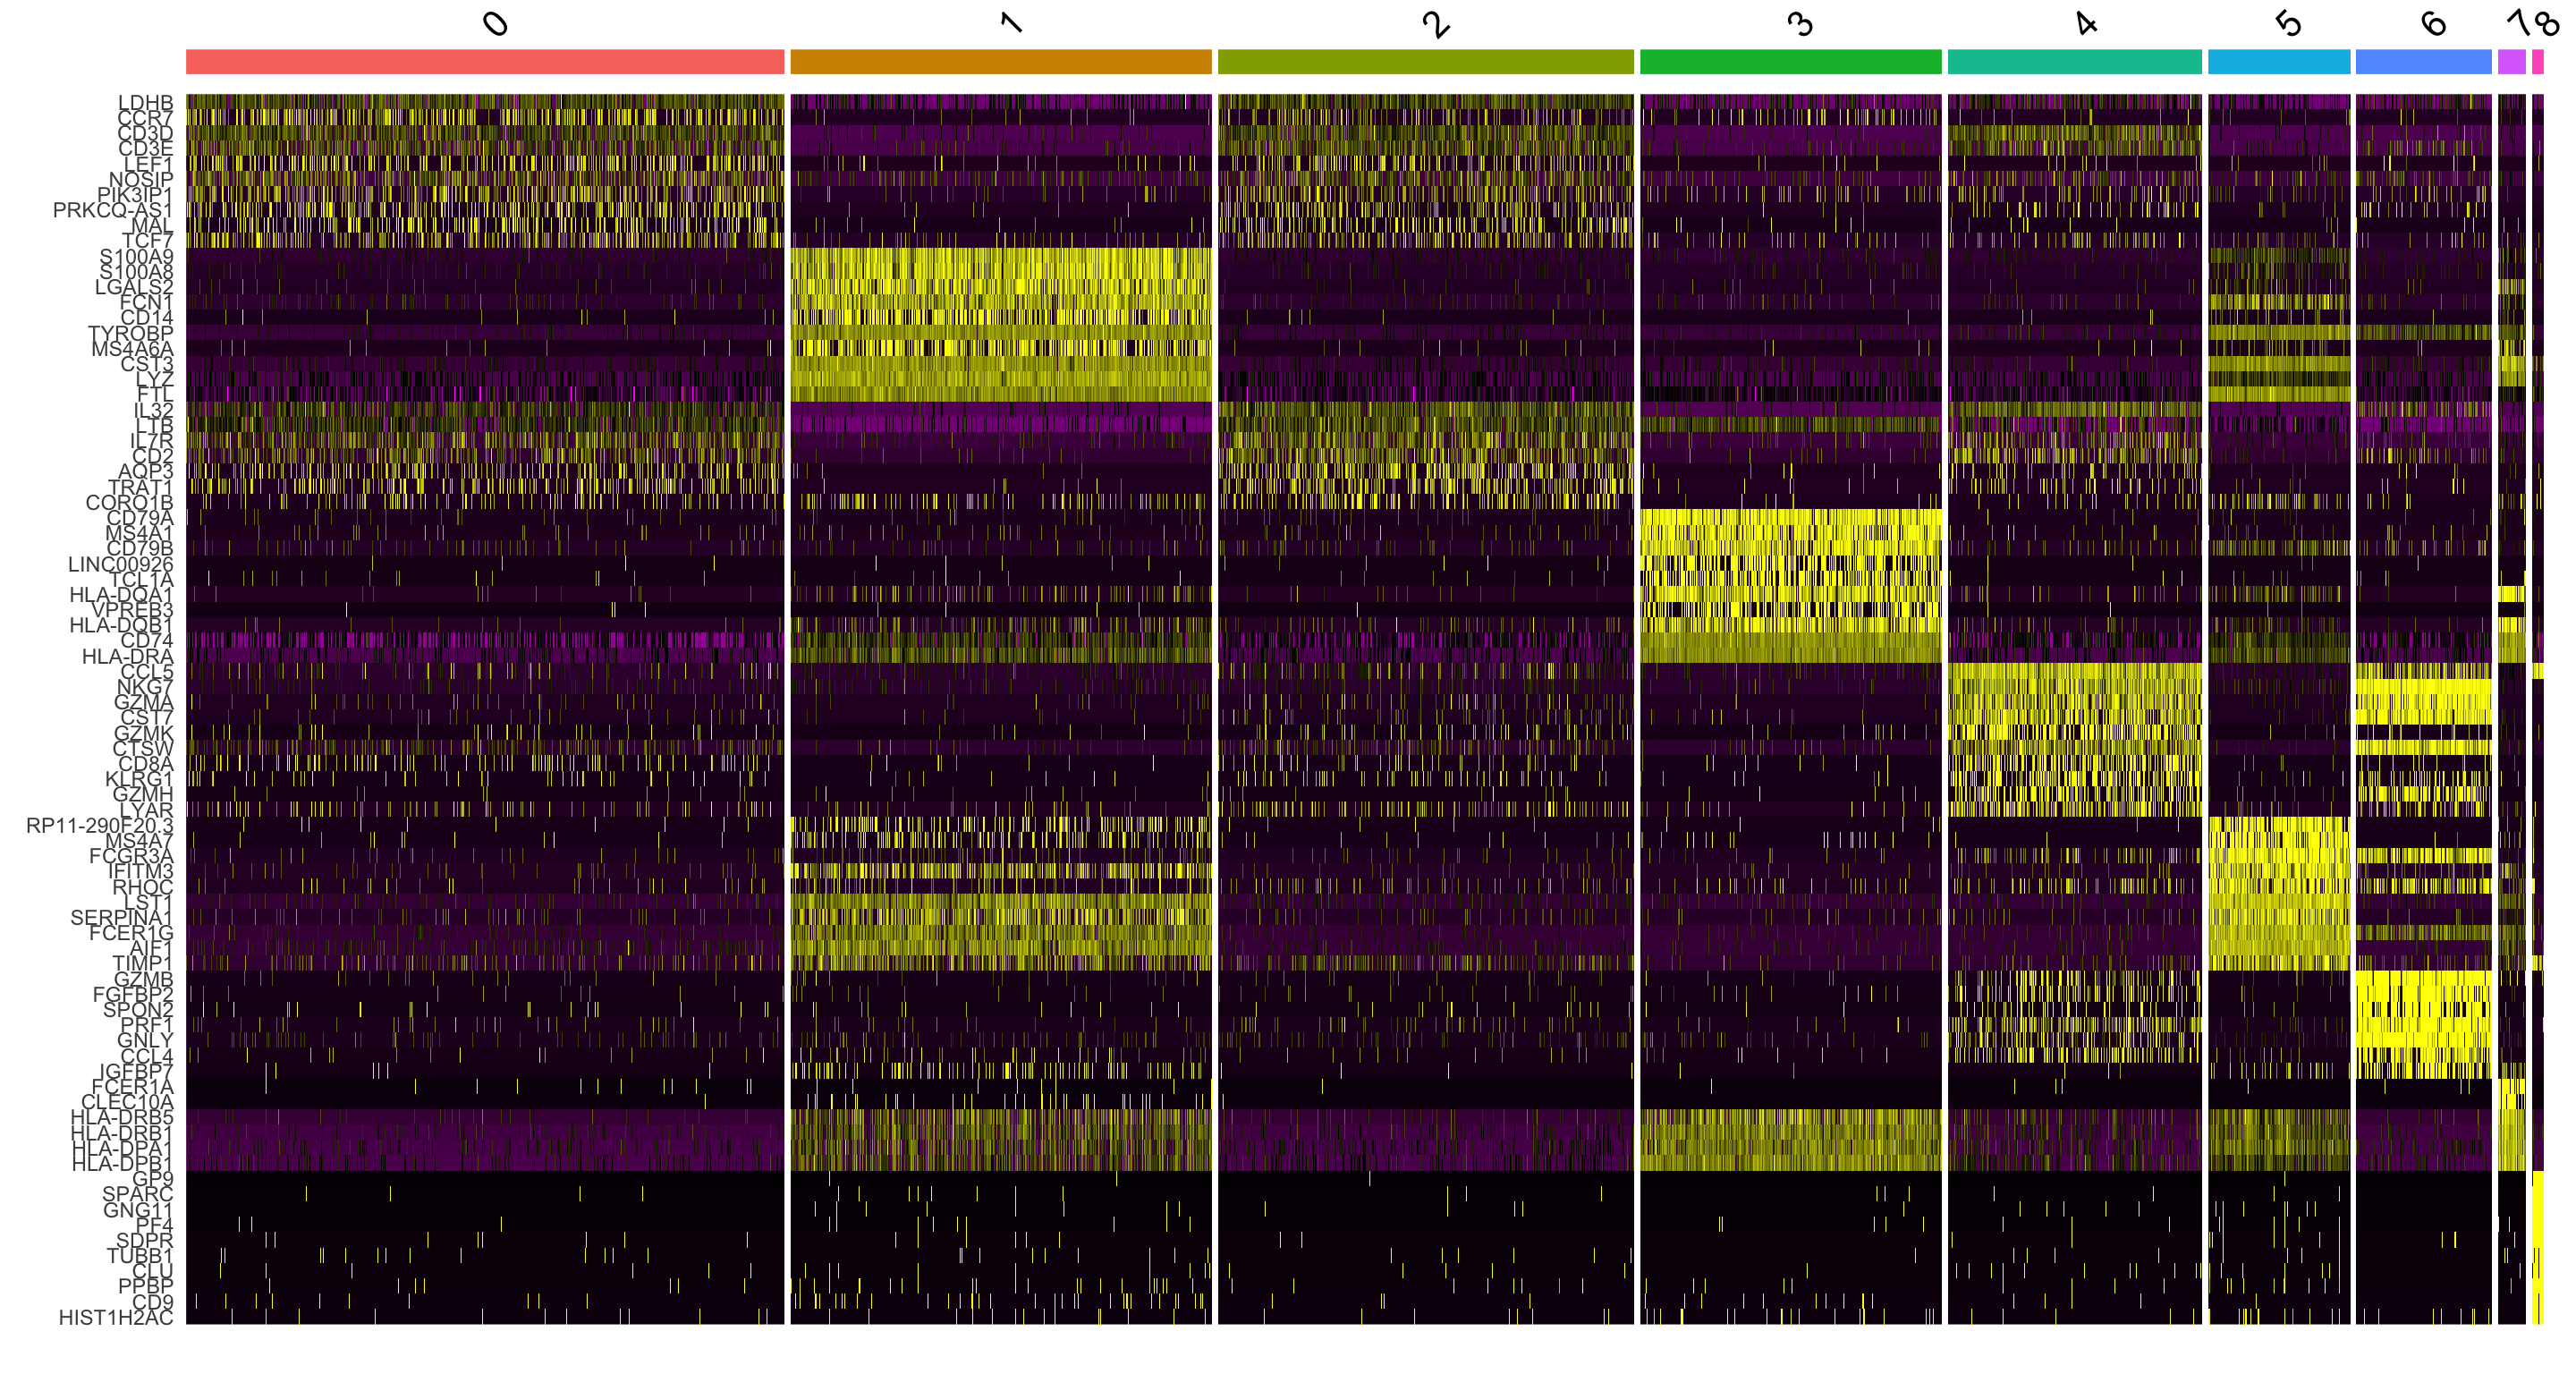
\includegraphics{scRNAseqInR_Doco_files/figure-latex/clusterHeatmap-1.pdf}

\hypertarget{use-makers-to-label-or-find-a-cluster}{%
\section{Use makers to label or find a cluster}\label{use-makers-to-label-or-find-a-cluster}}

If you know markers for your cell types, use AddModuleScore to label them.

\begin{Shaded}
\begin{Highlighting}[]
\NormalTok{genes\_markers }\OtherTok{\textless{}{-}} \FunctionTok{list}\NormalTok{(}\AttributeTok{Naive\_CD4\_T =} \FunctionTok{c}\NormalTok{(}\StringTok{"IL7R"}\NormalTok{, }\StringTok{"CCR7"}\NormalTok{))}

\NormalTok{pbmc }\OtherTok{\textless{}{-}} \FunctionTok{AddModuleScore}\NormalTok{(}\AttributeTok{object =}\NormalTok{ pbmc, }\AttributeTok{features =}\NormalTok{ genes\_markers, }\AttributeTok{ctrl =} \DecValTok{5}\NormalTok{, }\AttributeTok{name =} \StringTok{"Naive\_CD4\_T"}\NormalTok{,}
    \AttributeTok{search =} \ConstantTok{TRUE}\NormalTok{)}


\CommentTok{\# notice the name of the cluster has a 1 at the end}
\FunctionTok{names}\NormalTok{(pbmc}\SpecialCharTok{@}\NormalTok{meta.data)}
\CommentTok{\#\textgreater{}  [1] "orig.ident"      "nCount\_RNA"      "nFeature\_RNA"   }
\CommentTok{\#\textgreater{}  [4] "percent.mt"      "RNA\_snn\_res.0.5" "seurat\_clusters"}
\CommentTok{\#\textgreater{}  [7] "RNA\_snn\_res.0.1" "RNA\_snn\_res.0.2" "RNA\_snn\_res.0.3"}
\CommentTok{\#\textgreater{} [10] "RNA\_snn\_res.0.4" "RNA\_snn\_res.0.6" "RNA\_snn\_res.0.7"}
\CommentTok{\#\textgreater{} [13] "RNA\_snn\_res.0.8" "RNA\_snn\_res.0.9" "RNA\_snn\_res.1"  }
\CommentTok{\#\textgreater{} [16] "RNA\_snn\_res.1.1" "RNA\_snn\_res.1.2" "RNA\_snn\_res.1.3"}
\CommentTok{\#\textgreater{} [19] "RNA\_snn\_res.1.4" "RNA\_snn\_res.1.5" "RNA\_snn\_res.1.6"}
\CommentTok{\#\textgreater{} [22] "RNA\_snn\_res.1.7" "RNA\_snn\_res.1.8" "RNA\_snn\_res.1.9"}
\CommentTok{\#\textgreater{} [25] "RNA\_snn\_res.2"   "Naive\_CD4\_T1"}

\CommentTok{\# label that cell type}
\NormalTok{pbmc}\SpecialCharTok{$}\NormalTok{cell\_label }\OtherTok{=} \ConstantTok{NA}
\NormalTok{pbmc}\SpecialCharTok{$}\NormalTok{cell\_label[pbmc}\SpecialCharTok{$}\NormalTok{Naive\_CD4\_T1 }\SpecialCharTok{\textgreater{}} \DecValTok{1}\NormalTok{] }\OtherTok{=} \StringTok{"Naive\_CD4\_T"}
\FunctionTok{Idents}\NormalTok{(pbmc) }\OtherTok{=}\NormalTok{ pbmc}\SpecialCharTok{$}\NormalTok{cell\_label}

\CommentTok{\# plot}
\CommentTok{\# Using a custom colour scale }
\FunctionTok{FeaturePlot}\NormalTok{(pbmc, }\AttributeTok{features =} \StringTok{"Naive\_CD4\_T1"}\NormalTok{, }\AttributeTok{label =} \ConstantTok{TRUE}\NormalTok{, }\AttributeTok{repel =} \ConstantTok{TRUE}\NormalTok{, ) }\SpecialCharTok{+} \FunctionTok{scale\_colour\_gradientn}\NormalTok{(}\AttributeTok{colours =} \FunctionTok{c}\NormalTok{(}\StringTok{"lightblue"}\NormalTok{,}\StringTok{"beige"}\NormalTok{,}\StringTok{"red"}\NormalTok{))}
\CommentTok{\#\textgreater{} Scale for colour is already present.}
\CommentTok{\#\textgreater{} Adding another scale for colour, which will replace the}
\CommentTok{\#\textgreater{} existing scale.}
\end{Highlighting}
\end{Shaded}

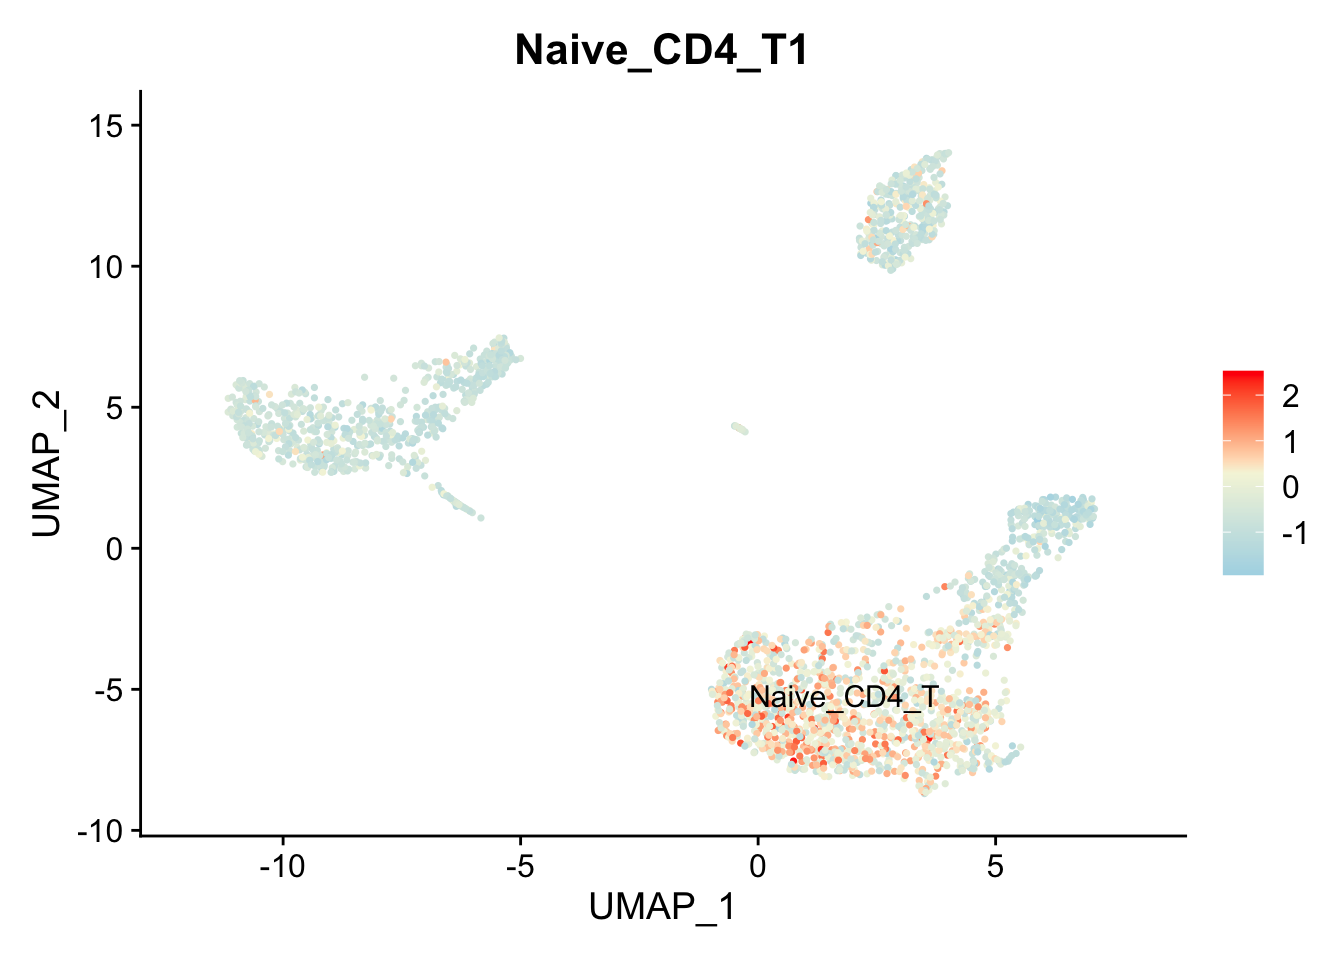
\includegraphics{scRNAseqInR_Doco_files/figure-latex/unnamed-chunk-32-1.pdf}

\hypertarget{assigning-cell-type-identity-to-clusters}{%
\section{Assigning cell type identity to clusters}\label{assigning-cell-type-identity-to-clusters}}

Fortunately in the case of this dataset, we can use canonical markers to easily match the unbiased clustering to known cell types:

\begin{longtable}[]{@{}lll@{}}
\toprule\noalign{}
Cluster ID & Markers & Cell Type \\
\midrule\noalign{}
\endhead
\bottomrule\noalign{}
\endlastfoot
0 & IL7R, CCR7 & Naive CD4+ T \\
1 & CD14, LYZ & CD14+ Mono \\
2 & IL7R, S100A4 & Memory CD4+ \\
3 & MS4A1 & B \\
4 & CD8A & CD8+ T \\
5 & FCGR3A, MS4A7 & FCGR3A+ Mono \\
6 & GNLY, NKG7 & NK \\
7 & FCER1A, CST3 & DC \\
8 & PPBP & Platelet \\
\end{longtable}

\begin{Shaded}
\begin{Highlighting}[]
\FunctionTok{Idents}\NormalTok{(pbmc) }\OtherTok{\textless{}{-}}\NormalTok{ pbmc}\SpecialCharTok{$}\NormalTok{RNA\_snn\_res.}\FloatTok{0.5}
\NormalTok{new.cluster.ids }\OtherTok{\textless{}{-}} \FunctionTok{c}\NormalTok{(}\StringTok{"Naive CD4 T"}\NormalTok{, }\StringTok{"CD14+ Mono"}\NormalTok{, }\StringTok{"Memory CD4 T"}\NormalTok{, }\StringTok{"B"}\NormalTok{, }\StringTok{"CD8 T"}\NormalTok{, }\StringTok{"FCGR3A+ Mono"}\NormalTok{, }\StringTok{"NK"}\NormalTok{, }\StringTok{"DC"}\NormalTok{, }\StringTok{"Platelet"}\NormalTok{)}
\FunctionTok{names}\NormalTok{(new.cluster.ids) }\OtherTok{\textless{}{-}} \FunctionTok{levels}\NormalTok{(pbmc)}
\NormalTok{pbmc }\OtherTok{\textless{}{-}} \FunctionTok{RenameIdents}\NormalTok{(pbmc, new.cluster.ids)}
\FunctionTok{DimPlot}\NormalTok{(pbmc, }\AttributeTok{reduction =} \StringTok{\textquotesingle{}umap\textquotesingle{}}\NormalTok{, }\AttributeTok{label =} \ConstantTok{TRUE}\NormalTok{, }\AttributeTok{pt.size =} \FloatTok{0.5}\NormalTok{) }\SpecialCharTok{+} \FunctionTok{NoLegend}\NormalTok{()}
\end{Highlighting}
\end{Shaded}

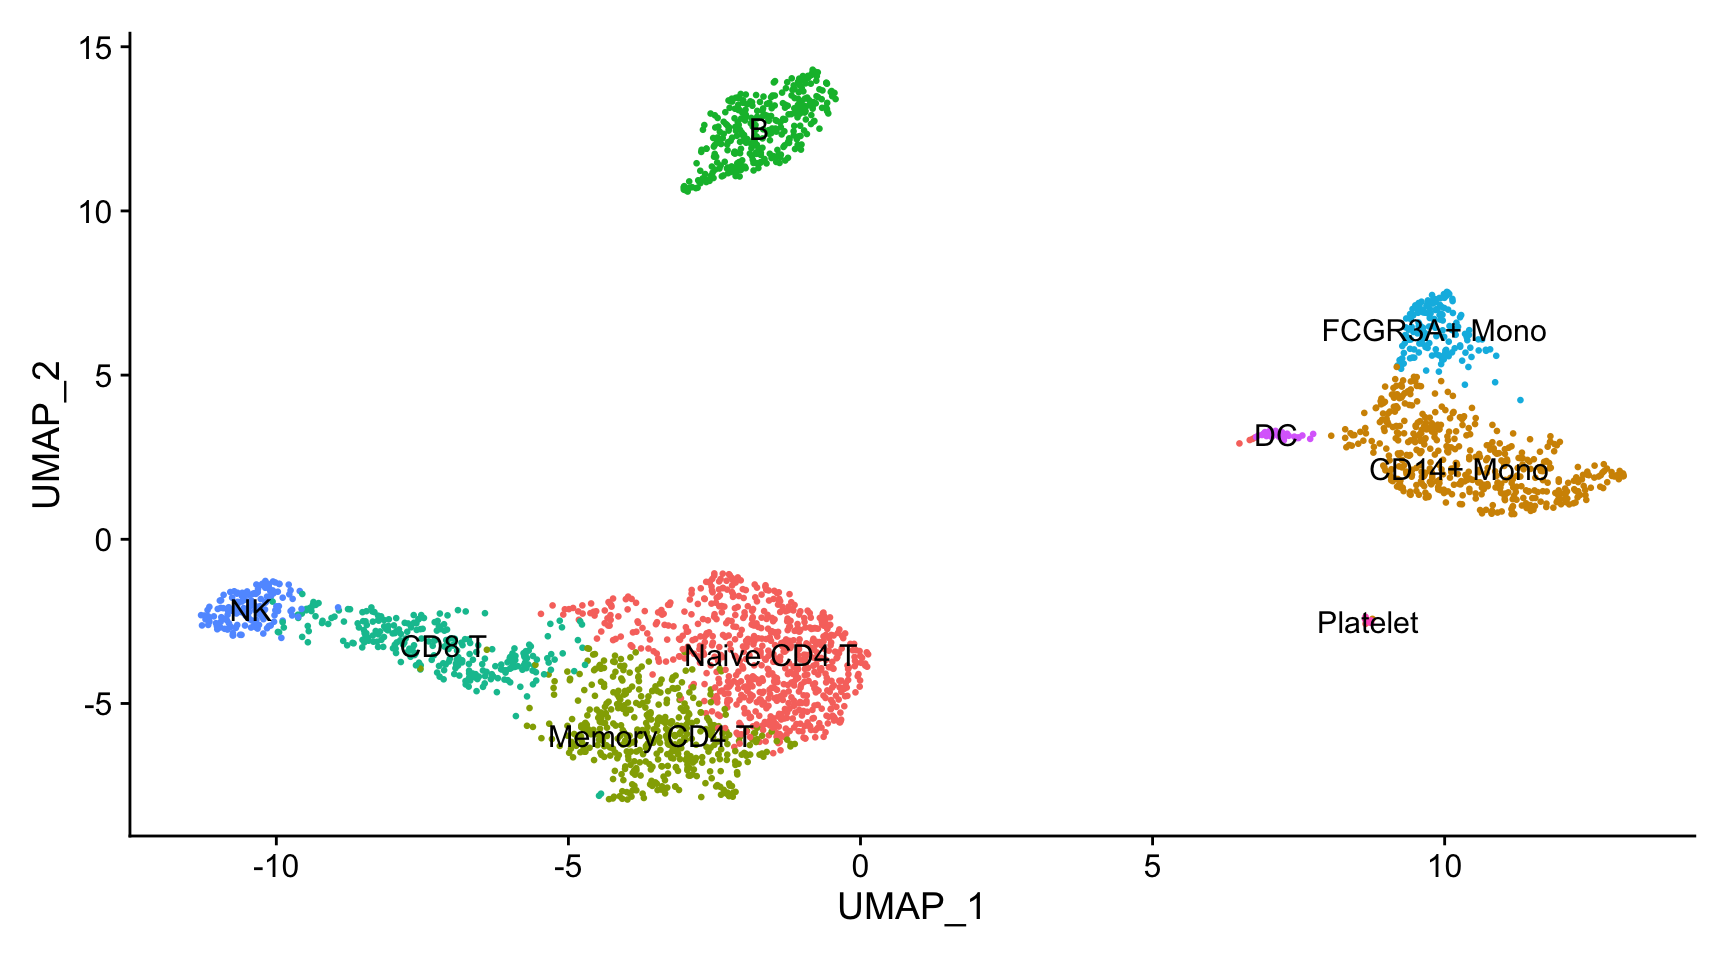
\includegraphics{scRNAseqInR_Doco_files/figure-latex/labelplot-1.pdf}

\begin{Shaded}
\begin{Highlighting}[]
\FunctionTok{saveRDS}\NormalTok{(pbmc, }\AttributeTok{file =} \StringTok{"pbmc3k\_final.rds"}\NormalTok{)}
\end{Highlighting}
\end{Shaded}

\hypertarget{part-futher-analysis}{%
\part{Futher Analysis}\label{part-futher-analysis}}

\hypertarget{singler}{%
\chapter{SingleR}\label{singler}}

\begin{Shaded}
\begin{Highlighting}[]
\CommentTok{\#install.packages("BiocManager")}
\CommentTok{\#BiocManager::install(c("SingleCellExperiment","SingleR","celldex"),ask=F)}
\FunctionTok{library}\NormalTok{(SingleCellExperiment)}
\FunctionTok{library}\NormalTok{(SingleR)}
\FunctionTok{library}\NormalTok{(celldex)}
\end{Highlighting}
\end{Shaded}

In this workshop we have focused on the Seurat package. However, there is another whole ecosystem of R packages for single cell analysis within Bioconductor. We won't go into any detail on these packages in this workshop, but there is good material describing the object type online : \href{https://robertamezquita.github.io/orchestratingSingleCellAnalysis/data-infrastructure.html}{OSCA}.

For now, we'll just convert our Seurat object into an object called SingleCellExperiment. Some popular packages from Bioconductor that work with this type are Slingshot, Scran, Scater.

\begin{Shaded}
\begin{Highlighting}[]
\NormalTok{sce }\OtherTok{\textless{}{-}} \FunctionTok{as.SingleCellExperiment}\NormalTok{(pbmc)}
\end{Highlighting}
\end{Shaded}

We will now use a package called SingleR to label each cell. SingleR uses a reference data set of cell types with expression data to infer the best label for each cell. A convenient collection of cell type reference is in the \texttt{celldex} package which currently contains the follow sets:

\begin{Shaded}
\begin{Highlighting}[]
\FunctionTok{ls}\NormalTok{(}\StringTok{\textquotesingle{}package:celldex\textquotesingle{}}\NormalTok{)}
\CommentTok{\#\textgreater{} [1] "BlueprintEncodeData"             }
\CommentTok{\#\textgreater{} [2] "DatabaseImmuneCellExpressionData"}
\CommentTok{\#\textgreater{} [3] "HumanPrimaryCellAtlasData"       }
\CommentTok{\#\textgreater{} [4] "ImmGenData"                      }
\CommentTok{\#\textgreater{} [5] "MonacoImmuneData"                }
\CommentTok{\#\textgreater{} [6] "MouseRNAseqData"                 }
\CommentTok{\#\textgreater{} [7] "NovershternHematopoieticData"}
\end{Highlighting}
\end{Shaded}

In this example, we'll use the \texttt{HumanPrimaryCellAtlasData} set, which contains high-level, and fine-grained label types. Lets download the reference dataset

\begin{Shaded}
\begin{Highlighting}[]
\NormalTok{ref.set }\OtherTok{\textless{}{-}}\NormalTok{ celldex}\SpecialCharTok{::}\FunctionTok{HumanPrimaryCellAtlasData}\NormalTok{()}
\CommentTok{\#\textgreater{} see ?celldex and browseVignettes(\textquotesingle{}celldex\textquotesingle{}) for documentation}
\CommentTok{\#\textgreater{} loading from cache}
\CommentTok{\#\textgreater{} see ?celldex and browseVignettes(\textquotesingle{}celldex\textquotesingle{}) for documentation}
\CommentTok{\#\textgreater{} loading from cache}
\FunctionTok{head}\NormalTok{(}\FunctionTok{unique}\NormalTok{(ref.set}\SpecialCharTok{$}\NormalTok{label.main))}
\CommentTok{\#\textgreater{} [1] "DC"                  "Smooth\_muscle\_cells"}
\CommentTok{\#\textgreater{} [3] "Epithelial\_cells"    "B\_cell"             }
\CommentTok{\#\textgreater{} [5] "Neutrophils"         "T\_cells"}
\end{Highlighting}
\end{Shaded}

An example of the types of ``fine'' labels.

\begin{Shaded}
\begin{Highlighting}[]
\FunctionTok{head}\NormalTok{(}\FunctionTok{unique}\NormalTok{(ref.set}\SpecialCharTok{$}\NormalTok{label.fine))}
\CommentTok{\#\textgreater{} [1] "DC:monocyte{-}derived:immature"       }
\CommentTok{\#\textgreater{} [2] "DC:monocyte{-}derived:Galectin{-}1"     }
\CommentTok{\#\textgreater{} [3] "DC:monocyte{-}derived:LPS"            }
\CommentTok{\#\textgreater{} [4] "DC:monocyte{-}derived"                }
\CommentTok{\#\textgreater{} [5] "Smooth\_muscle\_cells:bronchial:vit\_D"}
\CommentTok{\#\textgreater{} [6] "Smooth\_muscle\_cells:bronchial"}
\end{Highlighting}
\end{Shaded}

Now we'll label our cells using the SingleCellExperiment object, with the above reference set.

\begin{Shaded}
\begin{Highlighting}[]
\NormalTok{pred.cnts }\OtherTok{\textless{}{-}}\NormalTok{ SingleR}\SpecialCharTok{::}\FunctionTok{SingleR}\NormalTok{(}\AttributeTok{test =}\NormalTok{ sce, }\AttributeTok{ref =}\NormalTok{ ref.set, }\AttributeTok{labels =}\NormalTok{ ref.set}\SpecialCharTok{$}\NormalTok{label.main)}
\end{Highlighting}
\end{Shaded}

Keep any types that have more than 10 cells to the label, and put those labels back on our Seurat object and plot our on our umap.

\begin{Shaded}
\begin{Highlighting}[]
\NormalTok{lbls.keep }\OtherTok{\textless{}{-}} \FunctionTok{table}\NormalTok{(pred.cnts}\SpecialCharTok{$}\NormalTok{labels)}\SpecialCharTok{\textgreater{}}\DecValTok{10}
\NormalTok{pbmc}\SpecialCharTok{$}\NormalTok{SingleR.labels }\OtherTok{\textless{}{-}} \FunctionTok{ifelse}\NormalTok{(lbls.keep[pred.cnts}\SpecialCharTok{$}\NormalTok{labels], pred.cnts}\SpecialCharTok{$}\NormalTok{labels, }\StringTok{\textquotesingle{}Other\textquotesingle{}}\NormalTok{)}
\FunctionTok{DimPlot}\NormalTok{(pbmc, }\AttributeTok{reduction=}\StringTok{\textquotesingle{}umap\textquotesingle{}}\NormalTok{, }\AttributeTok{group.by=}\StringTok{\textquotesingle{}SingleR.labels\textquotesingle{}}\NormalTok{)}
\end{Highlighting}
\end{Shaded}

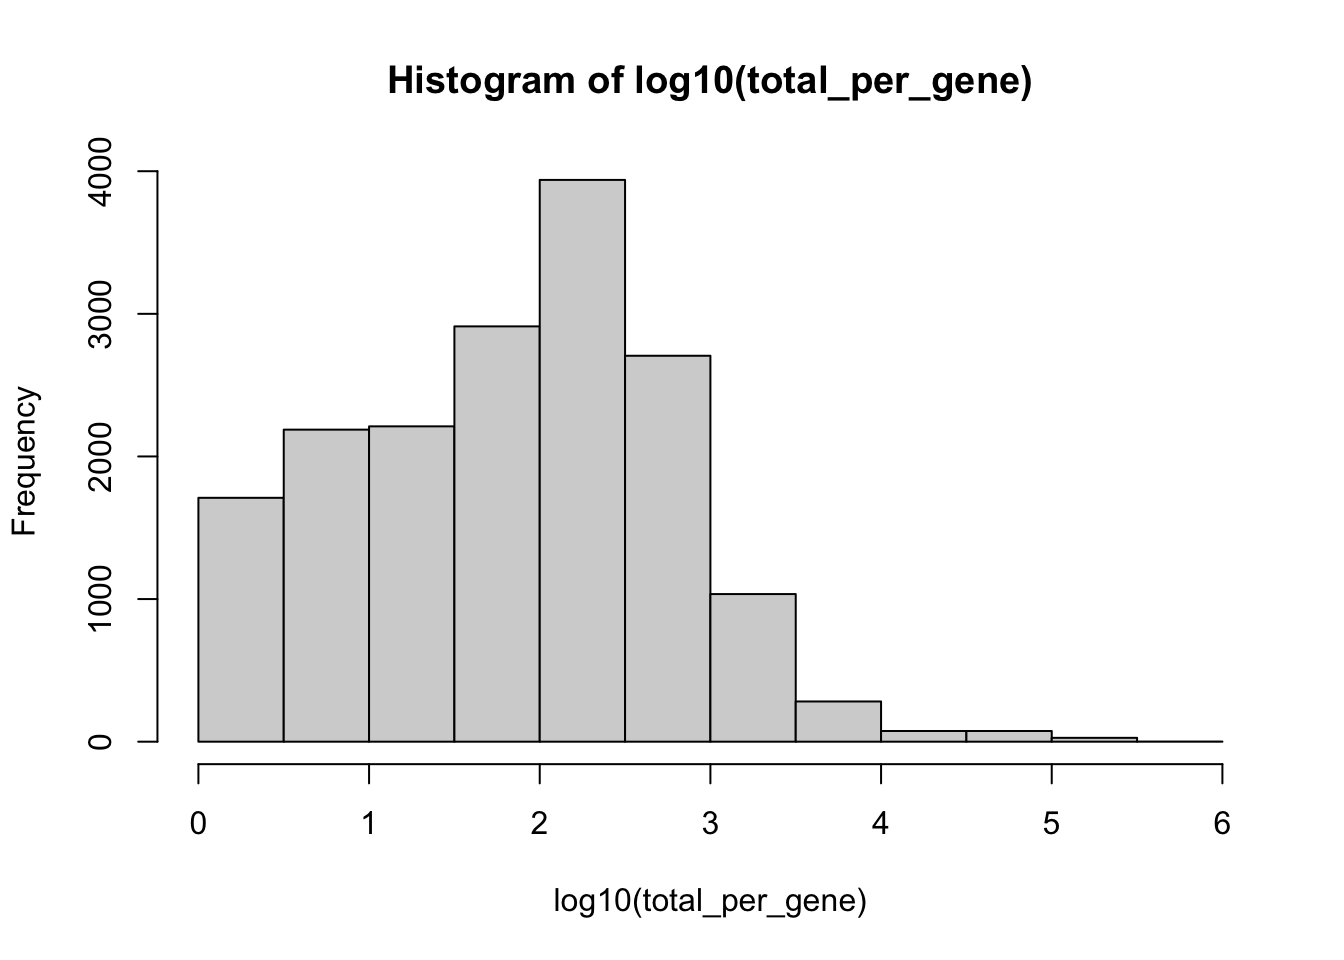
\includegraphics{scRNAseqInR_Doco_files/figure-latex/unnamed-chunk-40-1.pdf}

It is nice to see that even though SingleR does not use the clusters we computed earlier, the labels do seem to match those clusters reasonably well.

\hypertarget{de2}{%
\chapter{Differential Expression}\label{de2}}

There are many different methods for calculating differential expression between groups in scRNAseq data. There are a number of review papers worth consulting on this topic.

There is the \href{https://satijalab.org/seurat/archive/v3.1/de_vignette.html}{Seurat differential expression Vignette} which walks through the variety implemented in Seurat.

There is also a good
This includes a good discussion of useing \href{http://bioconductor.org/books/3.15/OSCA.multisample/multi-sample-comparisons.html\#creating-pseudo-bulk-samples}{pseudobulk approaches}, worth checking out for differential expression analyses.

The example below quickly looks at 3 different methods on the Kang 2018 PBMC dataset \ldots.

We will now look at \href{https://www.ncbi.nlm.nih.gov/geo/query/acc.cgi?acc=GSE96583}{GSE96583}, another PBMC dataset. For speed, we will be looking at a subset of 5000 cells from this data. The cells in this dataset were pooled from eight individual donors. A nice feature is that genetic differences allow some of the cell doublets to be identified. This data contains two batches of single cell sequencing. One of the batches was stimulated with IFN-beta.

The data has already been processed as we have done with the first PBMC dataset, and can be loaded from \texttt{kang2018.rds}.

\begin{Shaded}
\begin{Highlighting}[]
\NormalTok{kang }\OtherTok{\textless{}{-}} \FunctionTok{readRDS}\NormalTok{(}\StringTok{"data/kang2018.rds"}\NormalTok{)}
\FunctionTok{head}\NormalTok{(kang}\SpecialCharTok{@}\NormalTok{meta.data)}
\CommentTok{\#\textgreater{}                     orig.ident nCount\_RNA nFeature\_RNA  ind}
\CommentTok{\#\textgreater{} AGGGCGCTATTTCC{-}1 SeuratProject       2020          523 1256}
\CommentTok{\#\textgreater{} GGAGACGATTCGTT{-}1 SeuratProject        840          381 1256}
\CommentTok{\#\textgreater{} CACCGTTGTCGTAG{-}1 SeuratProject       3097          995 1016}
\CommentTok{\#\textgreater{} TATCGTACACGCAT{-}1 SeuratProject       1011          540 1488}
\CommentTok{\#\textgreater{} TGACGCCTTGCTTT{-}1 SeuratProject        570          367  101}
\CommentTok{\#\textgreater{} TACGAGACCTATTC{-}1 SeuratProject       2399          770 1244}
\CommentTok{\#\textgreater{}                  stim              cell multiplets}
\CommentTok{\#\textgreater{} AGGGCGCTATTTCC{-}1 stim   CD14+ Monocytes    singlet}
\CommentTok{\#\textgreater{} GGAGACGATTCGTT{-}1 stim       CD4 T cells    singlet}
\CommentTok{\#\textgreater{} CACCGTTGTCGTAG{-}1 ctrl FCGR3A+ Monocytes    singlet}
\CommentTok{\#\textgreater{} TATCGTACACGCAT{-}1 stim           B cells    singlet}
\CommentTok{\#\textgreater{} TGACGCCTTGCTTT{-}1 ctrl       CD4 T cells       ambs}
\CommentTok{\#\textgreater{} TACGAGACCTATTC{-}1 stim       CD4 T cells    singlet}
\end{Highlighting}
\end{Shaded}

How cells from each condition do we have?

\begin{Shaded}
\begin{Highlighting}[]
\FunctionTok{table}\NormalTok{(kang}\SpecialCharTok{$}\NormalTok{stim)}
\CommentTok{\#\textgreater{} }
\CommentTok{\#\textgreater{} ctrl stim }
\CommentTok{\#\textgreater{} 2449 2551}
\end{Highlighting}
\end{Shaded}

How many cells per individuals per group?

\begin{Shaded}
\begin{Highlighting}[]
\FunctionTok{table}\NormalTok{(kang}\SpecialCharTok{$}\NormalTok{ind, kang}\SpecialCharTok{$}\NormalTok{stim)}
\CommentTok{\#\textgreater{}       }
\CommentTok{\#\textgreater{}        ctrl stim}
\CommentTok{\#\textgreater{}   101   178  229}
\CommentTok{\#\textgreater{}   107   117  107}
\CommentTok{\#\textgreater{}   1015  514  496}
\CommentTok{\#\textgreater{}   1016  356  356}
\CommentTok{\#\textgreater{}   1039  100  118}
\CommentTok{\#\textgreater{}   1244  380  313}
\CommentTok{\#\textgreater{}   1256  394  390}
\CommentTok{\#\textgreater{}   1488  410  542}
\end{Highlighting}
\end{Shaded}

And for each individual, how many of each cell type has been classified?

\begin{Shaded}
\begin{Highlighting}[]
\FunctionTok{table}\NormalTok{(}\FunctionTok{paste}\NormalTok{(kang}\SpecialCharTok{$}\NormalTok{ind,kang}\SpecialCharTok{$}\NormalTok{stim), kang}\SpecialCharTok{$}\NormalTok{cell)}
\CommentTok{\#\textgreater{}            }
\CommentTok{\#\textgreater{}             B cells CD14+ Monocytes CD4 T cells CD8 T cells}
\CommentTok{\#\textgreater{}   101 ctrl       24              48          61          15}
\CommentTok{\#\textgreater{}   101 stim       30              52          84          17}
\CommentTok{\#\textgreater{}   1015 ctrl      81             149         145          46}
\CommentTok{\#\textgreater{}   1015 stim      68             151         150          22}
\CommentTok{\#\textgreater{}   1016 ctrl      22              72          89         112}
\CommentTok{\#\textgreater{}   1016 stim      29              65          66         115}
\CommentTok{\#\textgreater{}   1039 ctrl       7              35          40           6}
\CommentTok{\#\textgreater{}   1039 stim       7              28          51           6}
\CommentTok{\#\textgreater{}   107 ctrl        9              51          32           6}
\CommentTok{\#\textgreater{}   107 stim        9              35          43           1}
\CommentTok{\#\textgreater{}   1244 ctrl      23              86         206           8}
\CommentTok{\#\textgreater{}   1244 stim      18              58         191           4}
\CommentTok{\#\textgreater{}   1256 ctrl      32              81         180          29}
\CommentTok{\#\textgreater{}   1256 stim      42              70         198          25}
\CommentTok{\#\textgreater{}   1488 ctrl      36              59         247          13}
\CommentTok{\#\textgreater{}   1488 stim      59              59         325          15}
\CommentTok{\#\textgreater{}            }
\CommentTok{\#\textgreater{}             Dendritic cells FCGR3A+ Monocytes}
\CommentTok{\#\textgreater{}   101 ctrl                4                11}
\CommentTok{\#\textgreater{}   101 stim                6                23}
\CommentTok{\#\textgreater{}   1015 ctrl               4                50}
\CommentTok{\#\textgreater{}   1015 stim              17                44}
\CommentTok{\#\textgreater{}   1016 ctrl               4                22}
\CommentTok{\#\textgreater{}   1016 stim               2                32}
\CommentTok{\#\textgreater{}   1039 ctrl               1                 3}
\CommentTok{\#\textgreater{}   1039 stim               1                 8}
\CommentTok{\#\textgreater{}   107 ctrl                3                12}
\CommentTok{\#\textgreater{}   107 stim                2                 5}
\CommentTok{\#\textgreater{}   1244 ctrl               8                19}
\CommentTok{\#\textgreater{}   1244 stim               6                 4}
\CommentTok{\#\textgreater{}   1256 ctrl               6                20}
\CommentTok{\#\textgreater{}   1256 stim               3                11}
\CommentTok{\#\textgreater{}   1488 ctrl               8                25}
\CommentTok{\#\textgreater{}   1488 stim              12                28}
\CommentTok{\#\textgreater{}            }
\CommentTok{\#\textgreater{}             Megakaryocytes NK cells}
\CommentTok{\#\textgreater{}   101 ctrl               4       11}
\CommentTok{\#\textgreater{}   101 stim               1       16}
\CommentTok{\#\textgreater{}   1015 ctrl              5       34}
\CommentTok{\#\textgreater{}   1015 stim              5       39}
\CommentTok{\#\textgreater{}   1016 ctrl              4       31}
\CommentTok{\#\textgreater{}   1016 stim              1       46}
\CommentTok{\#\textgreater{}   1039 ctrl              6        1}
\CommentTok{\#\textgreater{}   1039 stim             10        5}
\CommentTok{\#\textgreater{}   107 ctrl               1        3}
\CommentTok{\#\textgreater{}   107 stim               0       12}
\CommentTok{\#\textgreater{}   1244 ctrl              5       25}
\CommentTok{\#\textgreater{}   1244 stim              4       28}
\CommentTok{\#\textgreater{}   1256 ctrl              1       45}
\CommentTok{\#\textgreater{}   1256 stim              8       33}
\CommentTok{\#\textgreater{}   1488 ctrl              4       18}
\CommentTok{\#\textgreater{}   1488 stim              6       38}
\end{Highlighting}
\end{Shaded}

\hypertarget{prefiltering}{%
\section{Prefiltering}\label{prefiltering}}

When doing differential expression, you generally ignore genes with low experssion.
If expression is below a certain level, it will be almost impossible to see differential expression.

In single cell datasets, there are many genes like this. Filtering here to make our dataset smaller so it runs quicker, and there is less agressive correction for multiple hypotheses.

How many genes originally?

\begin{Shaded}
\begin{Highlighting}[]
\NormalTok{kang}
\CommentTok{\#\textgreater{} An object of class Seurat }
\CommentTok{\#\textgreater{} 35635 features across 5000 samples within 1 assay }
\CommentTok{\#\textgreater{} Active assay: RNA (35635 features, 2000 variable features)}
\CommentTok{\#\textgreater{}  2 dimensional reductions calculated: pca, umap}
\end{Highlighting}
\end{Shaded}

\begin{Shaded}
\begin{Highlighting}[]
\NormalTok{total\_per\_gene }\OtherTok{\textless{}{-}} \FunctionTok{rowSums}\NormalTok{(}\FunctionTok{GetAssayData}\NormalTok{(kang, }\StringTok{\textquotesingle{}counts\textquotesingle{}}\NormalTok{))}
\FunctionTok{hist}\NormalTok{(}\FunctionTok{log10}\NormalTok{(total\_per\_gene))}
\end{Highlighting}
\end{Shaded}

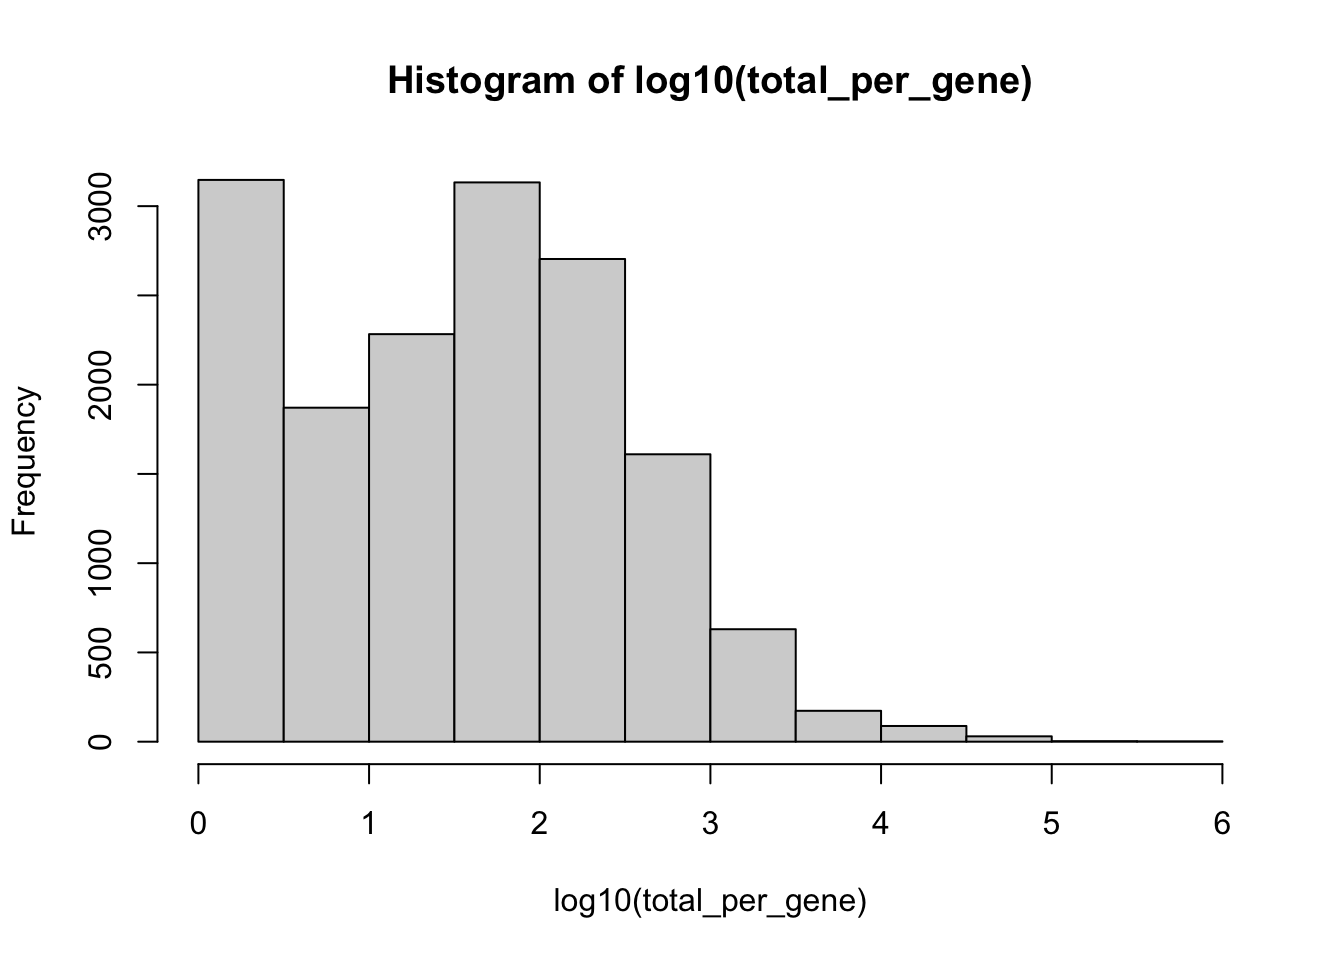
\includegraphics{scRNAseqInR_Doco_files/figure-latex/unnamed-chunk-47-1.pdf}

\begin{Shaded}
\begin{Highlighting}[]
\NormalTok{kang }\OtherTok{\textless{}{-}}\NormalTok{ kang[total\_per\_gene }\SpecialCharTok{\textgreater{}=} \DecValTok{50}\NormalTok{, ] }
\end{Highlighting}
\end{Shaded}

How many genes now?

\begin{Shaded}
\begin{Highlighting}[]
\NormalTok{kang}
\CommentTok{\#\textgreater{} An object of class Seurat }
\CommentTok{\#\textgreater{} 7216 features across 5000 samples within 1 assay }
\CommentTok{\#\textgreater{} Active assay: RNA (7216 features, 1228 variable features)}
\CommentTok{\#\textgreater{}  2 dimensional reductions calculated: pca, umap}
\end{Highlighting}
\end{Shaded}

We might like to see the effect of IFN-beta stimulation on each cell type individually. For the purpopses of this workshop, just going to test one cell type; CD14+ Monocytes

An easy way is to subset the object.

\begin{Shaded}
\begin{Highlighting}[]
\CommentTok{\# Set idents to \textquotesingle{}cell\textquotesingle{} column.}
\FunctionTok{Idents}\NormalTok{(kang) }\OtherTok{\textless{}{-}}\NormalTok{ kang}\SpecialCharTok{$}\NormalTok{cell}
\NormalTok{kang.celltype }\OtherTok{\textless{}{-}}\NormalTok{ kang[, kang}\SpecialCharTok{$}\NormalTok{cell }\SpecialCharTok{==} \StringTok{"CD14+ Monocytes"}\NormalTok{ ]}
\FunctionTok{DimPlot}\NormalTok{(kang) }\SpecialCharTok{+} \FunctionTok{DimPlot}\NormalTok{(kang.celltype)}
\end{Highlighting}
\end{Shaded}

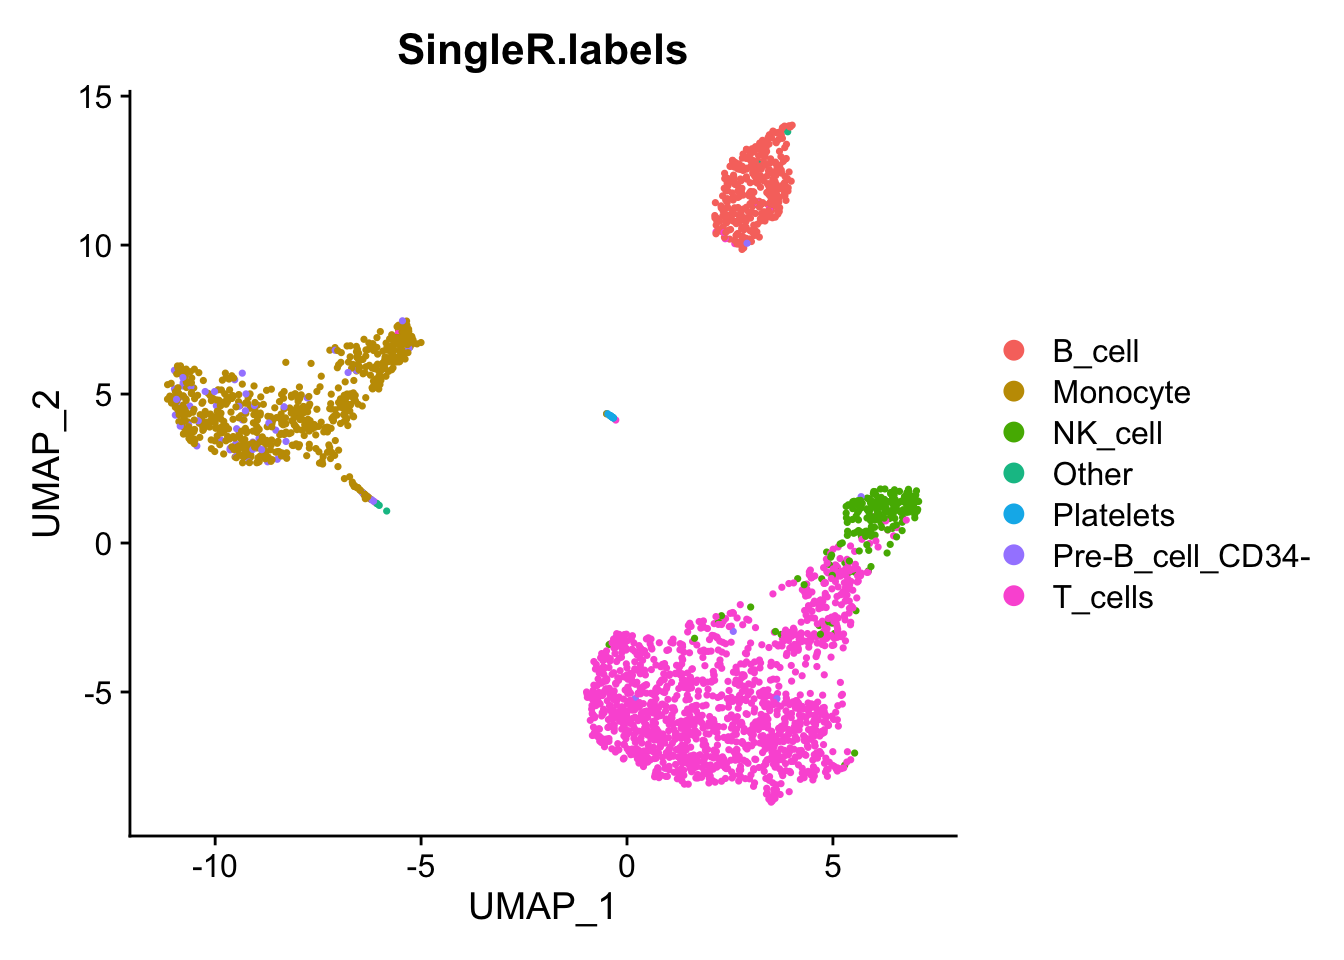
\includegraphics{scRNAseqInR_Doco_files/figure-latex/unnamed-chunk-49-1.pdf}

\hypertarget{default-wilcox-test}{%
\section{Default Wilcox test}\label{default-wilcox-test}}

To run this test, we change the Idents to the factor(column) we want to test. In this case, thats `stim'.

\begin{Shaded}
\begin{Highlighting}[]
\CommentTok{\# Change Ident to Condition}
\FunctionTok{Idents}\NormalTok{(kang.celltype) }\OtherTok{\textless{}{-}}\NormalTok{ kang.celltype}\SpecialCharTok{$}\NormalTok{stim}

\CommentTok{\# default, wilcox test}
\NormalTok{de\_result\_wilcox }\OtherTok{\textless{}{-}} \FunctionTok{FindMarkers}\NormalTok{(kang.celltype, }
            \AttributeTok{ident.1 =} \StringTok{\textquotesingle{}stim\textquotesingle{}}\NormalTok{,}
            \AttributeTok{ident.2 =} \StringTok{\textquotesingle{}ctrl\textquotesingle{}}\NormalTok{,}
            \AttributeTok{logfc.threshold =} \DecValTok{0}\NormalTok{, }\CommentTok{\# Give me ALL results}
            \AttributeTok{min.pct =} \DecValTok{0}
\NormalTok{            )}

\CommentTok{\# Add average expression for plotting}
\NormalTok{de\_result\_wilcox}\SpecialCharTok{$}\NormalTok{AveExpr}\OtherTok{\textless{}{-}} \FunctionTok{rowMeans}\NormalTok{(kang.celltype[[}\StringTok{"RNA"}\NormalTok{]][}\FunctionTok{rownames}\NormalTok{(de\_result\_wilcox),])}
\end{Highlighting}
\end{Shaded}

Look at the top differentially expressed genes.

\begin{Shaded}
\begin{Highlighting}[]
\FunctionTok{head}\NormalTok{(de\_result\_wilcox)}
\CommentTok{\#\textgreater{}                 p\_val avg\_log2FC pct.1 pct.2     p\_val\_adj}
\CommentTok{\#\textgreater{} RSAD2   5.541857e{-}197   4.928403 0.975 0.043 3.999004e{-}193}
\CommentTok{\#\textgreater{} CXCL10  9.648067e{-}197   6.963650 0.973 0.038 6.962045e{-}193}
\CommentTok{\#\textgreater{} IFIT3   4.988121e{-}196   4.736979 0.979 0.050 3.599428e{-}192}
\CommentTok{\#\textgreater{} TNFSF10 1.116418e{-}195   4.847351 0.977 0.055 8.056075e{-}192}
\CommentTok{\#\textgreater{} IFIT1   8.116699e{-}190   4.766009 0.950 0.026 5.857010e{-}186}
\CommentTok{\#\textgreater{} ISG15   1.524836e{-}187   6.143242 0.998 0.320 1.100322e{-}183}
\CommentTok{\#\textgreater{}          AveExpr}
\CommentTok{\#\textgreater{} RSAD2   1.686530}
\CommentTok{\#\textgreater{} CXCL10  2.388462}
\CommentTok{\#\textgreater{} IFIT3   1.701247}
\CommentTok{\#\textgreater{} TNFSF10 1.682688}
\CommentTok{\#\textgreater{} IFIT1   1.584751}
\CommentTok{\#\textgreater{} ISG15   3.239774}
\end{Highlighting}
\end{Shaded}

\begin{Shaded}
\begin{Highlighting}[]
\NormalTok{p1 }\OtherTok{\textless{}{-}} \FunctionTok{ggplot}\NormalTok{(de\_result\_wilcox, }\FunctionTok{aes}\NormalTok{(}\AttributeTok{x=}\NormalTok{AveExpr, }\AttributeTok{y=}\NormalTok{avg\_log2FC, }\AttributeTok{col=}\NormalTok{p\_val\_adj }\SpecialCharTok{\textless{}} \FloatTok{0.05}\NormalTok{)) }\SpecialCharTok{+}
  \FunctionTok{geom\_point}\NormalTok{() }\SpecialCharTok{+}
  \FunctionTok{scale\_colour\_manual}\NormalTok{(}\AttributeTok{values=}\FunctionTok{c}\NormalTok{(}\StringTok{\textquotesingle{}TRUE\textquotesingle{}}\OtherTok{=}\StringTok{"red"}\NormalTok{,}\StringTok{\textquotesingle{}FALSE\textquotesingle{}}\OtherTok{=}\StringTok{"black"}\NormalTok{)) }\SpecialCharTok{+} 
  \FunctionTok{theme\_bw}\NormalTok{() }\SpecialCharTok{+}
  \FunctionTok{ggtitle}\NormalTok{(}\StringTok{"Wilcox Test"}\NormalTok{)}


\NormalTok{p2 }\OtherTok{\textless{}{-}} \FunctionTok{ggplot}\NormalTok{(de\_result\_wilcox, }\FunctionTok{aes}\NormalTok{(}\AttributeTok{x=}\NormalTok{avg\_log2FC, }\AttributeTok{y=}\SpecialCharTok{{-}}\FunctionTok{log10}\NormalTok{(p\_val), }\AttributeTok{col=}\NormalTok{p\_val\_adj }\SpecialCharTok{\textless{}} \FloatTok{0.05}\NormalTok{)) }\SpecialCharTok{+}
  \FunctionTok{geom\_point}\NormalTok{() }\SpecialCharTok{+}
  \FunctionTok{scale\_colour\_manual}\NormalTok{(}\AttributeTok{values=}\FunctionTok{c}\NormalTok{(}\StringTok{\textquotesingle{}TRUE\textquotesingle{}}\OtherTok{=}\StringTok{"red"}\NormalTok{,}\StringTok{\textquotesingle{}FALSE\textquotesingle{}}\OtherTok{=}\StringTok{"black"}\NormalTok{)) }\SpecialCharTok{+} 
  \FunctionTok{theme\_bw}\NormalTok{() }\SpecialCharTok{+}
  \FunctionTok{ggtitle}\NormalTok{(}\StringTok{"Wilcox Test (Volcano)"}\NormalTok{)}

\NormalTok{p1 }\SpecialCharTok{+}\NormalTok{ p2}
\end{Highlighting}
\end{Shaded}

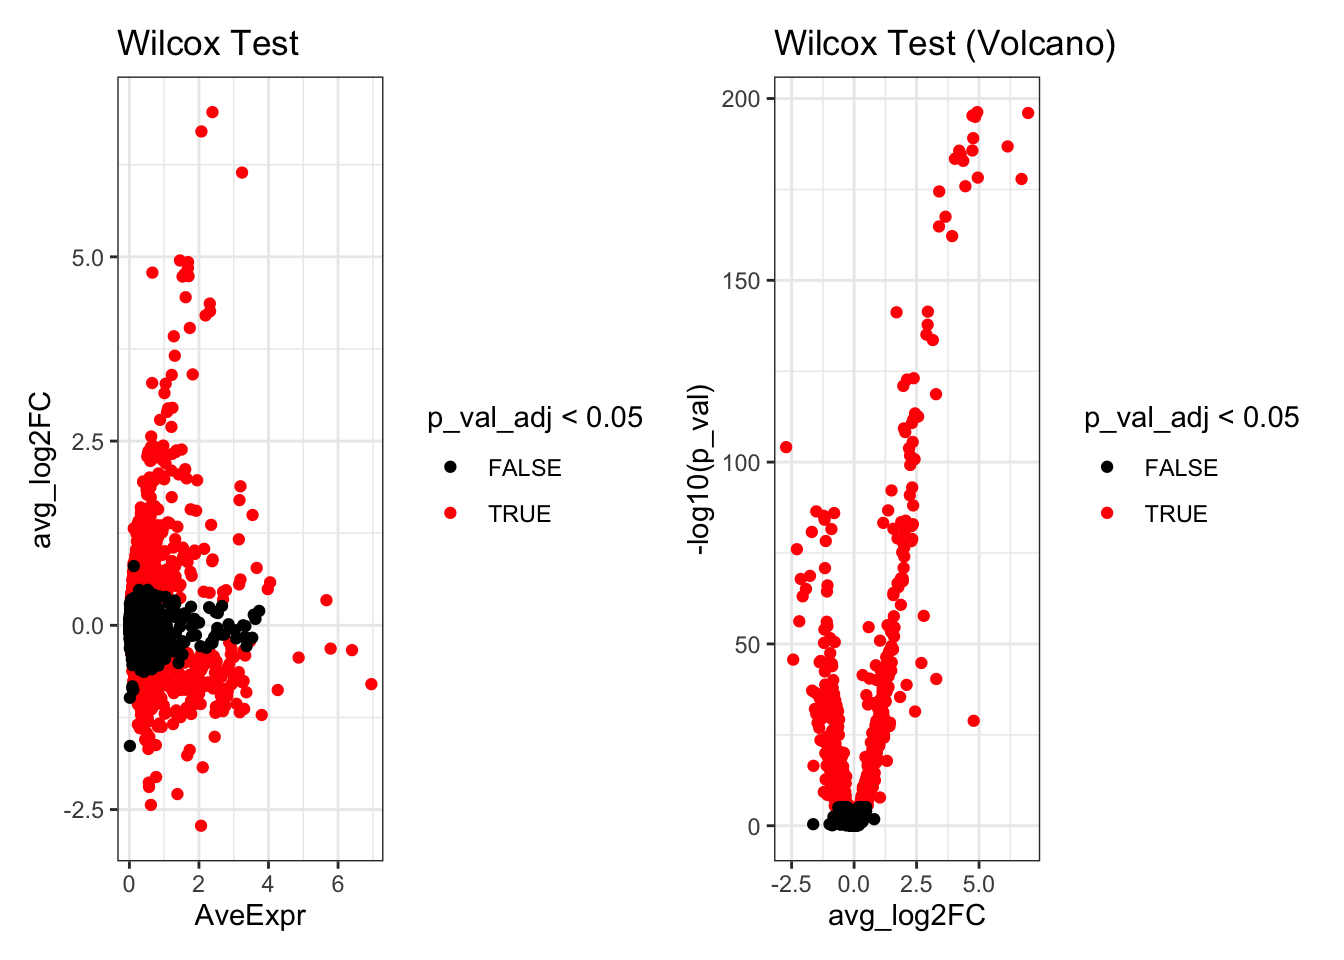
\includegraphics{scRNAseqInR_Doco_files/figure-latex/unnamed-chunk-52-1.pdf}

\hypertarget{seurat-negative-binomial}{%
\section{Seurat Negative binomial}\label{seurat-negative-binomial}}

Negative binonial test is run almost the same way - just need to specify it under `test.use'

\begin{Shaded}
\begin{Highlighting}[]

\CommentTok{\# Change Ident to Condition}
\FunctionTok{Idents}\NormalTok{(kang.celltype) }\OtherTok{\textless{}{-}}\NormalTok{ kang.celltype}\SpecialCharTok{$}\NormalTok{stim}

\CommentTok{\# default, wilcox test}
\NormalTok{de\_result\_negbinom }\OtherTok{\textless{}{-}} \FunctionTok{FindMarkers}\NormalTok{(kang.celltype, }
            \AttributeTok{test.use=}\StringTok{"negbinom"}\NormalTok{, }\CommentTok{\# Choose a different test.}
            \AttributeTok{ident.1 =} \StringTok{\textquotesingle{}stim\textquotesingle{}}\NormalTok{,}
            \AttributeTok{ident.2 =} \StringTok{\textquotesingle{}ctrl\textquotesingle{}}\NormalTok{,}
            \AttributeTok{logfc.threshold =} \DecValTok{0}\NormalTok{, }\CommentTok{\# Give me ALL results}
            \AttributeTok{min.pct =} \DecValTok{0}
\NormalTok{)}

\CommentTok{\# Add average expression for plotting}
\NormalTok{de\_result\_negbinom}\SpecialCharTok{$}\NormalTok{AveExpr}\OtherTok{\textless{}{-}} \FunctionTok{rowMeans}\NormalTok{(kang.celltype[[}\StringTok{"RNA"}\NormalTok{]][}\FunctionTok{rownames}\NormalTok{(de\_result\_negbinom),])}
\end{Highlighting}
\end{Shaded}

Look at the top differentially expressed genes.

\begin{Shaded}
\begin{Highlighting}[]
\FunctionTok{head}\NormalTok{(de\_result\_negbinom)}
\CommentTok{\#\textgreater{}        p\_val avg\_log2FC pct.1 pct.2 p\_val\_adj  AveExpr}
\CommentTok{\#\textgreater{} ISG15      0   5.787224 0.998 0.320         0 3.239774}
\CommentTok{\#\textgreater{} IFI6       0   2.578840 0.979 0.253         0 1.820140}
\CommentTok{\#\textgreater{} CXCL10     0   5.750807 0.973 0.038         0 2.388462}
\CommentTok{\#\textgreater{} LY6E       0   2.900314 0.973 0.133         0 1.736931}
\CommentTok{\#\textgreater{} IFITM3     0   3.401677 0.994 0.267         0 2.190185}
\CommentTok{\#\textgreater{} ISG20      0   3.659844 0.994 0.272         0 2.319655}
\end{Highlighting}
\end{Shaded}

\begin{Shaded}
\begin{Highlighting}[]
\NormalTok{p1 }\OtherTok{\textless{}{-}} \FunctionTok{ggplot}\NormalTok{(de\_result\_negbinom, }\FunctionTok{aes}\NormalTok{(}\AttributeTok{x=}\NormalTok{AveExpr, }\AttributeTok{y=}\NormalTok{avg\_log2FC, }\AttributeTok{col=}\NormalTok{p\_val\_adj }\SpecialCharTok{\textless{}} \FloatTok{0.05}\NormalTok{)) }\SpecialCharTok{+}
  \FunctionTok{geom\_point}\NormalTok{() }\SpecialCharTok{+}
  \FunctionTok{scale\_colour\_manual}\NormalTok{(}\AttributeTok{values=}\FunctionTok{c}\NormalTok{(}\StringTok{\textquotesingle{}TRUE\textquotesingle{}}\OtherTok{=}\StringTok{"red"}\NormalTok{,}\StringTok{\textquotesingle{}FALSE\textquotesingle{}}\OtherTok{=}\StringTok{"black"}\NormalTok{)) }\SpecialCharTok{+} 
  \FunctionTok{theme\_bw}\NormalTok{() }\SpecialCharTok{+}
  \FunctionTok{ggtitle}\NormalTok{(}\StringTok{"Negative Bionomial Test"}\NormalTok{)}


\NormalTok{p2 }\OtherTok{\textless{}{-}} \FunctionTok{ggplot}\NormalTok{(de\_result\_negbinom, }\FunctionTok{aes}\NormalTok{(}\AttributeTok{x=}\NormalTok{avg\_log2FC, }\AttributeTok{y=}\SpecialCharTok{{-}}\FunctionTok{log10}\NormalTok{(p\_val), }\AttributeTok{col=}\NormalTok{p\_val\_adj }\SpecialCharTok{\textless{}} \FloatTok{0.05}\NormalTok{)) }\SpecialCharTok{+}
  \FunctionTok{geom\_point}\NormalTok{() }\SpecialCharTok{+}
  \FunctionTok{scale\_colour\_manual}\NormalTok{(}\AttributeTok{values=}\FunctionTok{c}\NormalTok{(}\StringTok{\textquotesingle{}TRUE\textquotesingle{}}\OtherTok{=}\StringTok{"red"}\NormalTok{,}\StringTok{\textquotesingle{}FALSE\textquotesingle{}}\OtherTok{=}\StringTok{"black"}\NormalTok{)) }\SpecialCharTok{+} 
  \FunctionTok{theme\_bw}\NormalTok{() }\SpecialCharTok{+}
  \FunctionTok{ggtitle}\NormalTok{(}\StringTok{"Negative Bionomial Test (Volcano)"}\NormalTok{)}

\NormalTok{p1 }\SpecialCharTok{+}\NormalTok{ p2}
\end{Highlighting}
\end{Shaded}

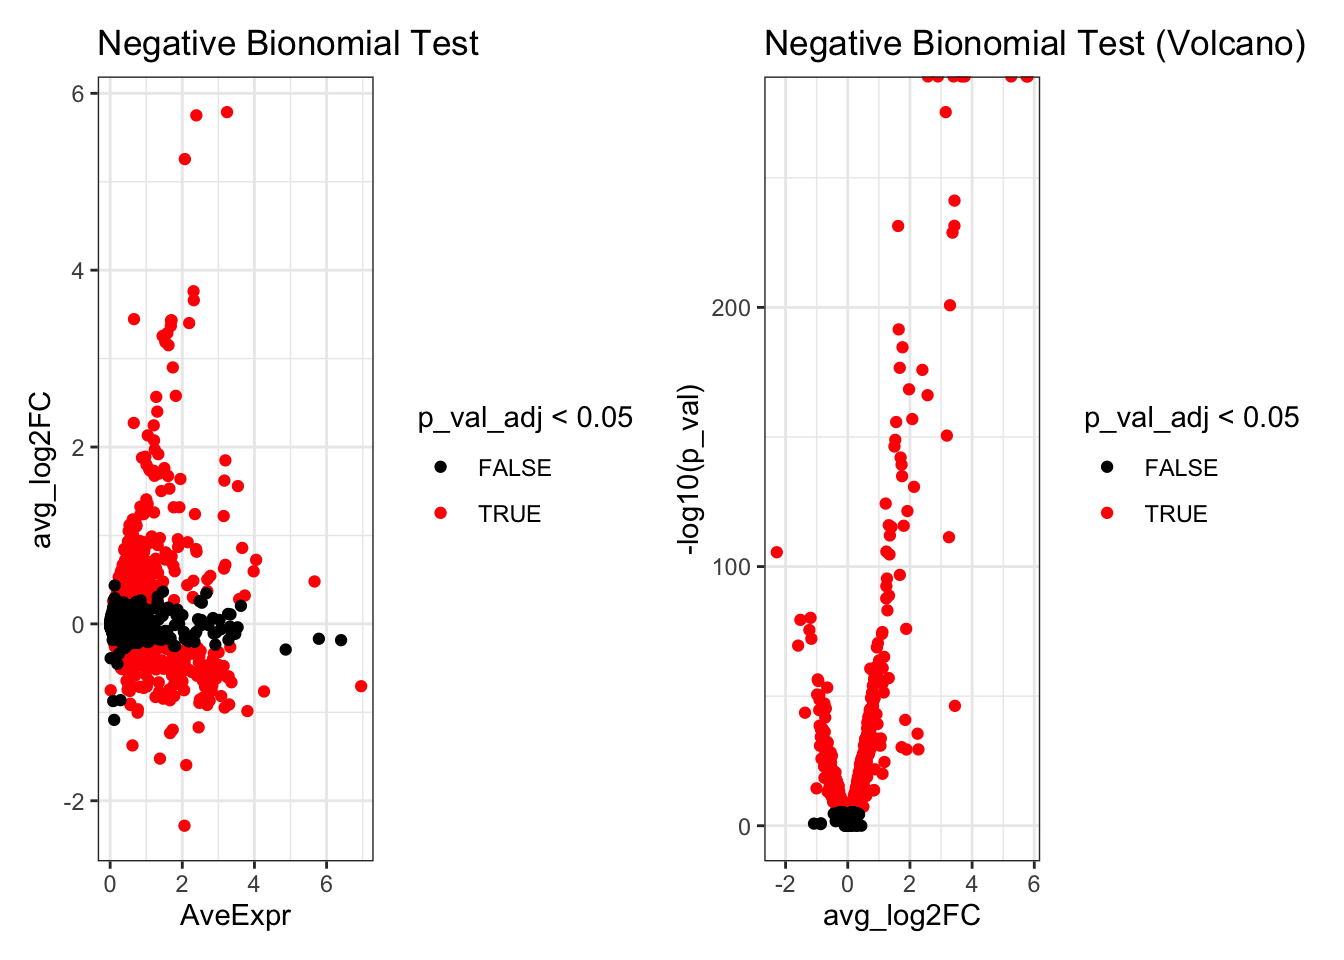
\includegraphics{scRNAseqInR_Doco_files/figure-latex/unnamed-chunk-55-1.pdf}

\hypertarget{pseudobulk}{%
\section{Pseudobulk}\label{pseudobulk}}

Pseudobulk analysis is an option where you have biological replicates. It is essentially pooling the individual cell counts and treating your expreiment like a bulk RNAseq.

First, you need to build a pseudobulk matrix - the \texttt{AggregateExpression()} function can do this, once you set the `Idents' of your seurat object to your grouping factor (here, thats a combination of individual+treatment called `sample', instead of the `stim' treatment column).

\begin{Shaded}
\begin{Highlighting}[]
\CommentTok{\# Tools for bulk differential expression}
\FunctionTok{library}\NormalTok{(limma)}
\CommentTok{\#\textgreater{} }
\CommentTok{\#\textgreater{} Attaching package: \textquotesingle{}limma\textquotesingle{}}
\CommentTok{\#\textgreater{} The following object is masked from \textquotesingle{}package:BiocGenerics\textquotesingle{}:}
\CommentTok{\#\textgreater{} }
\CommentTok{\#\textgreater{}     plotMA}
\FunctionTok{library}\NormalTok{(edgeR)}
\CommentTok{\#\textgreater{} }
\CommentTok{\#\textgreater{} Attaching package: \textquotesingle{}edgeR\textquotesingle{}}
\CommentTok{\#\textgreater{} The following object is masked from \textquotesingle{}package:SingleCellExperiment\textquotesingle{}:}
\CommentTok{\#\textgreater{} }
\CommentTok{\#\textgreater{}     cpm}


\CommentTok{\# Change idents to ind for grouping.}
\NormalTok{kang.celltype}\SpecialCharTok{$}\NormalTok{sample }\OtherTok{\textless{}{-}} \FunctionTok{factor}\NormalTok{(}\FunctionTok{paste}\NormalTok{(kang.celltype}\SpecialCharTok{$}\NormalTok{stim, kang.celltype}\SpecialCharTok{$}\NormalTok{ind, }\AttributeTok{sep=}\StringTok{"\_"}\NormalTok{))}
\FunctionTok{Idents}\NormalTok{(kang.celltype) }\OtherTok{\textless{}{-}}\NormalTok{ kang.celltype}\SpecialCharTok{$}\NormalTok{sample}

\CommentTok{\# THen pool together counts in those groups}
\NormalTok{pseudobulk\_matrix }\OtherTok{\textless{}{-}} \FunctionTok{AggregateExpression}\NormalTok{( kang.celltype,  }\AttributeTok{slot =} \StringTok{\textquotesingle{}counts\textquotesingle{}}\NormalTok{, }\AttributeTok{assays=}\StringTok{\textquotesingle{}RNA\textquotesingle{}}\NormalTok{ )[[}\StringTok{\textquotesingle{}RNA\textquotesingle{}}\NormalTok{]]}
\FunctionTok{colnames}\NormalTok{(pseudobulk\_matrix) }\OtherTok{\textless{}{-}} \FunctionTok{as.character}\NormalTok{(}\FunctionTok{colnames}\NormalTok{(pseudobulk\_matrix)) }\CommentTok{\# Changes colnames to simple text}
\NormalTok{pseudobulk\_matrix[}\DecValTok{1}\SpecialCharTok{:}\DecValTok{5}\NormalTok{,]}
\CommentTok{\#\textgreater{}          ctrl\_101 ctrl\_1015 ctrl\_1016 ctrl\_1039 ctrl\_107}
\CommentTok{\#\textgreater{} NOC2L           2         7         0         0        3}
\CommentTok{\#\textgreater{} HES4            0         3         2         1        0}
\CommentTok{\#\textgreater{} ISG15          31       185       236        41       26}
\CommentTok{\#\textgreater{} TNFRSF18        0         3         4         2        0}
\CommentTok{\#\textgreater{} TNFRSF4         0         2         0         0        0}
\CommentTok{\#\textgreater{}          ctrl\_1244 ctrl\_1256 ctrl\_1488 stim\_101 stim\_1015}
\CommentTok{\#\textgreater{} NOC2L            3         3         1        1         4}
\CommentTok{\#\textgreater{} HES4             0         0         1       32       161}
\CommentTok{\#\textgreater{} ISG15           20       125        10     5239     19539}
\CommentTok{\#\textgreater{} TNFRSF18         0         3         4        1         1}
\CommentTok{\#\textgreater{} TNFRSF4          1         0         2        2         0}
\CommentTok{\#\textgreater{}          stim\_1016 stim\_1039 stim\_107 stim\_1244 stim\_1256}
\CommentTok{\#\textgreater{} NOC2L            1         1        4         2         1}
\CommentTok{\#\textgreater{} HES4            40        40       54        74        89}
\CommentTok{\#\textgreater{} ISG15         5556      3135     5012      8114      8277}
\CommentTok{\#\textgreater{} TNFRSF18         0         0        1         1         0}
\CommentTok{\#\textgreater{} TNFRSF4          2         0        0         1         2}
\CommentTok{\#\textgreater{}          stim\_1488}
\CommentTok{\#\textgreater{} NOC2L            0}
\CommentTok{\#\textgreater{} HES4            78}
\CommentTok{\#\textgreater{} ISG15         6401}
\CommentTok{\#\textgreater{} TNFRSF18         0}
\CommentTok{\#\textgreater{} TNFRSF4          0}
\end{Highlighting}
\end{Shaded}

Now it looks like a bulk RNAseq experiment, so treat it like one.

\begin{Shaded}
\begin{Highlighting}[]
\NormalTok{dge }\OtherTok{\textless{}{-}} \FunctionTok{DGEList}\NormalTok{(pseudobulk\_matrix)}
\NormalTok{dge }\OtherTok{\textless{}{-}} \FunctionTok{calcNormFactors}\NormalTok{(dge)}

\NormalTok{stim }\OtherTok{\textless{}{-}} \FunctionTok{gsub}\NormalTok{(}\StringTok{"\_.*"}\NormalTok{,}\StringTok{""}\NormalTok{,}\FunctionTok{colnames}\NormalTok{(pseudobulk\_matrix))}
\NormalTok{ind  }\OtherTok{\textless{}{-}} \FunctionTok{as.character}\NormalTok{(}\FunctionTok{gsub}\NormalTok{(}\StringTok{".*\_"}\NormalTok{,}\StringTok{""}\NormalTok{,}\FunctionTok{colnames}\NormalTok{(pseudobulk\_matrix))) }\CommentTok{\# ind should be treated as text, not a number!}

\NormalTok{design }\OtherTok{\textless{}{-}} \FunctionTok{model.matrix}\NormalTok{( }\SpecialCharTok{\textasciitilde{}}\DecValTok{0} \SpecialCharTok{+}\NormalTok{ stim }\SpecialCharTok{+}\NormalTok{ ind)}
\NormalTok{vm  }\OtherTok{\textless{}{-}} \FunctionTok{voom}\NormalTok{(dge, }\AttributeTok{design =}\NormalTok{ design, }\AttributeTok{plot =} \ConstantTok{FALSE}\NormalTok{)}
\NormalTok{fit }\OtherTok{\textless{}{-}} \FunctionTok{lmFit}\NormalTok{(vm, }\AttributeTok{design =}\NormalTok{ design)}

\NormalTok{contrasts }\OtherTok{\textless{}{-}} \FunctionTok{makeContrasts}\NormalTok{(stimstim }\SpecialCharTok{{-}}\NormalTok{ stimctrl, }\AttributeTok{levels=}\FunctionTok{coef}\NormalTok{(fit))}
\NormalTok{fit }\OtherTok{\textless{}{-}} \FunctionTok{contrasts.fit}\NormalTok{(fit, contrasts)}
\NormalTok{fit }\OtherTok{\textless{}{-}} \FunctionTok{eBayes}\NormalTok{(fit)}

\NormalTok{de\_result\_pseudobulk }\OtherTok{\textless{}{-}} \FunctionTok{topTable}\NormalTok{(fit, }\AttributeTok{n =} \ConstantTok{Inf}\NormalTok{, }\AttributeTok{adjust.method =} \StringTok{"BH"}\NormalTok{)}
\NormalTok{de\_result\_pseudobulk }\OtherTok{\textless{}{-}} \FunctionTok{arrange}\NormalTok{(de\_result\_pseudobulk , adj.P.Val)}
\end{Highlighting}
\end{Shaded}

Look at the significantly differentially expressed genes:

\begin{Shaded}
\begin{Highlighting}[]
\FunctionTok{head}\NormalTok{(de\_result\_pseudobulk)}
\CommentTok{\#\textgreater{}           logFC   AveExpr        t      P.Value}
\CommentTok{\#\textgreater{} ISG20  5.151090 10.311187 34.62460 1.377577e{-}28}
\CommentTok{\#\textgreater{} ISG15  6.926462 11.895928 33.45672 4.402969e{-}28}
\CommentTok{\#\textgreater{} CXCL11 9.051653  7.260525 32.07090 1.838679e{-}27}
\CommentTok{\#\textgreater{} IFIT3  6.980913  8.420719 28.54319 9.234346e{-}26}
\CommentTok{\#\textgreater{} HERC5  6.998957  5.602349 28.68162 7.853707e{-}26}
\CommentTok{\#\textgreater{} TMSB10 1.959063 11.466981 27.48469 3.264041e{-}25}
\CommentTok{\#\textgreater{}           adj.P.Val        B}
\CommentTok{\#\textgreater{} ISG20  9.940598e{-}25 55.27733}
\CommentTok{\#\textgreater{} ISG15  1.588591e{-}24 54.12183}
\CommentTok{\#\textgreater{} CXCL11 4.422636e{-}24 51.56638}
\CommentTok{\#\textgreater{} IFIT3  1.332701e{-}22 48.32088}
\CommentTok{\#\textgreater{} HERC5  1.332701e{-}22 48.02111}
\CommentTok{\#\textgreater{} TMSB10 2.950103e{-}22 47.34483}
\end{Highlighting}
\end{Shaded}

\begin{Shaded}
\begin{Highlighting}[]
\NormalTok{p1 }\OtherTok{\textless{}{-}} \FunctionTok{ggplot}\NormalTok{(de\_result\_pseudobulk, }\FunctionTok{aes}\NormalTok{(}\AttributeTok{x=}\NormalTok{AveExpr, }\AttributeTok{y=}\NormalTok{logFC, }\AttributeTok{col=}\NormalTok{adj.P.Val }\SpecialCharTok{\textless{}} \FloatTok{0.05}\NormalTok{)) }\SpecialCharTok{+}
  \FunctionTok{geom\_point}\NormalTok{() }\SpecialCharTok{+}
  \FunctionTok{scale\_colour\_manual}\NormalTok{(}\AttributeTok{values=}\FunctionTok{c}\NormalTok{(}\StringTok{\textquotesingle{}TRUE\textquotesingle{}}\OtherTok{=}\StringTok{"red"}\NormalTok{,}\StringTok{\textquotesingle{}FALSE\textquotesingle{}}\OtherTok{=}\StringTok{"black"}\NormalTok{)) }\SpecialCharTok{+} 
  \FunctionTok{theme\_bw}\NormalTok{() }\SpecialCharTok{+}
  \FunctionTok{ggtitle}\NormalTok{(}\StringTok{"Pseudobulk"}\NormalTok{)}


\NormalTok{p2 }\OtherTok{\textless{}{-}} \FunctionTok{ggplot}\NormalTok{(de\_result\_pseudobulk, }\FunctionTok{aes}\NormalTok{(}\AttributeTok{x=}\NormalTok{logFC, }\AttributeTok{y=}\SpecialCharTok{{-}}\FunctionTok{log10}\NormalTok{(P.Value), }\AttributeTok{col=}\NormalTok{adj.P.Val }\SpecialCharTok{\textless{}} \FloatTok{0.05}\NormalTok{)) }\SpecialCharTok{+}
  \FunctionTok{geom\_point}\NormalTok{() }\SpecialCharTok{+}
  \FunctionTok{scale\_colour\_manual}\NormalTok{(}\AttributeTok{values=}\FunctionTok{c}\NormalTok{(}\StringTok{\textquotesingle{}TRUE\textquotesingle{}}\OtherTok{=}\StringTok{"red"}\NormalTok{,}\StringTok{\textquotesingle{}FALSE\textquotesingle{}}\OtherTok{=}\StringTok{"black"}\NormalTok{)) }\SpecialCharTok{+} 
  \FunctionTok{theme\_bw}\NormalTok{() }\SpecialCharTok{+}
  \FunctionTok{ggtitle}\NormalTok{(}\StringTok{"Pseudobulk Test (Volcano)"}\NormalTok{)}

\NormalTok{p1 }\SpecialCharTok{+}\NormalTok{ p2}
\end{Highlighting}
\end{Shaded}

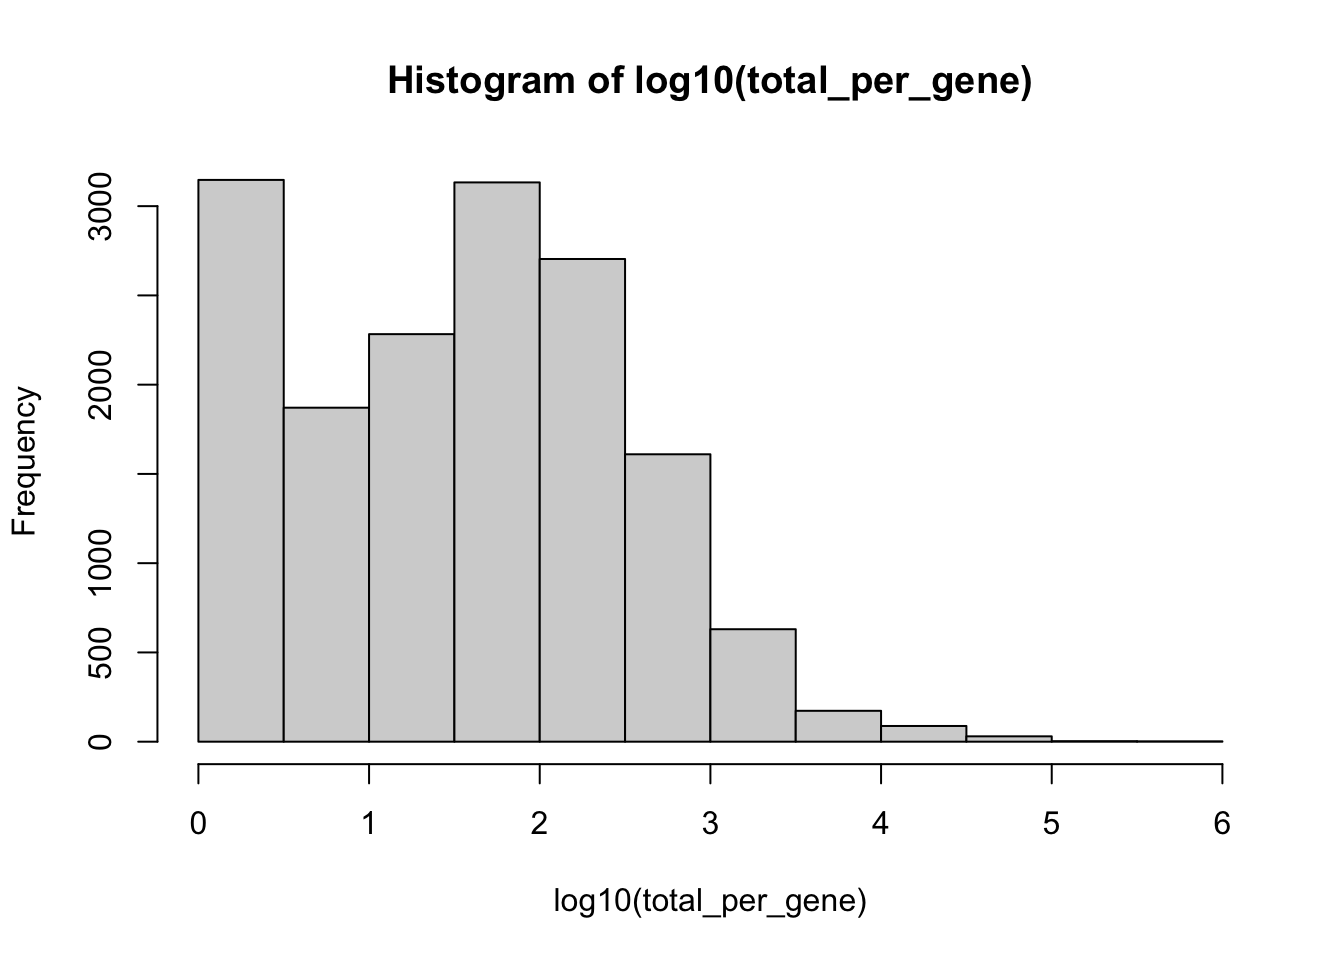
\includegraphics{scRNAseqInR_Doco_files/figure-latex/unnamed-chunk-59-1.pdf}

\hypertarget{challenge-what-method}{%
\subsubsection*{Challenge: What method?}\label{challenge-what-method}}
\addcontentsline{toc}{subsubsection}{Challenge: What method?}

These methods give different results. How could and decide which to use? How could you check an individual gene?

\hypertarget{CellCycle}{%
\chapter{Cell cycle Assignment}\label{CellCycle}}

In some datasets, the phase of cell cycle that a cell is in (G1/G2M/S) can account for
alot of the observed transcriptomic variation. There may be clustering by phase, or
separation in the UMAP by phase.

Seurat provides a simple method for assigning cell cycle state to each cell. Other methods are available.

More information about assigning cell cycle states to cells is in the \href{https://satijalab.org/seurat/articles/cell_cycle_vignette.html}{cell cycle vignette}

\begin{Shaded}
\begin{Highlighting}[]
\CommentTok{\# A list of cell cycle markers, from Tirosh et al, 2015, is loaded with Seurat.  We can}
\CommentTok{\# segregate this list into markers of G2/M phase and markers of S phase}
\NormalTok{s.genes   }\OtherTok{\textless{}{-}}\NormalTok{ cc.genes}\SpecialCharTok{$}\NormalTok{s.genes}
\NormalTok{g2m.genes }\OtherTok{\textless{}{-}}\NormalTok{ cc.genes}\SpecialCharTok{$}\NormalTok{g2m.genes}

\CommentTok{\# Use those lists with the cell cycle scoring function in Seurat.}
\NormalTok{pbmc }\OtherTok{\textless{}{-}} \FunctionTok{CellCycleScoring}\NormalTok{(pbmc, }\AttributeTok{s.features =}\NormalTok{ s.genes, }\AttributeTok{g2m.features =}\NormalTok{ g2m.genes)}
\CommentTok{\#\textgreater{} Warning: The following features are not present in the}
\CommentTok{\#\textgreater{} object: DTL, UHRF1, MLF1IP, EXO1, CASP8AP2, BRIP1, E2F8,}
\CommentTok{\#\textgreater{} not searching for symbol synonyms}
\CommentTok{\#\textgreater{} Warning: The following features are not present in the}
\CommentTok{\#\textgreater{} object: FAM64A, BUB1, HJURP, CDCA3, TTK, CDC25C, DLGAP5,}
\CommentTok{\#\textgreater{} CDCA2, ANLN, GAS2L3, not searching for symbol synonyms}
\end{Highlighting}
\end{Shaded}

Which adds S.Score, G2M.Score and Phase calls to the metadata.

\begin{Shaded}
\begin{Highlighting}[]
\FunctionTok{head}\NormalTok{(pbmc}\SpecialCharTok{@}\NormalTok{meta.data)}
\CommentTok{\#\textgreater{}                  orig.ident nCount\_RNA nFeature\_RNA}
\CommentTok{\#\textgreater{} AAACATACAACCAC{-}1     pbmc3k       2419          779}
\CommentTok{\#\textgreater{} AAACATTGAGCTAC{-}1     pbmc3k       4903         1352}
\CommentTok{\#\textgreater{} AAACATTGATCAGC{-}1     pbmc3k       3147         1129}
\CommentTok{\#\textgreater{} AAACCGTGCTTCCG{-}1     pbmc3k       2639          960}
\CommentTok{\#\textgreater{} AAACCGTGTATGCG{-}1     pbmc3k        980          521}
\CommentTok{\#\textgreater{} AAACGCACTGGTAC{-}1     pbmc3k       2163          781}
\CommentTok{\#\textgreater{}                  percent.mt RNA\_snn\_res.0.5 seurat\_clusters}
\CommentTok{\#\textgreater{} AAACATACAACCAC{-}1  3.0177759               2               6}
\CommentTok{\#\textgreater{} AAACATTGAGCTAC{-}1  3.7935958               3               1}
\CommentTok{\#\textgreater{} AAACATTGATCAGC{-}1  0.8897363               2               0}
\CommentTok{\#\textgreater{} AAACCGTGCTTCCG{-}1  1.7430845               1               5}
\CommentTok{\#\textgreater{} AAACCGTGTATGCG{-}1  1.2244898               6               8}
\CommentTok{\#\textgreater{} AAACGCACTGGTAC{-}1  1.6643551               2               0}
\CommentTok{\#\textgreater{}                  RNA\_snn\_res.0.1 RNA\_snn\_res.0.2}
\CommentTok{\#\textgreater{} AAACATACAACCAC{-}1               0               0}
\CommentTok{\#\textgreater{} AAACATTGAGCTAC{-}1               3               3}
\CommentTok{\#\textgreater{} AAACATTGATCAGC{-}1               0               0}
\CommentTok{\#\textgreater{} AAACCGTGCTTCCG{-}1               1               1}
\CommentTok{\#\textgreater{} AAACCGTGTATGCG{-}1               2               2}
\CommentTok{\#\textgreater{} AAACGCACTGGTAC{-}1               0               0}
\CommentTok{\#\textgreater{}                  RNA\_snn\_res.0.3 RNA\_snn\_res.0.4}
\CommentTok{\#\textgreater{} AAACATACAACCAC{-}1               0               2}
\CommentTok{\#\textgreater{} AAACATTGAGCTAC{-}1               3               3}
\CommentTok{\#\textgreater{} AAACATTGATCAGC{-}1               0               2}
\CommentTok{\#\textgreater{} AAACCGTGCTTCCG{-}1               1               1}
\CommentTok{\#\textgreater{} AAACCGTGTATGCG{-}1               2               6}
\CommentTok{\#\textgreater{} AAACGCACTGGTAC{-}1               0               2}
\CommentTok{\#\textgreater{}                  RNA\_snn\_res.0.6 RNA\_snn\_res.0.7}
\CommentTok{\#\textgreater{} AAACATACAACCAC{-}1               1               1}
\CommentTok{\#\textgreater{} AAACATTGAGCTAC{-}1               3               3}
\CommentTok{\#\textgreater{} AAACATTGATCAGC{-}1               1               1}
\CommentTok{\#\textgreater{} AAACCGTGCTTCCG{-}1               2               2}
\CommentTok{\#\textgreater{} AAACCGTGTATGCG{-}1               6               6}
\CommentTok{\#\textgreater{} AAACGCACTGGTAC{-}1               1               1}
\CommentTok{\#\textgreater{}                  RNA\_snn\_res.0.8 RNA\_snn\_res.0.9}
\CommentTok{\#\textgreater{} AAACATACAACCAC{-}1               6               1}
\CommentTok{\#\textgreater{} AAACATTGAGCTAC{-}1               2               2}
\CommentTok{\#\textgreater{} AAACATTGATCAGC{-}1               1               1}
\CommentTok{\#\textgreater{} AAACCGTGCTTCCG{-}1               4               4}
\CommentTok{\#\textgreater{} AAACCGTGTATGCG{-}1               8               7}
\CommentTok{\#\textgreater{} AAACGCACTGGTAC{-}1               1               1}
\CommentTok{\#\textgreater{}                  RNA\_snn\_res.1 RNA\_snn\_res.1.1}
\CommentTok{\#\textgreater{} AAACATACAACCAC{-}1             6               6}
\CommentTok{\#\textgreater{} AAACATTGAGCTAC{-}1             2               2}
\CommentTok{\#\textgreater{} AAACATTGATCAGC{-}1             1               1}
\CommentTok{\#\textgreater{} AAACCGTGCTTCCG{-}1             4               4}
\CommentTok{\#\textgreater{} AAACCGTGTATGCG{-}1             8               8}
\CommentTok{\#\textgreater{} AAACGCACTGGTAC{-}1             1               1}
\CommentTok{\#\textgreater{}                  RNA\_snn\_res.1.2 RNA\_snn\_res.1.3}
\CommentTok{\#\textgreater{} AAACATACAACCAC{-}1               6               8}
\CommentTok{\#\textgreater{} AAACATTGAGCTAC{-}1               2               2}
\CommentTok{\#\textgreater{} AAACATTGATCAGC{-}1               1               0}
\CommentTok{\#\textgreater{} AAACCGTGCTTCCG{-}1               4               5}
\CommentTok{\#\textgreater{} AAACCGTGTATGCG{-}1               8               9}
\CommentTok{\#\textgreater{} AAACGCACTGGTAC{-}1               1               0}
\CommentTok{\#\textgreater{}                  RNA\_snn\_res.1.4 RNA\_snn\_res.1.5}
\CommentTok{\#\textgreater{} AAACATACAACCAC{-}1               8               9}
\CommentTok{\#\textgreater{} AAACATTGAGCTAC{-}1               2               2}
\CommentTok{\#\textgreater{} AAACATTGATCAGC{-}1               0               1}
\CommentTok{\#\textgreater{} AAACCGTGCTTCCG{-}1               5               4}
\CommentTok{\#\textgreater{} AAACCGTGTATGCG{-}1               9               8}
\CommentTok{\#\textgreater{} AAACGCACTGGTAC{-}1               0               1}
\CommentTok{\#\textgreater{}                  RNA\_snn\_res.1.6 RNA\_snn\_res.1.7}
\CommentTok{\#\textgreater{} AAACATACAACCAC{-}1               8               8}
\CommentTok{\#\textgreater{} AAACATTGAGCTAC{-}1               1               1}
\CommentTok{\#\textgreater{} AAACATTGATCAGC{-}1               0               0}
\CommentTok{\#\textgreater{} AAACCGTGCTTCCG{-}1               3               3}
\CommentTok{\#\textgreater{} AAACCGTGTATGCG{-}1               7               7}
\CommentTok{\#\textgreater{} AAACGCACTGGTAC{-}1               0               0}
\CommentTok{\#\textgreater{}                  RNA\_snn\_res.1.8 RNA\_snn\_res.1.9}
\CommentTok{\#\textgreater{} AAACATACAACCAC{-}1               7               6}
\CommentTok{\#\textgreater{} AAACATTGAGCTAC{-}1               1               1}
\CommentTok{\#\textgreater{} AAACATTGATCAGC{-}1               0               0}
\CommentTok{\#\textgreater{} AAACCGTGCTTCCG{-}1               3               3}
\CommentTok{\#\textgreater{} AAACCGTGTATGCG{-}1               8               8}
\CommentTok{\#\textgreater{} AAACGCACTGGTAC{-}1               0               0}
\CommentTok{\#\textgreater{}                  RNA\_snn\_res.2 Naive\_CD4\_T1  cell\_label}
\CommentTok{\#\textgreater{} AAACATACAACCAC{-}1             6   1.22824523 Naive\_CD4\_T}
\CommentTok{\#\textgreater{} AAACATTGAGCTAC{-}1             1  {-}0.08111043        \textless{}NA\textgreater{}}
\CommentTok{\#\textgreater{} AAACATTGATCAGC{-}1             0  {-}0.37682601        \textless{}NA\textgreater{}}
\CommentTok{\#\textgreater{} AAACCGTGCTTCCG{-}1             5  {-}0.72739714        \textless{}NA\textgreater{}}
\CommentTok{\#\textgreater{} AAACCGTGTATGCG{-}1             8  {-}1.17396454        \textless{}NA\textgreater{}}
\CommentTok{\#\textgreater{} AAACGCACTGGTAC{-}1             0  {-}0.63807586        \textless{}NA\textgreater{}}
\CommentTok{\#\textgreater{}                  SingleR.labels     S.Score    G2M.Score}
\CommentTok{\#\textgreater{} AAACATACAACCAC{-}1        T\_cells  0.09853841 {-}0.044716507}
\CommentTok{\#\textgreater{} AAACATTGAGCTAC{-}1         B\_cell {-}0.02364305 {-}0.046889929}
\CommentTok{\#\textgreater{} AAACATTGATCAGC{-}1        T\_cells {-}0.02177266  0.074841537}
\CommentTok{\#\textgreater{} AAACCGTGCTTCCG{-}1       Monocyte  0.03794398  0.006575446}
\CommentTok{\#\textgreater{} AAACCGTGTATGCG{-}1        NK\_cell {-}0.03309970  0.027910063}
\CommentTok{\#\textgreater{} AAACGCACTGGTAC{-}1        T\_cells {-}0.04814181 {-}0.078164839}
\CommentTok{\#\textgreater{}                  Phase}
\CommentTok{\#\textgreater{} AAACATACAACCAC{-}1     S}
\CommentTok{\#\textgreater{} AAACATTGAGCTAC{-}1    G1}
\CommentTok{\#\textgreater{} AAACATTGATCAGC{-}1   G2M}
\CommentTok{\#\textgreater{} AAACCGTGCTTCCG{-}1     S}
\CommentTok{\#\textgreater{} AAACCGTGTATGCG{-}1   G2M}
\CommentTok{\#\textgreater{} AAACGCACTGGTAC{-}1    G1}
\end{Highlighting}
\end{Shaded}

We can then check the cell phase on the UMAP. In this dataset, phase isn't driving the clustering, and would not require any further handling.

\begin{Shaded}
\begin{Highlighting}[]
\FunctionTok{DimPlot}\NormalTok{(pbmc, }\AttributeTok{reduction =} \StringTok{\textquotesingle{}umap\textquotesingle{}}\NormalTok{, }\AttributeTok{group.by =} \StringTok{"Phase"}\NormalTok{)}
\end{Highlighting}
\end{Shaded}

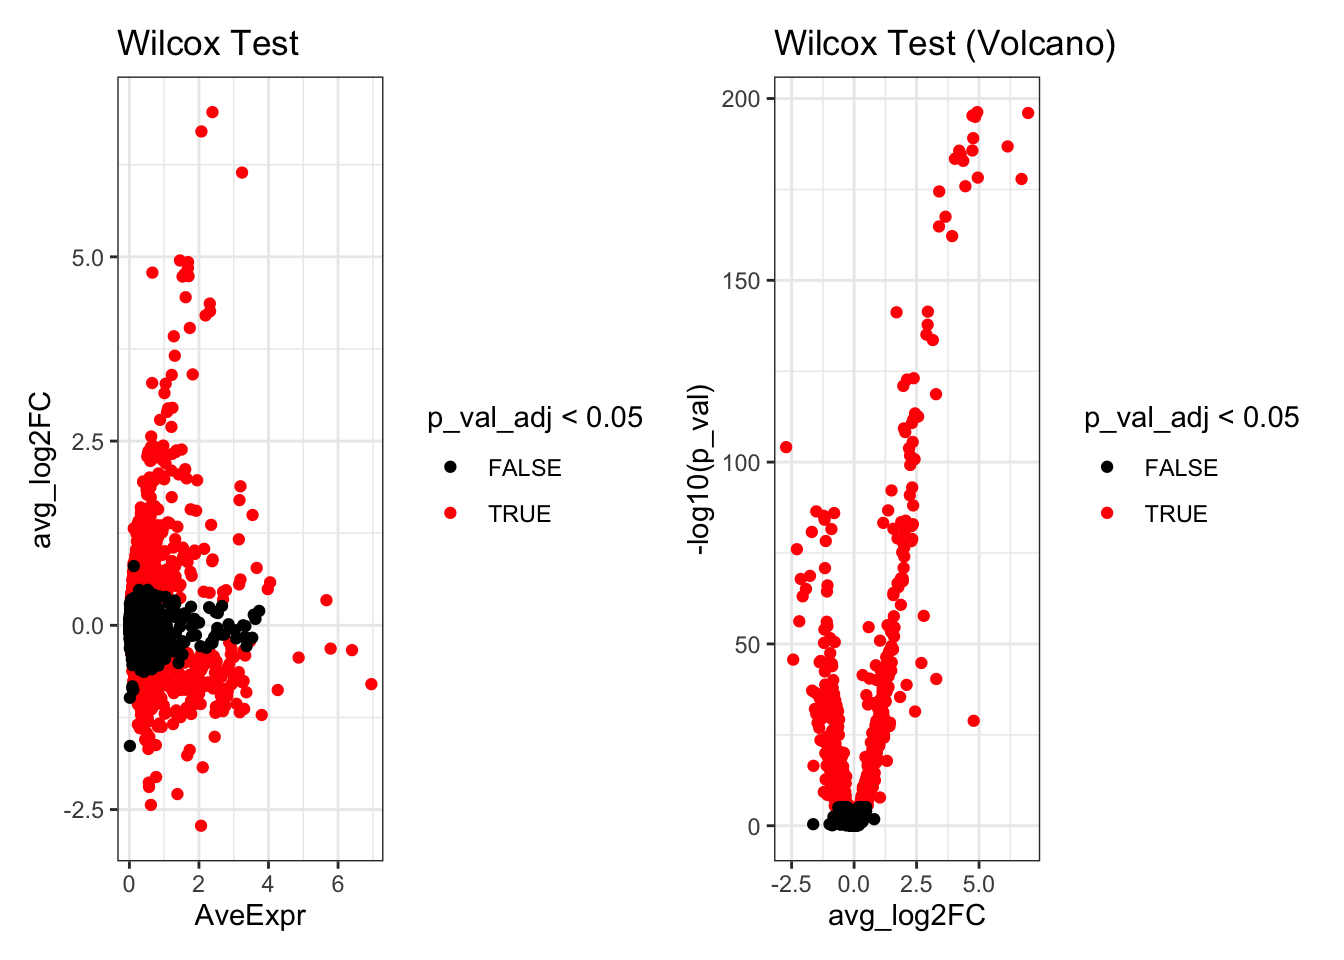
\includegraphics{scRNAseqInR_Doco_files/figure-latex/unnamed-chunk-62-1.pdf}

Where a bias \emph{is} present, your course of action depends on the task at hand. It might involve `regressing out' the cell cycle variation with ScaleData(), omitting cell-cycle dominated clusters, or just accounting for it in your differential expression calculations.

If you are working with non-human data, you will need to convert these gene lists, or find new cell cycle associated genes in your species.

\hypertarget{Harmony}{%
\chapter{Data set integration with Harmony}\label{Harmony}}

\hypertarget{why-do-we-need-to-do-this-2}{%
\subsection{Why do we need to do this?}\label{why-do-we-need-to-do-this-2}}

You can have data coming from different samples, batches or experiments and you will need to combine them.

\hypertarget{section-2}{%
\subsection{}\label{section-2}}

When data is collected from multiple samples, multiple runs of the single cell sequencing library preparation, or multiple conditions, cells of the same type may become separated in the UMAP and be put into several different clusters.

For the purpose of clustering and cell identification, we would like to remove such effects.

We will now look at \href{https://www.ncbi.nlm.nih.gov/geo/query/acc.cgi?acc=GSE96583}{GSE96583}, another PBMC dataset. For speed, we will be looking at a subset of 5000 cells from this data. The cells in this dataset were pooled from eight individual donors. A nice feature is that genetic differences allow some of the cell doublets to be identified. This data contains two batches of single cell sequencing. One of the batches was stimulated with IFN-beta.

The data has already been processed as we have done with the first PBMC dataset, and can be loaded from \texttt{kang2018.rds}.

\begin{Shaded}
\begin{Highlighting}[]
\NormalTok{kang }\OtherTok{\textless{}{-}} \FunctionTok{readRDS}\NormalTok{(}\StringTok{"data/kang2018.rds"}\NormalTok{)}

\FunctionTok{head}\NormalTok{(kang}\SpecialCharTok{@}\NormalTok{meta.data)}
\CommentTok{\#\textgreater{}                     orig.ident nCount\_RNA nFeature\_RNA  ind}
\CommentTok{\#\textgreater{} AGGGCGCTATTTCC{-}1 SeuratProject       2020          523 1256}
\CommentTok{\#\textgreater{} GGAGACGATTCGTT{-}1 SeuratProject        840          381 1256}
\CommentTok{\#\textgreater{} CACCGTTGTCGTAG{-}1 SeuratProject       3097          995 1016}
\CommentTok{\#\textgreater{} TATCGTACACGCAT{-}1 SeuratProject       1011          540 1488}
\CommentTok{\#\textgreater{} TGACGCCTTGCTTT{-}1 SeuratProject        570          367  101}
\CommentTok{\#\textgreater{} TACGAGACCTATTC{-}1 SeuratProject       2399          770 1244}
\CommentTok{\#\textgreater{}                  stim              cell multiplets}
\CommentTok{\#\textgreater{} AGGGCGCTATTTCC{-}1 stim   CD14+ Monocytes    singlet}
\CommentTok{\#\textgreater{} GGAGACGATTCGTT{-}1 stim       CD4 T cells    singlet}
\CommentTok{\#\textgreater{} CACCGTTGTCGTAG{-}1 ctrl FCGR3A+ Monocytes    singlet}
\CommentTok{\#\textgreater{} TATCGTACACGCAT{-}1 stim           B cells    singlet}
\CommentTok{\#\textgreater{} TGACGCCTTGCTTT{-}1 ctrl       CD4 T cells       ambs}
\CommentTok{\#\textgreater{} TACGAGACCTATTC{-}1 stim       CD4 T cells    singlet}
\end{Highlighting}
\end{Shaded}

\begin{itemize}
\tightlist
\item
  \texttt{ind} identifies a cell as coming from one of 8 individuals.
\item
  \texttt{stim} identifies a cell as control or stimulated with IFN-beta.
\item
  \texttt{cell} contains the cell types identified by the creators of this data set.
\item
  \texttt{multiplets} classifies cells as singlet or doublet.
\end{itemize}

\begin{Shaded}
\begin{Highlighting}[]
\FunctionTok{DimPlot}\NormalTok{(kang, }\AttributeTok{reduction=}\StringTok{"umap"}\NormalTok{, }\AttributeTok{group.by=}\StringTok{"ind"}\NormalTok{)}
\end{Highlighting}
\end{Shaded}

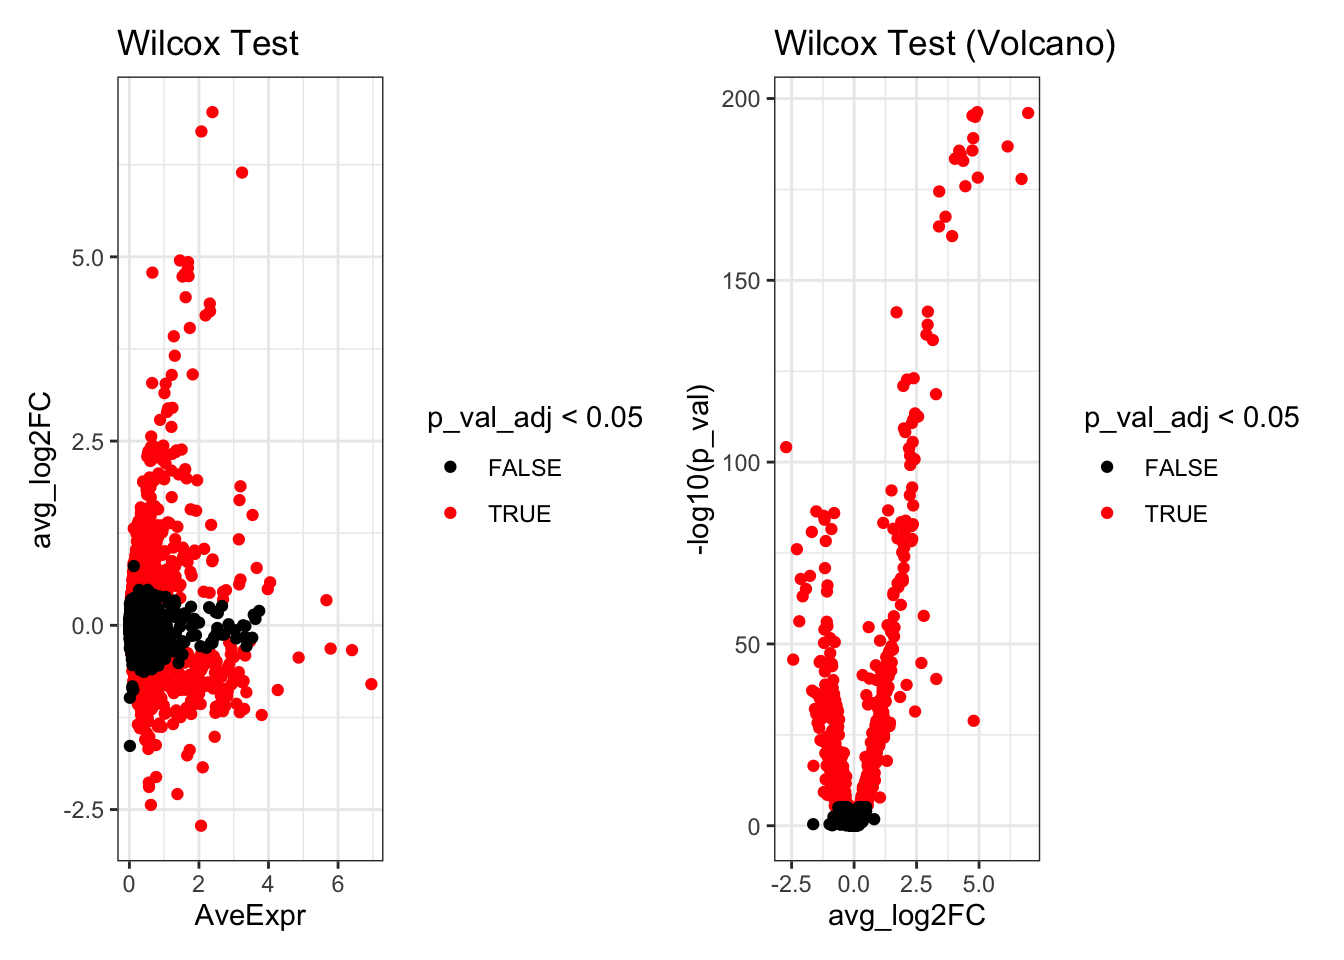
\includegraphics{scRNAseqInR_Doco_files/figure-latex/unnamed-chunk-65-1.pdf}

\begin{Shaded}
\begin{Highlighting}[]
\FunctionTok{DimPlot}\NormalTok{(kang, }\AttributeTok{reduction=}\StringTok{"umap"}\NormalTok{, }\AttributeTok{group.by=}\StringTok{"stim"}\NormalTok{)}
\end{Highlighting}
\end{Shaded}

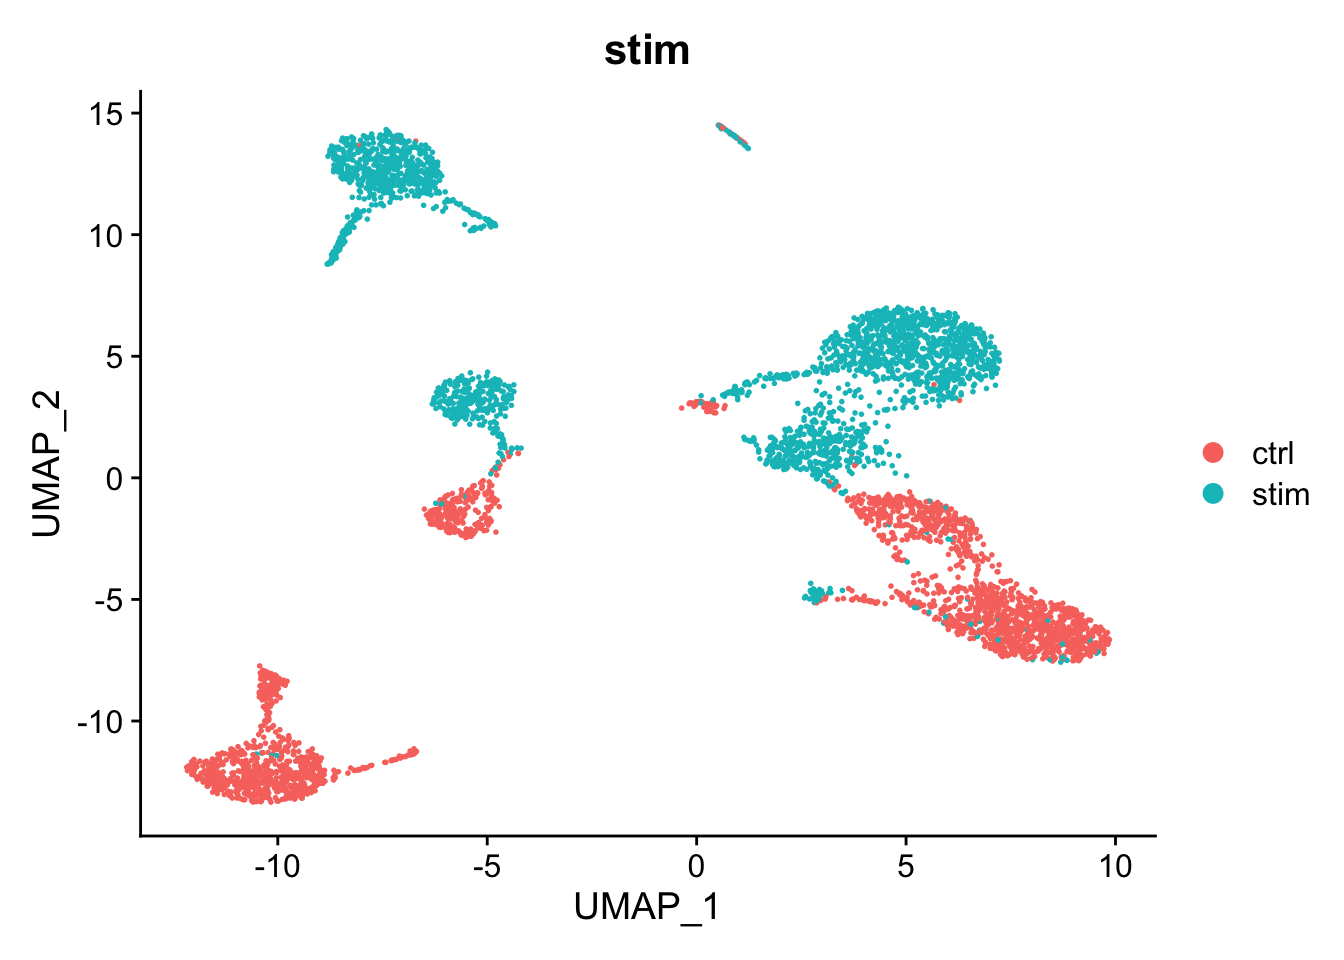
\includegraphics{scRNAseqInR_Doco_files/figure-latex/unnamed-chunk-65-2.pdf}

\begin{Shaded}
\begin{Highlighting}[]
\FunctionTok{DimPlot}\NormalTok{(kang, }\AttributeTok{reduction=}\StringTok{"pca"}\NormalTok{, }\AttributeTok{group.by=}\StringTok{"stim"}\NormalTok{)}
\end{Highlighting}
\end{Shaded}

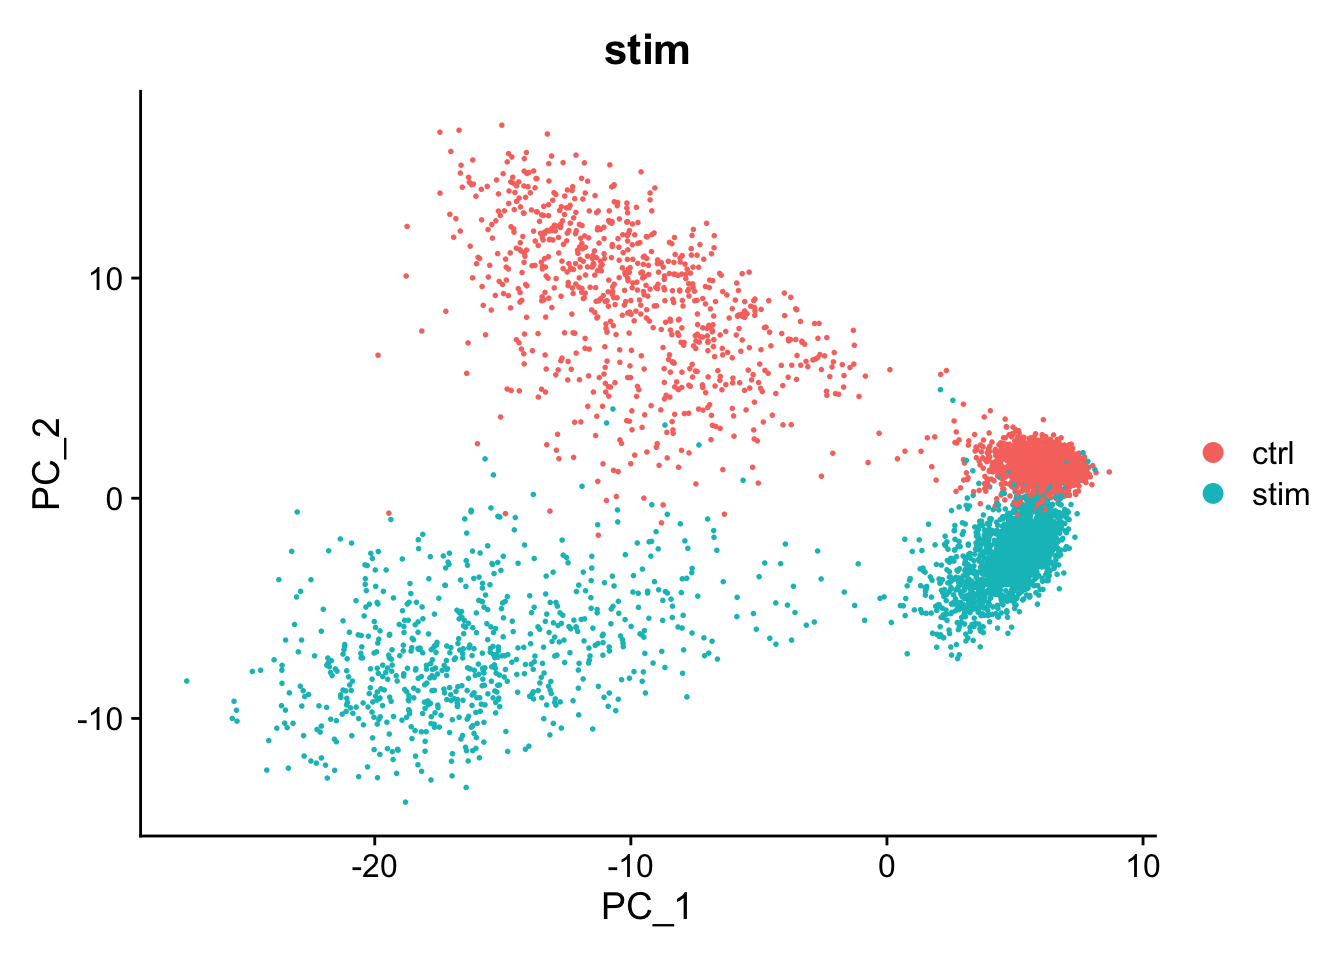
\includegraphics{scRNAseqInR_Doco_files/figure-latex/unnamed-chunk-65-3.pdf}

\begin{Shaded}
\begin{Highlighting}[]

\NormalTok{kang }\OtherTok{\textless{}{-}} \FunctionTok{FindNeighbors}\NormalTok{(kang, }\AttributeTok{reduction=}\StringTok{"pca"}\NormalTok{, }\AttributeTok{dims=}\DecValTok{1}\SpecialCharTok{:}\DecValTok{10}\NormalTok{)}
\CommentTok{\#\textgreater{} Computing nearest neighbor graph}
\CommentTok{\#\textgreater{} Computing SNN}
\NormalTok{kang }\OtherTok{\textless{}{-}} \FunctionTok{FindClusters}\NormalTok{(kang, }\AttributeTok{resolution=}\FloatTok{0.25}\NormalTok{)}
\CommentTok{\#\textgreater{} Modularity Optimizer version 1.3.0 by Ludo Waltman and Nees Jan van Eck}
\CommentTok{\#\textgreater{} }
\CommentTok{\#\textgreater{} Number of nodes: 5000}
\CommentTok{\#\textgreater{} Number of edges: 175130}
\CommentTok{\#\textgreater{} }
\CommentTok{\#\textgreater{} Running Louvain algorithm...}
\CommentTok{\#\textgreater{} Maximum modularity in 10 random starts: 0.9501}
\CommentTok{\#\textgreater{} Number of communities: 12}
\CommentTok{\#\textgreater{} Elapsed time: 0 seconds}
\NormalTok{kang}\SpecialCharTok{$}\NormalTok{pca\_clusters }\OtherTok{\textless{}{-}}\NormalTok{ kang}\SpecialCharTok{$}\NormalTok{seurat\_clusters}

\FunctionTok{DimPlot}\NormalTok{(kang, }\AttributeTok{reduction=}\StringTok{"umap"}\NormalTok{, }\AttributeTok{group.by=}\StringTok{"pca\_clusters"}\NormalTok{)}
\end{Highlighting}
\end{Shaded}

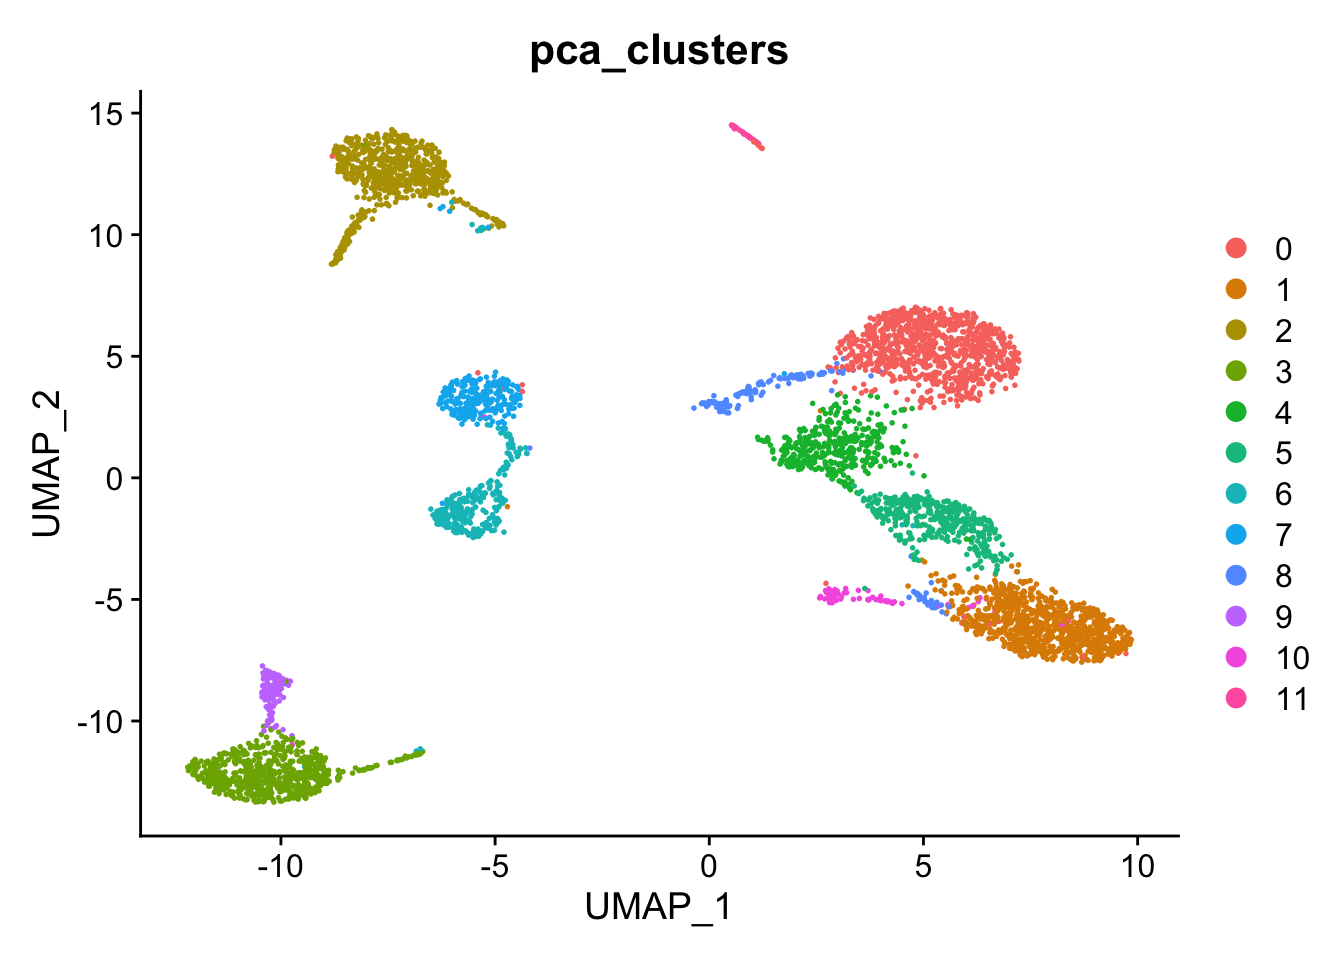
\includegraphics{scRNAseqInR_Doco_files/figure-latex/unnamed-chunk-65-4.pdf}

There is a big difference between unstimulated and stimulated cells. This has split cells of the same type into pairs of clusters. If the difference was simply uniform, we could regress it out (e.g.~using \texttt{ScaleData(...,\ vars.to.regress="stim")}). However, as can be seen in the PCA plot, the difference is not uniform and we need to do something cleverer.

We will use \href{https://github.com/immunogenomics/harmony}{Harmony}, which can remove non-uniform effects. We will try to remove both the small differences between individuals and the large difference between the unstimulated and stimulated cells.

Harmony operates only on the PCA scores. The original gene expression levels remain unaltered.

\begin{Shaded}
\begin{Highlighting}[]
\FunctionTok{library}\NormalTok{(harmony)}
\CommentTok{\#\textgreater{} Loading required package: Rcpp}

\NormalTok{kang }\OtherTok{\textless{}{-}} \FunctionTok{RunHarmony}\NormalTok{(kang, }\FunctionTok{c}\NormalTok{(}\StringTok{"stim"}\NormalTok{, }\StringTok{"ind"}\NormalTok{), }\AttributeTok{reduction=}\StringTok{"pca"}\NormalTok{)}
\CommentTok{\#\textgreater{} Harmony 1/10}
\CommentTok{\#\textgreater{} Harmony 2/10}
\CommentTok{\#\textgreater{} Harmony 3/10}
\CommentTok{\#\textgreater{} Harmony 4/10}
\CommentTok{\#\textgreater{} Harmony 5/10}
\CommentTok{\#\textgreater{} Harmony 6/10}
\CommentTok{\#\textgreater{} Harmony 7/10}
\CommentTok{\#\textgreater{} Harmony 8/10}
\CommentTok{\#\textgreater{} Harmony 9/10}
\CommentTok{\#\textgreater{} Harmony converged after 9 iterations}
\CommentTok{\#\textgreater{} Warning: Invalid name supplied, making object name}
\CommentTok{\#\textgreater{} syntactically valid. New object name is}
\CommentTok{\#\textgreater{} Seurat..ProjectDim.RNA.harmony; see ?make.names for more}
\CommentTok{\#\textgreater{} details on syntax validity}
\end{Highlighting}
\end{Shaded}

This has added a new set of reduced dimensions to the Seurat object, \texttt{kang\$harmony} which is a modified version of the existing \texttt{kang\$pca} reduced dimensions.

\begin{Shaded}
\begin{Highlighting}[]
\FunctionTok{DimPlot}\NormalTok{(kang, }\AttributeTok{reduction=}\StringTok{"harmony"}\NormalTok{, }\AttributeTok{group.by=}\StringTok{"stim"}\NormalTok{)}
\end{Highlighting}
\end{Shaded}

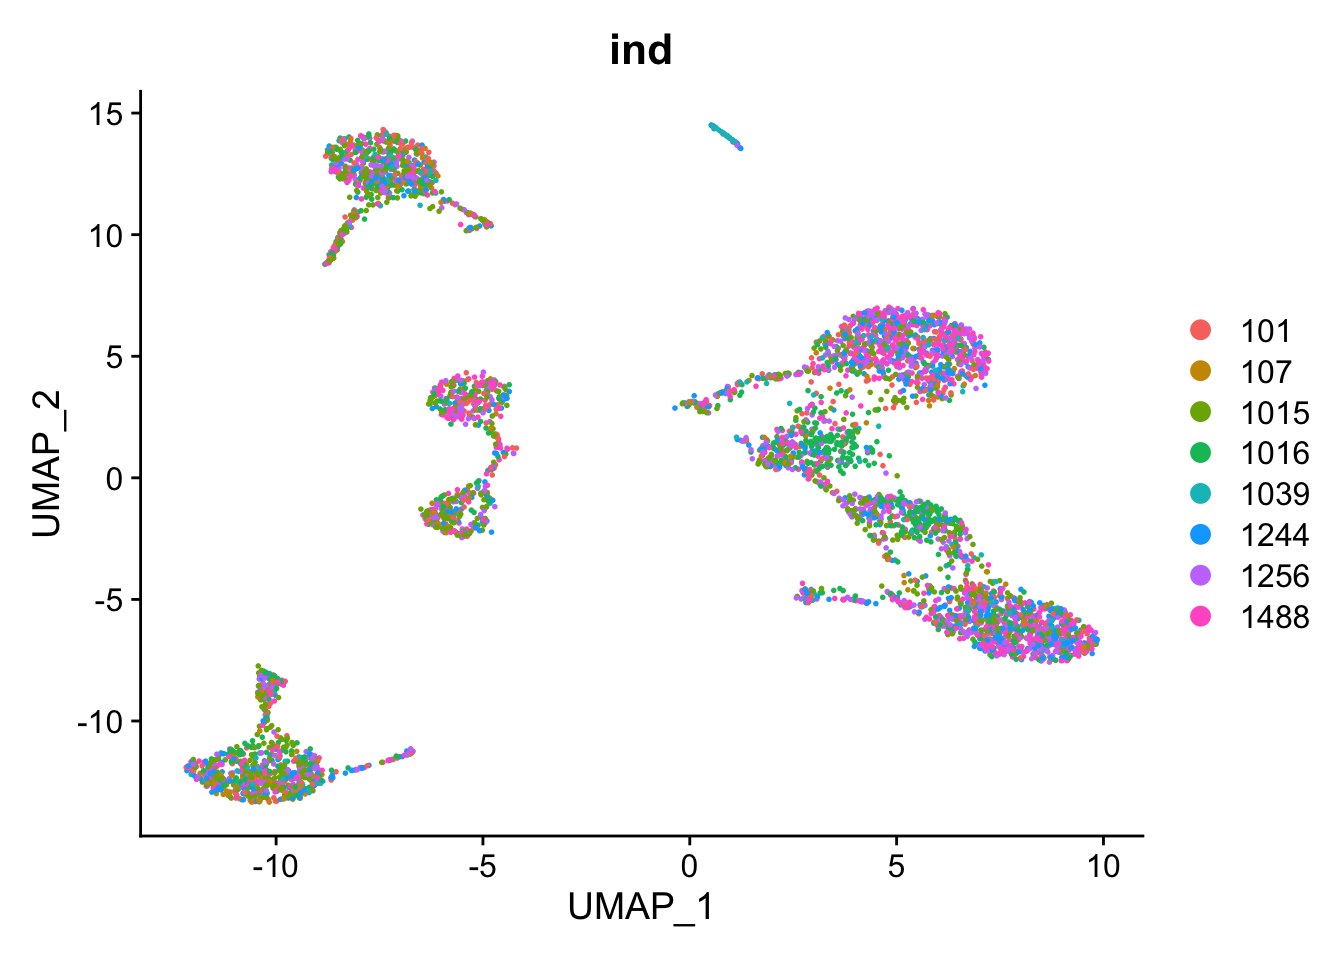
\includegraphics{scRNAseqInR_Doco_files/figure-latex/unnamed-chunk-67-1.pdf}

We can use \texttt{harmony} the same way we used the \texttt{pca} reduction to compute a UMAP layout or to find clusters.

\begin{Shaded}
\begin{Highlighting}[]
\NormalTok{kang }\OtherTok{\textless{}{-}} \FunctionTok{RunUMAP}\NormalTok{(kang, }\AttributeTok{reduction=}\StringTok{"harmony"}\NormalTok{, }\AttributeTok{dims=}\DecValTok{1}\SpecialCharTok{:}\DecValTok{10}\NormalTok{, }\AttributeTok{reduction.name=}\StringTok{"umap\_harmony"}\NormalTok{)}
\CommentTok{\#\textgreater{} 10:37:12 UMAP embedding parameters a = 0.9922 b = 1.112}
\CommentTok{\#\textgreater{} 10:37:12 Read 5000 rows and found 10 numeric columns}
\CommentTok{\#\textgreater{} 10:37:12 Using Annoy for neighbor search, n\_neighbors = 30}
\CommentTok{\#\textgreater{} 10:37:12 Building Annoy index with metric = cosine, n\_trees = 50}
\CommentTok{\#\textgreater{} 0\%   10   20   30   40   50   60   70   80   90   100\%}
\CommentTok{\#\textgreater{} [{-}{-}{-}{-}|{-}{-}{-}{-}|{-}{-}{-}{-}|{-}{-}{-}{-}|{-}{-}{-}{-}|{-}{-}{-}{-}|{-}{-}{-}{-}|{-}{-}{-}{-}|{-}{-}{-}{-}|{-}{-}{-}{-}|}
\CommentTok{\#\textgreater{} **************************************************|}
\CommentTok{\#\textgreater{} 10:37:12 Writing NN index file to temp file /var/folders/tp/b078yqdd4ydff9fx87lfttpj\_sc0x3/T//RtmpVlgEIH/file5f4f2df3373e}
\CommentTok{\#\textgreater{} 10:37:13 Searching Annoy index using 1 thread, search\_k = 3000}
\CommentTok{\#\textgreater{} 10:37:14 Annoy recall = 100\%}
\CommentTok{\#\textgreater{} 10:37:14 Commencing smooth kNN distance calibration using 1 thread with target n\_neighbors = 30}
\CommentTok{\#\textgreater{} 10:37:15 Initializing from normalized Laplacian + noise (using irlba)}
\CommentTok{\#\textgreater{} 10:37:15 Commencing optimization for 500 epochs, with 210490 positive edges}
\CommentTok{\#\textgreater{} 10:37:20 Optimization finished}
\CommentTok{\#\textgreater{} Warning: Cannot add objects with duplicate keys (offending}
\CommentTok{\#\textgreater{} key: UMAP\_), setting key to \textquotesingle{}umap\_harmony\_\textquotesingle{}}

\FunctionTok{DimPlot}\NormalTok{(kang, }\AttributeTok{reduction=}\StringTok{"umap\_harmony"}\NormalTok{, }\AttributeTok{group.by=}\StringTok{"stim"}\NormalTok{)}
\end{Highlighting}
\end{Shaded}

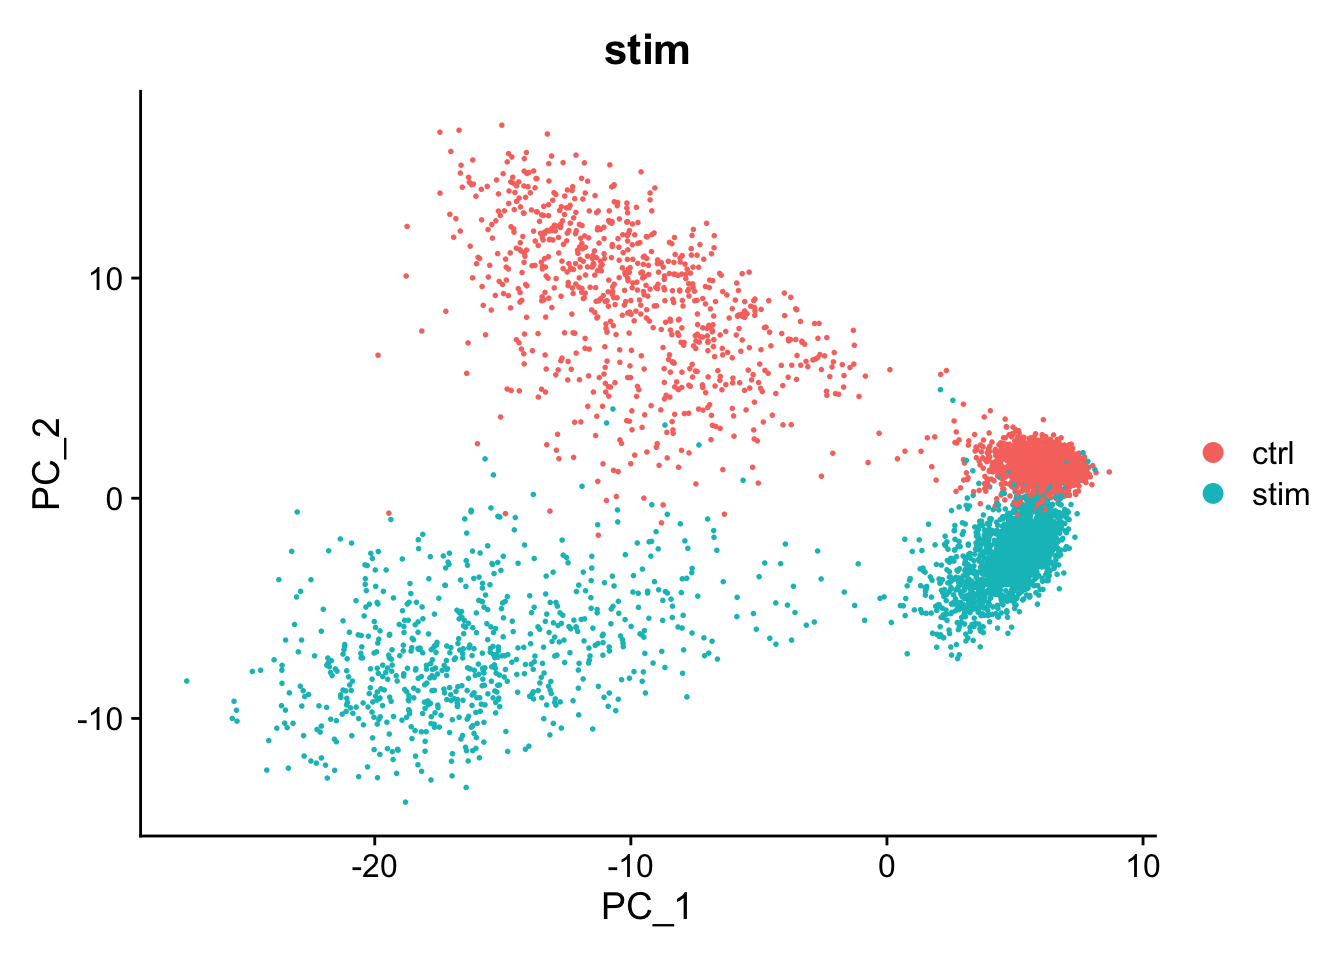
\includegraphics{scRNAseqInR_Doco_files/figure-latex/unnamed-chunk-68-1.pdf}

\begin{Shaded}
\begin{Highlighting}[]

\NormalTok{kang }\OtherTok{\textless{}{-}} \FunctionTok{FindNeighbors}\NormalTok{(kang, }\AttributeTok{reduction=}\StringTok{"harmony"}\NormalTok{, }\AttributeTok{dims=}\DecValTok{1}\SpecialCharTok{:}\DecValTok{10}\NormalTok{)}
\CommentTok{\#\textgreater{} Computing nearest neighbor graph}
\CommentTok{\#\textgreater{} Computing SNN}
\NormalTok{kang }\OtherTok{\textless{}{-}} \FunctionTok{FindClusters}\NormalTok{(kang, }\AttributeTok{resolution=}\FloatTok{0.25}\NormalTok{)}
\CommentTok{\#\textgreater{} Modularity Optimizer version 1.3.0 by Ludo Waltman and Nees Jan van Eck}
\CommentTok{\#\textgreater{} }
\CommentTok{\#\textgreater{} Number of nodes: 5000}
\CommentTok{\#\textgreater{} Number of edges: 171396}
\CommentTok{\#\textgreater{} }
\CommentTok{\#\textgreater{} Running Louvain algorithm...}
\CommentTok{\#\textgreater{} Maximum modularity in 10 random starts: 0.9324}
\CommentTok{\#\textgreater{} Number of communities: 9}
\CommentTok{\#\textgreater{} Elapsed time: 0 seconds}
\NormalTok{kang}\SpecialCharTok{$}\NormalTok{harmony\_clusters }\OtherTok{\textless{}{-}}\NormalTok{ kang}\SpecialCharTok{$}\NormalTok{seurat\_clusters}

\FunctionTok{DimPlot}\NormalTok{(kang, }\AttributeTok{reduction=}\StringTok{"umap\_harmony"}\NormalTok{, }\AttributeTok{group.by=}\StringTok{"harmony\_clusters"}\NormalTok{)}
\end{Highlighting}
\end{Shaded}

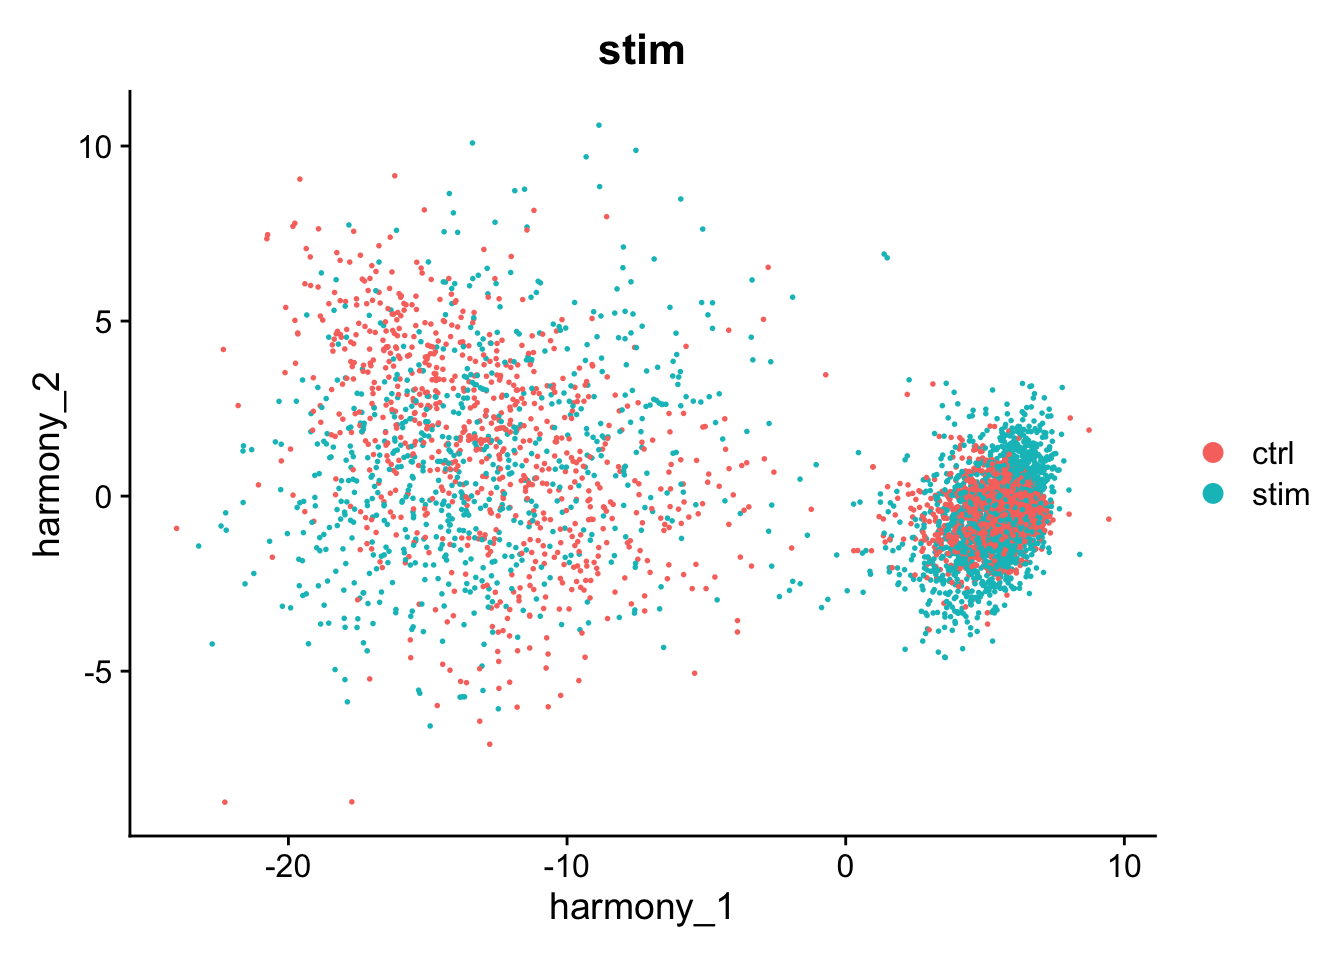
\includegraphics{scRNAseqInR_Doco_files/figure-latex/unnamed-chunk-68-2.pdf}

\begin{Shaded}
\begin{Highlighting}[]
\FunctionTok{DimPlot}\NormalTok{(kang, }\AttributeTok{reduction=}\StringTok{"umap"}\NormalTok{, }\AttributeTok{group.by=}\StringTok{"harmony\_clusters"}\NormalTok{)}
\end{Highlighting}
\end{Shaded}

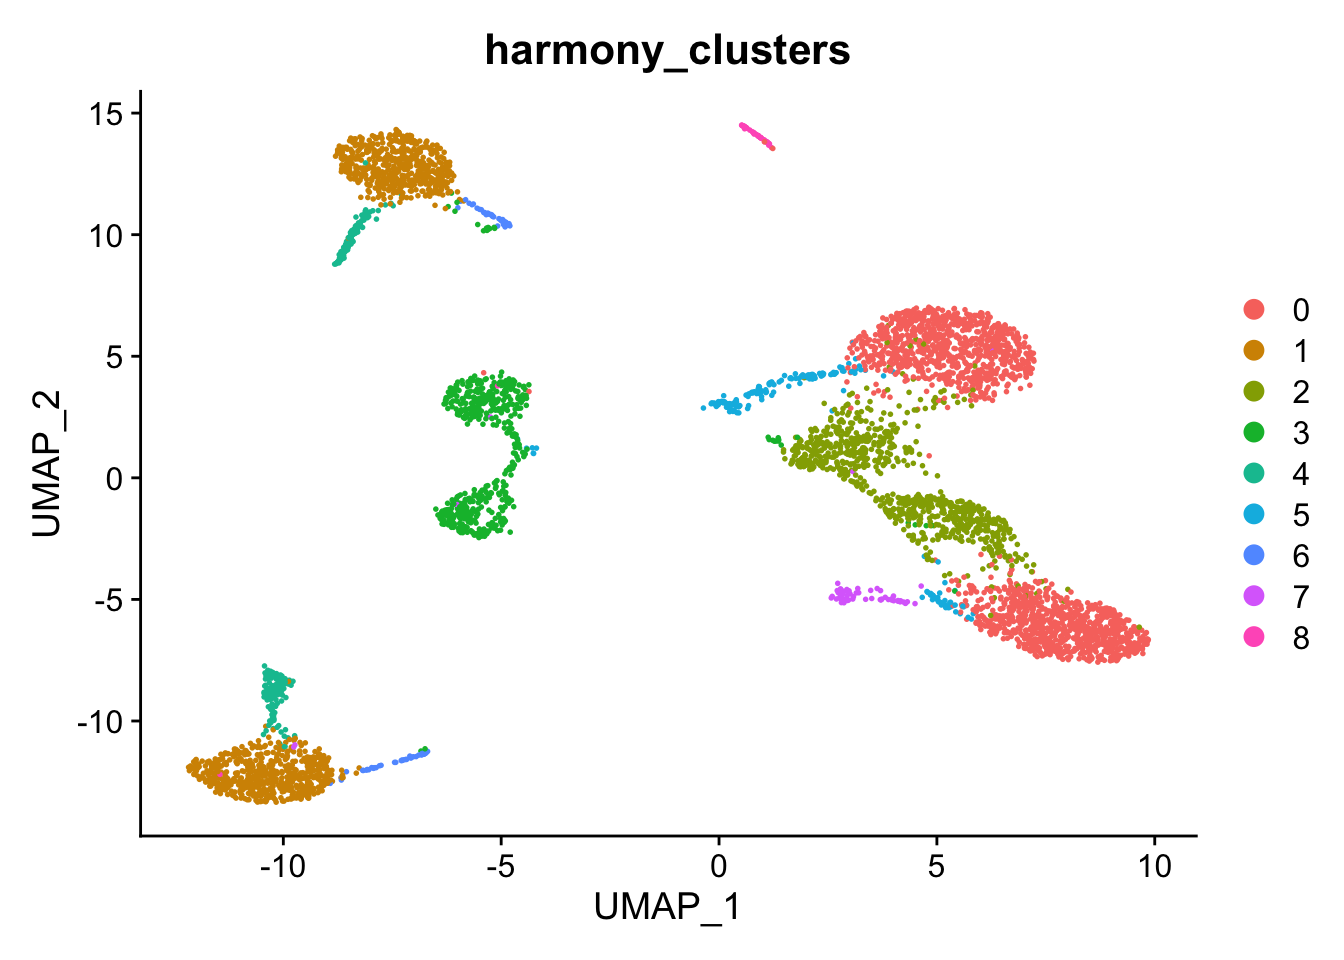
\includegraphics{scRNAseqInR_Doco_files/figure-latex/unnamed-chunk-68-3.pdf}

Having found a good set of clusters, we would usually perform differential expression analysis on the original data and include batches/runs/individuals as predictors in the linear model. In this example we could now compare un-stimulated and stimulated cells within each cluster. A particularly nice statistical approach that is possible here would be to convert the counts to pseudo-bulk data for the eight individuals, and then apply a bulk RNA-Seq differential expression analysis method. However there is still the problem that unstimulated and stimulated cells were processed in separate batches.

\hypertarget{resources}{%
\chapter{Resources}\label{resources}}

Useful resources for next steps.

\hypertarget{help-and-fruther-resources}{%
\section{Help and fruther Resources}\label{help-and-fruther-resources}}

\hypertarget{seurat-vignettes}{%
\subsection*{Seurat Vignettes}\label{seurat-vignettes}}
\addcontentsline{toc}{subsection}{Seurat Vignettes}

\url{https://satijalab.org/seurat/index.html}

There are a good many Seurat vigettes for different aspects of the Seurat package. E.g.

\begin{itemize}
\tightlist
\item
  \href{https://satijalab.org/seurat/articles/pbmc3k_tutorial.html}{Guided Clustering tutorial} : We've just worked through this
\item
  \href{https://satijalab.org/seurat/archive/v3.1/de_vignette.html}{Differential expression} : An Exploration of differential expression methods within Seurat
\item
  \href{https://satijalab.org/seurat/articles/integration_introduction.html}{Data integration} : Seurat's data integration is a popular method to combine different datasets into one joint analysis.
\end{itemize}

\hypertarget{seurat-cheatsheet}{%
\subsection*{Seurat Cheatsheet}\label{seurat-cheatsheet}}
\addcontentsline{toc}{subsection}{Seurat Cheatsheet}

\url{https://satijalab.org/seurat/articles/essential_commands.html}

A useful resource for asking; How can I do `X' with my seurat object?

\hypertarget{osca}{%
\subsection*{OSCA}\label{osca}}
\addcontentsline{toc}{subsection}{OSCA}

\url{https://bioconductor.org/books/release/OSCA/}

An comprehensive resource for analysis approaches for single cell data.
This uses the SingleCellExperiment bioconductor ecosystem, but alot of the same principle still apply.

This includes a good discussion of useing \href{http://bioconductor.org/books/3.15/OSCA.multisample/multi-sample-comparisons.html\#creating-pseudo-bulk-samples}{pseudobulk approaches}, worth checking out for differential expression analyses.

\hypertarget{mbp-training-reading-list}{%
\subsection*{MBP training Reading list}\label{mbp-training-reading-list}}
\addcontentsline{toc}{subsection}{MBP training Reading list}

\url{https://monashbioinformaticsplatform.github.io/Single-Cell-Workshop/}

A workshop page for a previous workshop (upon which this one is based) run by Monash Bioinformatics Platform - down the bottom there
is an extensive list of useful single cell links and resources.

\hypertarget{biocommons-single-cell-omics}{%
\subsection*{Biocommons Single Cell Omics}\label{biocommons-single-cell-omics}}
\addcontentsline{toc}{subsection}{Biocommons Single Cell Omics}

\url{https://www.biocommons.org.au/single-cell-omics}

Join the single cell omics community resources being setup by biocommons.

\begin{center}\rule{0.5\linewidth}{0.5pt}\end{center}

\hypertarget{data}{%
\section{Data}\label{data}}

\hypertarget{demo-10x-data}{%
\subsection*{Demo 10X data}\label{demo-10x-data}}
\addcontentsline{toc}{subsection}{Demo 10X data}

\url{https://www.10xgenomics.com/resources/datasets}

10X genomics have quite a few example datasets availble for download (including PBMC3k).
This is a useful resource if you want to see what the `raw' data looks like for a particular technology.

\hypertarget{geo}{%
\subsection*{GEO}\label{geo}}
\addcontentsline{toc}{subsection}{GEO}

\url{https://www.ncbi.nlm.nih.gov/geo/}

Many papers publish their raw single cell data in GEO. Formats vary, but often you can find the counts matrix.

\hypertarget{seurat-data}{%
\subsection*{Seurat data}\label{seurat-data}}
\addcontentsline{toc}{subsection}{Seurat data}

\url{https://github.com/satijalab/seurat-data}

Package for obtaining a few datasets as seurat objects.

\begin{center}\rule{0.5\linewidth}{0.5pt}\end{center}

\hypertarget{analysis-tools}{%
\section{Analysis Tools}\label{analysis-tools}}

A handful of the many tools that might be worth checking out for next steps.

\hypertarget{cyclone}{%
\subsection*{Cyclone}\label{cyclone}}
\addcontentsline{toc}{subsection}{Cyclone}

\url{https://pubmed.ncbi.nlm.nih.gov/26142758/}

Part of the scran package, cyclone is a(nother) method for determining cell phase.
\href{https://rdrr.io/bioc/scran/man/cyclone.html}{Doco}

\hypertarget{harmony}{%
\subsection*{Harmony}\label{harmony}}
\addcontentsline{toc}{subsection}{Harmony}

\url{https://portals.broadinstitute.org/harmony/articles/quickstart.html}

Method for integration of multiple single cell datasets.

\hypertarget{singler-1}{%
\subsection*{SingleR}\label{singler-1}}
\addcontentsline{toc}{subsection}{SingleR}

\url{http://bioconductor.org/books/release/SingleRBook/}

There is extensive documentation for the singleR package in the `singleR' book.

\hypertarget{scrublet}{%
\subsection*{Scrublet}\label{scrublet}}
\addcontentsline{toc}{subsection}{Scrublet}

\url{https://github.com/swolock/scrublet}

A python based tool for doublet detection. One of many tools in this space.

\hypertarget{scvelo}{%
\subsection*{ScVelo}\label{scvelo}}
\addcontentsline{toc}{subsection}{ScVelo}

\url{https://scvelo.readthedocs.io/}

A package for single cell RNA velocity analysis, useful for developmental/pseudotime trajectories. Python/scanpy based.

\hypertarget{monocle}{%
\subsection*{Monocle}\label{monocle}}
\addcontentsline{toc}{subsection}{Monocle}

\url{https://cole-trapnell-lab.github.io/monocle3/}

A package for single cell developmental//pseudotime trajectory analysis.

\hypertarget{tidyseurat}{%
\subsection*{TidySeurat}\label{tidyseurat}}
\addcontentsline{toc}{subsection}{TidySeurat}

\url{https://stemangiola.github.io/tidyseurat/}

For fans of tidyverse-everything, there's tidyseurat. Example workflow \href{https://tidytranscriptomics-workshops.github.io/bioc2022_tidytranscriptomics/articles/tidytranscriptomics_case_study.html}{here}

\begin{center}\rule{0.5\linewidth}{0.5pt}\end{center}

\hypertarget{preprocessing-tools}{%
\section{Preprocessing Tools}\label{preprocessing-tools}}

Tooks that process raw sequencing data into counts matricies

\hypertarget{cell-ranger}{%
\subsection*{Cell Ranger}\label{cell-ranger}}
\addcontentsline{toc}{subsection}{Cell Ranger}

\url{https://support.10xgenomics.com/single-cell-gene-expression/software/pipelines/latest/what-is-cell-ranger}

CellRanger is the 10X tool that takes raw fastq sequence files and produces the counts matricies that are the starting point for today's analysis. It only works for 10X data.

\hypertarget{starsolo}{%
\subsection*{STARSolo}\label{starsolo}}
\addcontentsline{toc}{subsection}{STARSolo}

STAR is an aligner (which is actually used within cell ranger). STARSolo is a tool for producing counts matricies, and is configurable enough for use with multiple technologies.

\url{https://github.com/alexdobin/STAR/blob/master/docs/STARsolo.md}

  \bibliography{book.bib,packages.bib}

\end{document}
